%%-----------------------------------------------------------------
% header.tex
% General header content for LaTeX paper: notes.tex
% Author: William DeMeo
% Modified: 00.11.04
% Usage: Start document with the lines
%           %%-----------------------------------------------------------------
% header.tex
% General header content for LaTeX paper: notes.tex
% Author: William DeMeo
% Modified: 00.11.04
% Usage: Start document with the lines
%           %%-----------------------------------------------------------------
% header.tex
% General header content for LaTeX paper: notes.tex
% Author: William DeMeo
% Modified: 00.11.04
% Usage: Start document with the lines
%           \input{header}
%           \begin{document}
%        Then add title with commands \title, \author, \maketitle,
%        \tableofcontents, etc.
%%-----------------------------------------------------------------
%**start of header
%\documentclass[notitlepage,12pt]{article}
\documentclass[11pt]{article}
%\documentclass{amsart}
%\usepackage{spconf,amsmath,epsfig}
\usepackage{amsmath,amssymb,amscd,epsfig}

\usepackage{fullpage}

\usepackage{ifthen}

%% Should figures be compiled?
\newboolean{nofigures} % initially false ==> compile with figures
% comment out the following line to compile with figures
%\setboolean{nofigures}{true} 

%% Should citation footnotes on section headings be compiled?
\newboolean{nofootnotes}
% comment out the following line to include all citation foonotes.
\setboolean{nofootnotes}{true} 

%\usepackage{boxedminipage}
\usepackage{theorem}
{\theorembodyfont{\rmfamily} 
 \newtheorem{definition}{Definition}[section]
 \newtheorem{lemma}{Lemma}[section] % Lemmas are for proving theorems and facts
 \newtheorem{prop}{Proposition}[section] % Props state any new results of this document
 \newtheorem{fact}{Fact}[section]   % Facts are for less important, well-known results
 \newtheorem{example}{Example}[section]   
 \newtheorem{theorem}{Theorem}[section]  % Theorems are for important, well-known results
 {\theoremstyle{marginbreak}  
   \newtheorem{define}{}  % This definition style is for the glossary
    \newtheorem{Theorem}{Theorem}[subsection]  % Theorems are for important, well-known results
 }
}
\renewcommand{\thedefine}{}

% THE FILE
%   /usr/share/texmf/doc/latex/hyperref/manual.pdf
%  documents the hyperref package
%\usepackage{hyperref}

% THE FILE
%   /usr/share/texmf/doc/latex/general/lshort.dvi (p.12)
%  documents the pagestyle command
%\pagestyle{headings}
% 2004.03.30: commented next six lines:
%\usepackage{fancyhdr}
%\pagestyle{fancy}
%\lhead{\thesection} \chead{} \rhead{\thepage} 
%\lfoot{Do Not Duplicate} \cfoot{\bfseries CONFIDENTIAL} \rfoot{Do Not Duplicate} 
%\renewcommand{\headrulewidth}{0pt} \renewcommand{\footrulewidth}{0.4pt}

% THE FILE
%   /usr/share/texmf/doc/pdflatex/base/example.tex
% suggests the following:
%\input pdfcolor.tex
%\pdfoutput=1\relax      % turn on PDF output; otherwise output DVI file
                         % this primitive cannot be specified  *after* shipping
                         % out the *first* page
%\pdfpagewidth=8.26in    % page width of PDF output
%\pdfpageheight=11.69in  % page height of PDF output
%\usepackage[pdftex]{graphicx}
%\DeclareGraphicsExtensions{.jpg,.pdf,.mps,.png}

%-------------------------------------------------------------
% Definitions.
% ------------
%\def\HOME{/home/moonchild/pub/research/dsp/DeMeo/Notes}
\def\HOME{/home/sonic/pub/research/dsp/DeMeo/Notes}
\def\R{\mathbb{R}}    % real numbers 
\def\C{\mathbb{C}}    % complex numbers 
\def\e{\mathrm{e}}    % exponential
% Two notations for real part of a complex number
   \def\Real{\mbox{Re}}  %\def\Real{\Re}
% Two notations for integration over R
   \def\integral{\int_{-\infty}^{\infty}}
     %\def\integral{\int_{-\infty}^{+\infty}} 
% Operator Theory
   \def\A{\operatorname{A}}
   \def\E{\operatorname{E}}
   \def\H{\operatorname{H}}
   \def\I{\operatorname{I}}
   \def\P{\operatorname{P}}
   \def\pv{\operatorname{pv}}
   \def\S{\operatorname{S}}
   \def\T{\operatorname{T}}
   \def\W{\operatorname{W}}
   \def\Hilbert{\mathcal{H}}
   \def\Hone{\mathcal{H}_1}
   \def\Htwo{\mathcal{H}_2}
   \def\Banach{\mathcal{B}(\Hilbert,\Hilbert)}
   \def\Banachonetwo{\mathcal{B}(\Hone,\Htwo)}
   \def\Banachtwoone{\mathcal{B}(\Htwo,\Hone)}
   \def\Lone{L^1}
   \def\Ltwo{L^2}
   \def\ltwo{\ell^2}
   \def\LoneR{L^1(\mathbb{R})}
   \def\LtwoR{L^2(\mathbb{R})}
   \def\ltwoR{\ell^2(\mathbb{R})}
   \def\Null{\mathcal{N}}  % nullspace
% Signals, Time-Frequency shifts, etc.
   \def\scale{\frac{1}{\sqrt{s}}}
   \def\transcale{\left(\frac{t-u}{s}\right)}
   \def\xpull{x_{\frac{\tau}{2}, -\frac{\xi}{2}}}
   \def\xpush{x_{-\frac{\tau}{2}, \frac{\xi}{2}}}
   \def\xpullpush{x_{\frac{\tau}{2}, \frac{\xi}{2}}}
   \def\xpushpull{x_{-\frac{\tau}{2}, -\frac{\xi}{2}}}
   \def\xfpull{x_{-\frac{\Delta\nu}{2}}}
   \def\xfpush{x_{\frac{\Delta\nu}{2}}}
   \def\apull{a_{-}}
   \def\apush{a_{+}}

   \def\ytnu{y_{t,\nu}}
   \def\ytnut{\tilde{y}_{t,\nu}}
   \def\half{{\scriptstyle \frac{1}{2}}}
   \def\halftau{{\scriptstyle \frac{\tau}{2}}}
   \def\halfxi{{\scriptstyle \frac{\xi}{2}}}
   \def\halfnu{{\scriptstyle \frac{\nu}{2}}}
   \def\halfDnu{{\scriptstyle \frac{\Delta\nu}{2}}}

   \def\xtpull{x\left(t+\halftau\right)}
   \def\xtpush{x\left(t-\halftau\right)}
%   (shouldn't need this) \def\xtpullconj{x^*\left(t+\halftau\right)}
   \def\xtpushconj{x^*\left(t-\halftau\right)}
   \def\Xtpull{X\left(\nu+\halfxi\right)}
   \def\Xtpush{X\left(\nu-\halfxi\right)}
   \def\Xtpullconj{X^*\left(\nu+\halfxi\right)}
%   (shouldn't need this) \def\Xtpushconj{X^*\left(\nu-\halfxi\right)}

   \def\ytpull{y\left(t+\halftau\right)}
   \def\ytpush{y\left(t-\halftau\right)}
%   (shouldn't need this) \def\ytpullconj{y^*\left(t+\halftau\right)}
   \def\ytpushconj{y^*\left(t-\halftau\right)}
   \def\Ytpull{Y\left(\nu+\halfxi\right)}
   \def\Ytpush{Y\left(\nu-\halfxi\right)}
   \def\Ytpullconj{Y^*\left(\nu+\halfxi\right)}
%   (shouldn't need this) \def\Ytpushconj{Y^*\left(\nu-\halfxi\right)}

% Language
   \def\FT{Fourier transform}
   \def\WT{Wigner transform}
   \def\WV{Wigner-Ville}

%%-------------------------------------------------------------
%**end of header
%\includeonly{./theory/ambiguity,./theory/energydensity}

%           \begin{document}
%        Then add title with commands \title, \author, \maketitle,
%        \tableofcontents, etc.
%%-----------------------------------------------------------------
%**start of header
%\documentclass[notitlepage,12pt]{article}
\documentclass[11pt]{article}
%\documentclass{amsart}
%\usepackage{spconf,amsmath,epsfig}
\usepackage{amsmath,amssymb,amscd,epsfig}

\usepackage{fullpage}

\usepackage{ifthen}

%% Should figures be compiled?
\newboolean{nofigures} % initially false ==> compile with figures
% comment out the following line to compile with figures
%\setboolean{nofigures}{true} 

%% Should citation footnotes on section headings be compiled?
\newboolean{nofootnotes}
% comment out the following line to include all citation foonotes.
\setboolean{nofootnotes}{true} 

%\usepackage{boxedminipage}
\usepackage{theorem}
{\theorembodyfont{\rmfamily} 
 \newtheorem{definition}{Definition}[section]
 \newtheorem{lemma}{Lemma}[section] % Lemmas are for proving theorems and facts
 \newtheorem{prop}{Proposition}[section] % Props state any new results of this document
 \newtheorem{fact}{Fact}[section]   % Facts are for less important, well-known results
 \newtheorem{example}{Example}[section]   
 \newtheorem{theorem}{Theorem}[section]  % Theorems are for important, well-known results
 {\theoremstyle{marginbreak}  
   \newtheorem{define}{}  % This definition style is for the glossary
    \newtheorem{Theorem}{Theorem}[subsection]  % Theorems are for important, well-known results
 }
}
\renewcommand{\thedefine}{}

% THE FILE
%   /usr/share/texmf/doc/latex/hyperref/manual.pdf
%  documents the hyperref package
%\usepackage{hyperref}

% THE FILE
%   /usr/share/texmf/doc/latex/general/lshort.dvi (p.12)
%  documents the pagestyle command
%\pagestyle{headings}
% 2004.03.30: commented next six lines:
%\usepackage{fancyhdr}
%\pagestyle{fancy}
%\lhead{\thesection} \chead{} \rhead{\thepage} 
%\lfoot{Do Not Duplicate} \cfoot{\bfseries CONFIDENTIAL} \rfoot{Do Not Duplicate} 
%\renewcommand{\headrulewidth}{0pt} \renewcommand{\footrulewidth}{0.4pt}

% THE FILE
%   /usr/share/texmf/doc/pdflatex/base/example.tex
% suggests the following:
%\input pdfcolor.tex
%\pdfoutput=1\relax      % turn on PDF output; otherwise output DVI file
                         % this primitive cannot be specified  *after* shipping
                         % out the *first* page
%\pdfpagewidth=8.26in    % page width of PDF output
%\pdfpageheight=11.69in  % page height of PDF output
%\usepackage[pdftex]{graphicx}
%\DeclareGraphicsExtensions{.jpg,.pdf,.mps,.png}

%-------------------------------------------------------------
% Definitions.
% ------------
%\def\HOME{/home/moonchild/pub/research/dsp/DeMeo/Notes}
\def\HOME{/home/sonic/pub/research/dsp/DeMeo/Notes}
\def\R{\mathbb{R}}    % real numbers 
\def\C{\mathbb{C}}    % complex numbers 
\def\e{\mathrm{e}}    % exponential
% Two notations for real part of a complex number
   \def\Real{\mbox{Re}}  %\def\Real{\Re}
% Two notations for integration over R
   \def\integral{\int_{-\infty}^{\infty}}
     %\def\integral{\int_{-\infty}^{+\infty}} 
% Operator Theory
   \def\A{\operatorname{A}}
   \def\E{\operatorname{E}}
   \def\H{\operatorname{H}}
   \def\I{\operatorname{I}}
   \def\P{\operatorname{P}}
   \def\pv{\operatorname{pv}}
   \def\S{\operatorname{S}}
   \def\T{\operatorname{T}}
   \def\W{\operatorname{W}}
   \def\Hilbert{\mathcal{H}}
   \def\Hone{\mathcal{H}_1}
   \def\Htwo{\mathcal{H}_2}
   \def\Banach{\mathcal{B}(\Hilbert,\Hilbert)}
   \def\Banachonetwo{\mathcal{B}(\Hone,\Htwo)}
   \def\Banachtwoone{\mathcal{B}(\Htwo,\Hone)}
   \def\Lone{L^1}
   \def\Ltwo{L^2}
   \def\ltwo{\ell^2}
   \def\LoneR{L^1(\mathbb{R})}
   \def\LtwoR{L^2(\mathbb{R})}
   \def\ltwoR{\ell^2(\mathbb{R})}
   \def\Null{\mathcal{N}}  % nullspace
% Signals, Time-Frequency shifts, etc.
   \def\scale{\frac{1}{\sqrt{s}}}
   \def\transcale{\left(\frac{t-u}{s}\right)}
   \def\xpull{x_{\frac{\tau}{2}, -\frac{\xi}{2}}}
   \def\xpush{x_{-\frac{\tau}{2}, \frac{\xi}{2}}}
   \def\xpullpush{x_{\frac{\tau}{2}, \frac{\xi}{2}}}
   \def\xpushpull{x_{-\frac{\tau}{2}, -\frac{\xi}{2}}}
   \def\xfpull{x_{-\frac{\Delta\nu}{2}}}
   \def\xfpush{x_{\frac{\Delta\nu}{2}}}
   \def\apull{a_{-}}
   \def\apush{a_{+}}

   \def\ytnu{y_{t,\nu}}
   \def\ytnut{\tilde{y}_{t,\nu}}
   \def\half{{\scriptstyle \frac{1}{2}}}
   \def\halftau{{\scriptstyle \frac{\tau}{2}}}
   \def\halfxi{{\scriptstyle \frac{\xi}{2}}}
   \def\halfnu{{\scriptstyle \frac{\nu}{2}}}
   \def\halfDnu{{\scriptstyle \frac{\Delta\nu}{2}}}

   \def\xtpull{x\left(t+\halftau\right)}
   \def\xtpush{x\left(t-\halftau\right)}
%   (shouldn't need this) \def\xtpullconj{x^*\left(t+\halftau\right)}
   \def\xtpushconj{x^*\left(t-\halftau\right)}
   \def\Xtpull{X\left(\nu+\halfxi\right)}
   \def\Xtpush{X\left(\nu-\halfxi\right)}
   \def\Xtpullconj{X^*\left(\nu+\halfxi\right)}
%   (shouldn't need this) \def\Xtpushconj{X^*\left(\nu-\halfxi\right)}

   \def\ytpull{y\left(t+\halftau\right)}
   \def\ytpush{y\left(t-\halftau\right)}
%   (shouldn't need this) \def\ytpullconj{y^*\left(t+\halftau\right)}
   \def\ytpushconj{y^*\left(t-\halftau\right)}
   \def\Ytpull{Y\left(\nu+\halfxi\right)}
   \def\Ytpush{Y\left(\nu-\halfxi\right)}
   \def\Ytpullconj{Y^*\left(\nu+\halfxi\right)}
%   (shouldn't need this) \def\Ytpushconj{Y^*\left(\nu-\halfxi\right)}

% Language
   \def\FT{Fourier transform}
   \def\WT{Wigner transform}
   \def\WV{Wigner-Ville}

%%-------------------------------------------------------------
%**end of header
%\includeonly{./theory/ambiguity,./theory/energydensity}

%           \begin{document}
%        Then add title with commands \title, \author, \maketitle,
%        \tableofcontents, etc.
%%-----------------------------------------------------------------
%**start of header
%\documentclass[notitlepage,12pt]{article}
\documentclass[11pt]{article}
%\documentclass{amsart}
%\usepackage{spconf,amsmath,epsfig}
\usepackage{amsmath,amssymb,amscd,epsfig}

\usepackage{fullpage}

\usepackage{ifthen}

%% Should figures be compiled?
\newboolean{nofigures} % initially false ==> compile with figures
% comment out the following line to compile with figures
%\setboolean{nofigures}{true} 

%% Should citation footnotes on section headings be compiled?
\newboolean{nofootnotes}
% comment out the following line to include all citation foonotes.
\setboolean{nofootnotes}{true} 

%\usepackage{boxedminipage}
\usepackage{theorem}
{\theorembodyfont{\rmfamily} 
 \newtheorem{definition}{Definition}[section]
 \newtheorem{lemma}{Lemma}[section] % Lemmas are for proving theorems and facts
 \newtheorem{prop}{Proposition}[section] % Props state any new results of this document
 \newtheorem{fact}{Fact}[section]   % Facts are for less important, well-known results
 \newtheorem{example}{Example}[section]   
 \newtheorem{theorem}{Theorem}[section]  % Theorems are for important, well-known results
 {\theoremstyle{marginbreak}  
   \newtheorem{define}{}  % This definition style is for the glossary
    \newtheorem{Theorem}{Theorem}[subsection]  % Theorems are for important, well-known results
 }
}
\renewcommand{\thedefine}{}

% THE FILE
%   /usr/share/texmf/doc/latex/hyperref/manual.pdf
%  documents the hyperref package
%\usepackage{hyperref}

% THE FILE
%   /usr/share/texmf/doc/latex/general/lshort.dvi (p.12)
%  documents the pagestyle command
%\pagestyle{headings}
% 2004.03.30: commented next six lines:
%\usepackage{fancyhdr}
%\pagestyle{fancy}
%\lhead{\thesection} \chead{} \rhead{\thepage} 
%\lfoot{Do Not Duplicate} \cfoot{\bfseries CONFIDENTIAL} \rfoot{Do Not Duplicate} 
%\renewcommand{\headrulewidth}{0pt} \renewcommand{\footrulewidth}{0.4pt}

% THE FILE
%   /usr/share/texmf/doc/pdflatex/base/example.tex
% suggests the following:
%\input pdfcolor.tex
%\pdfoutput=1\relax      % turn on PDF output; otherwise output DVI file
                         % this primitive cannot be specified  *after* shipping
                         % out the *first* page
%\pdfpagewidth=8.26in    % page width of PDF output
%\pdfpageheight=11.69in  % page height of PDF output
%\usepackage[pdftex]{graphicx}
%\DeclareGraphicsExtensions{.jpg,.pdf,.mps,.png}

%-------------------------------------------------------------
% Definitions.
% ------------
%\def\HOME{/home/moonchild/pub/research/dsp/DeMeo/Notes}
\def\HOME{/home/sonic/pub/research/dsp/DeMeo/Notes}
\def\R{\mathbb{R}}    % real numbers 
\def\C{\mathbb{C}}    % complex numbers 
\def\e{\mathrm{e}}    % exponential
% Two notations for real part of a complex number
   \def\Real{\mbox{Re}}  %\def\Real{\Re}
% Two notations for integration over R
   \def\integral{\int_{-\infty}^{\infty}}
     %\def\integral{\int_{-\infty}^{+\infty}} 
% Operator Theory
   \def\A{\operatorname{A}}
   \def\E{\operatorname{E}}
   \def\H{\operatorname{H}}
   \def\I{\operatorname{I}}
   \def\P{\operatorname{P}}
   \def\pv{\operatorname{pv}}
   \def\S{\operatorname{S}}
   \def\T{\operatorname{T}}
   \def\W{\operatorname{W}}
   \def\Hilbert{\mathcal{H}}
   \def\Hone{\mathcal{H}_1}
   \def\Htwo{\mathcal{H}_2}
   \def\Banach{\mathcal{B}(\Hilbert,\Hilbert)}
   \def\Banachonetwo{\mathcal{B}(\Hone,\Htwo)}
   \def\Banachtwoone{\mathcal{B}(\Htwo,\Hone)}
   \def\Lone{L^1}
   \def\Ltwo{L^2}
   \def\ltwo{\ell^2}
   \def\LoneR{L^1(\mathbb{R})}
   \def\LtwoR{L^2(\mathbb{R})}
   \def\ltwoR{\ell^2(\mathbb{R})}
   \def\Null{\mathcal{N}}  % nullspace
% Signals, Time-Frequency shifts, etc.
   \def\scale{\frac{1}{\sqrt{s}}}
   \def\transcale{\left(\frac{t-u}{s}\right)}
   \def\xpull{x_{\frac{\tau}{2}, -\frac{\xi}{2}}}
   \def\xpush{x_{-\frac{\tau}{2}, \frac{\xi}{2}}}
   \def\xpullpush{x_{\frac{\tau}{2}, \frac{\xi}{2}}}
   \def\xpushpull{x_{-\frac{\tau}{2}, -\frac{\xi}{2}}}
   \def\xfpull{x_{-\frac{\Delta\nu}{2}}}
   \def\xfpush{x_{\frac{\Delta\nu}{2}}}
   \def\apull{a_{-}}
   \def\apush{a_{+}}

   \def\ytnu{y_{t,\nu}}
   \def\ytnut{\tilde{y}_{t,\nu}}
   \def\half{{\scriptstyle \frac{1}{2}}}
   \def\halftau{{\scriptstyle \frac{\tau}{2}}}
   \def\halfxi{{\scriptstyle \frac{\xi}{2}}}
   \def\halfnu{{\scriptstyle \frac{\nu}{2}}}
   \def\halfDnu{{\scriptstyle \frac{\Delta\nu}{2}}}

   \def\xtpull{x\left(t+\halftau\right)}
   \def\xtpush{x\left(t-\halftau\right)}
%   (shouldn't need this) \def\xtpullconj{x^*\left(t+\halftau\right)}
   \def\xtpushconj{x^*\left(t-\halftau\right)}
   \def\Xtpull{X\left(\nu+\halfxi\right)}
   \def\Xtpush{X\left(\nu-\halfxi\right)}
   \def\Xtpullconj{X^*\left(\nu+\halfxi\right)}
%   (shouldn't need this) \def\Xtpushconj{X^*\left(\nu-\halfxi\right)}

   \def\ytpull{y\left(t+\halftau\right)}
   \def\ytpush{y\left(t-\halftau\right)}
%   (shouldn't need this) \def\ytpullconj{y^*\left(t+\halftau\right)}
   \def\ytpushconj{y^*\left(t-\halftau\right)}
   \def\Ytpull{Y\left(\nu+\halfxi\right)}
   \def\Ytpush{Y\left(\nu-\halfxi\right)}
   \def\Ytpullconj{Y^*\left(\nu+\halfxi\right)}
%   (shouldn't need this) \def\Ytpushconj{Y^*\left(\nu-\halfxi\right)}

% Language
   \def\FT{Fourier transform}
   \def\WT{Wigner transform}
   \def\WV{Wigner-Ville}

%%-------------------------------------------------------------
%**end of header
%\includeonly{./theory/ambiguity,./theory/energydensity}

\thispagestyle{empty}
\newcommand{\HRule}{\rule{\linewidth}{1mm}}
\setlength{\parindent}{0mm}
\setlength{\parskip}{0mm}
\begin{document}
%%% BEGIN: title page
\vspace*{\stretch{1}}
\HRule
  \begin{flushleft}
        \Huge SoundMathWorks \\[5mm]
        \Large Technical Report: \large spectral analysis of music
  \end{flushleft}
\HRule
\vspace*{\stretch{2}}
  \begin{center}
%    \begin{tabular}{cc}
     William J. DeMeo%& co-author's name
%    \end{tabular}
  \end{center}

\pagebreak
%% END: title page
\vspace*{10mm}
\HRule
  \begin{flushleft}
     \Huge SoundMathWorks\\[5mm]
     \Large Technical Report: 
     \large spectral analysis of music\hspace*{\stretch{1}} 23 July 2001
  \end{flushleft}
\HRule\\
\begin{center}
%\begin{tabular}{ccc}
William J. DeMeo\\%&& co-author's name \\
{\small {\tt william.demeo@verizon.net}}%&&{\small {\tt co-author's email}}\\
%\end{tabular}
\end{center}
\vspace{10mm}

% 2004.03.30: commented next five lines
%\pagestyle{fancy}
%\lhead{DO NOT DUPLICATE} \chead{\bfseries CONFIDENTIAL} \rhead{DO NOT DUPLICATE} 
%\lfoot{} \cfoot{\thepage} \rfoot{}
%%\renewcommand{\headrulewidth}{0.4pt} \renewcommand{\footrulewidth}{0.4pt} 
%\renewcommand{\headrulewidth}{0.2pt} \renewcommand{\footrulewidth}{0pt}

\tableofcontents
\setlength{\parindent}{5mm}

\begin{abstract}
This paper describes new and existing methods for representing,
analyzing, and modifying the information content of musical signals.
In particular, the primary objective is to find signal representations
well suited for the analysis and understanding of the human perception
of music.  In pursuit of this objective, we consider how to use such
representations to make inferences about a listener's musical preferences
concerning the represented signal.  We also consider ways in which special
signal representations can facilitate signal modifications accroding to
given musical criteria.
\end{abstract}


% -*- mode: LaTeX; tex-main-file: "../notes.tex"; -*-
%\begin{itemize}
%\item Synthesis -- Sethares (p.15), comp book (00.07.17), beige book (00.07.27)
%\item Tonal Fusion -- comp book (00.07.10)
%\item Spectral Dominance -- Hartmann (p.298) and beige book (00.07.11)
%\item Tonal Dissonance -- comp book (00.07.21)
%\item Wavelet Theory -- beige book (00.07.31, 00.08.01, 00.08.02)
%\end{itemize}
%\subsection{Introduction\protect\footnotemark}
\footnotetext{The quote is from Mallat~\cite{Mallat:1998} p.~1.}  
\begin{quote}
``After a few minutes in a restaurant we cease to notice the annoying
hubbub of surrounding conversations, but a sudden silence reminds us
of the presence of neighbors.  Our attention is clearly attracted by
transients and movements as opposed to stationary stimuli, which we
soon ignore.  Concentrating on transients is probably a strategy for
selecting important information from the overwhelming amount of data
recorded by our senses. Yet, classical signal processing has devoted
most of its efforts to the design of time-invariant and
space-invariant operators, that modify stationary signal properties.
This has led to the indisputable hegemony of the Fourier transform,
but leaves aside many information-processing applications.

The world of transients is considerably larger and more complex than
the garden of stationary signals.  The search for an ideal
Fourier-like basis that would simplify most signal processing is
therefore a hopeless quest.  Instead, a multitude of different
transforms and bases have proliferated, among which wavelets are just
one example.''
\end{quote}

                                                                            
\section{Introduction}
\subsection{Analysis of Non-stationary Signals}
There is a vast literature on the analysis of signals -- be they
musical or not.  The broad class of analysis methods that we study here
consists of {\it time-frequency representations}.  The type of signal
which concerns us is a {\it time series}, $x(t)$.  In other words, it
is a function of a single time variable, $t$.  Often there is reason
to believe that periodicities play an important role in the structure
of $x(t)$.  To study the signal from this point of view, we decompose
it as a function of both time and frequency. Such a decomposition is
what we mean by a time-frequency representation (TFR).

The two broad classes of TFR's which we consider are {\it atomic
decompositions} and {\it energy distributions}.  The first decomposes a
signal by ``projecting'' it onto the time-frequency space, thereby equating
it with a weighted sum of basic elements in that space. (These basic elements
do not always comprise a {\it basis} -- a full set of orthonormal 
elements -- and, in such cases, the decomposition is not a true projection.)
A few more comments about atomic decompositions appear below, but a more
detailed discussion appears is section~\ref{sec:atomic}.

The second class of TFR's are the energy distributions, the primary
objective of which is to represent a distribution of the signal's energy
across the time-frequency plane.  We consider the energy distributions in
section~\ref{sec:energy}. 

Before proceeding, let's consider some general, motivating comments
concerning the use of atomic decompositions for our application.  The
primary consideration for such analyses is the selection an appropriate
basis for processing a particular class of signals.  
%\begin{quote}
The decomposition coefficients of a signal in a basis define a representation 
that highlights some particular signal properties.  For example, wavelet
coefficients provide explicit information on the location and type of signal
singularities.  The problem is to find a criterion for selecting a basis that
is intrinsically well adapted to represent a class of signals.
%\end{quote}

Using classical Fourier analysis, a signal $x$ can be decomposed as a
weighted sum of sinusoidal functions, $\{e^{i2\pi \xi t}\}$,
\[
x(t) = %\frac{1}{2\pi}
\integral X(\xi) e^{i2\pi \xi t}\, d\xi
\]
with weights (amplitudes) given by the Fourier transform
%$X(\xi)$, 
of $x$:
\begin{equation}
\label{eqn:ft}
X(\xi) = \int_{-\infty}^{\infty}x(t) e^{-i2\pi \xi t}\, dt
\end{equation}
If our focus is limited to stationary signals whose frequency contents
do not change dramatically with time, the Fourier analysis provides
simple answers to most questions.  However, we are interested in
representing transient phenomena -- e.g.~a sudden change or singularity in a 
musical signal -- and the Fourier transform is the wrong tool for the job.

The Fourier coefficient in~(\ref{eqn:ft}) is obtained by correlating $x$
with a sinusoidal wave $e^{i2\pi\xi t}$.  Since the support 
of $e^{i2\pi\xi t}$ covers the whole real line, $X(\xi)$ depends 
on the values $x(t)$ for all times $t \in \R$.  This global ``mix'' of
information makes it difficult to analyze any local property of $x$
from $X$.  We need to consider using local time-frequency
transforms, such as the windowed Fourier transform and wavelet
transform, which decompose the signal over waveforms that are well
localized in both frequency and time.

Though wavelet and windowed Fourier techniques can be effectively applied to
non-stationary signals, they suffer from the adverse consequences of
Heisenberg's uncertainty principle.  In TFR analyses, the manifestation of
this principle is the time-frequency resolution trade-off which is
described in section~\ref{sec:atom-decomp}.  Addressing this problem are the
more general distributions of section~\ref{sec:energy}. 

\subsection{Signal Processing for Perception Analysis}
A second objective of this work is to derive new methods and software
routines for a \emph{perception analysis} of a piece of music, $x(t)$.
We consider the aforementioned signal analysis methods in light of this objective,
and focus on those methods which
%a piece of music in such a way that 
facilitate measures of perceived qualities of music.  More specifically, we
consider how signal energy densities relate to a quantitative measure of
\emph{sensory dissonance}, which we define in section~\ref{sec:consonance}. 

There are great challenges to overcome even when we limit our scope to the
spectral analysis outlined in the preceding section.  By further
stipulating that this will then serve as a foundation for the analysis of
perceptions of musical signals, we significantly increase the problem's
complexity. Thus, it is helpful to consider what we should take to be the
primary tasks involved in reaching our objective.  The following is a rough
description of these tasks:
\begin{enumerate}
\item \label{item:spectral} Find useful time-frequency representations for
  analyzing the information content of $x(t)$, with the goal of characterizing
  perceptual  properties of the signal.
\item \label{item:dissonance} Exploiting the analyses of~\ref{item:spectral},
  derive measures of qualities related to human perception of the signal.
  Derive the ``consonance signature'' of $x(t)$. 
\item Create methods for altering the consonance signature of $x(t)$, by
  manipulating the structure of its time-frequency representation (e.g.~using
  time-frequency transformations).
\end{enumerate}

Our approach to (\ref{item:spectral}) considers the atomic decompositions
(e.g.~windowed Fourier or wavelet analysis), as well as energy distributions. 
Concerning the former, the ``grains'' of \emph{granular synthesis} (Cavalierre
and Piccialli~\cite{Cavaliere:1997},~\cite{Roads:1997}) usually represent
segments of the signal that extend beyond a single period. The goal is to
capture the pseudo-periodic component of the signal. For wavelet analyses, we
could attempt to find a basis whose elements are closely correlated with the
components of the signal having the greatest ``periodic endurance.''
We decompose the signal into its quasi-harmonic part (wavelet
components) and its \emph{transients} (error terms, deviations,
micro-variants):
\[
x(t) = \P_{\mathcal{M}}[x](t) 
       + [x(t) - \P_{\mathcal{M}}[x](t)]
\]
The first term on the right is the orthogonal projection of $x$
onto the ``harmonic'' subspace $\mathcal{M}$.  The second term
accounts for the part of $x$ that is orthogonal to the harmonic
subspace (i.e.~the transients).

To address item (\ref{item:dissonance}), we might consider various
decompositions of frequency space $F,$ for instance, as a direct sum
of subspaces $\{S_1, S_2, \ldots, S_N\}$: 
\[ F = S_1 \oplus S_2 \oplus \cdots \oplus S_N\]
where each $S_k$ defines a \emph{subspace of great consonance.}
This could be taken to mean that tones occurring within 
the same subspace, say $x \in S_k$ and  $x' \in S_k,$ are relatively
consonant, while $x$ and  
$y \in S_{k+1}$ are relatively dissonant.  We could also specify some
properties that such subspaces should posses. For example, let $S_k$
and $S_{k+1}$ be two distinct subspaces of great consonance and
suppose $x \in S_k$ and $y \in S_{k+1}$.  Then, 
\[
D(x,x') \leq D(x,y) \mbox{ for any } x' \in S_k
\] 
More precisely, this is a property of the \emph{dissonance metric}
$D(\cdot,\cdot)$ defined on the space, which leads us to the issue of how
dissonance ought to be defined.

% (begin: input from icassp paper, file Intro.tex}

The concept of \emph{sensory dissonance} was originally proposed
by Helmholtz \cite{Helmholtz:1877}, and further developed by Plomp and 
Levelt~\cite{Plomp:1965}, and Sethares~\cite{Sethares:1997}.
Though we consider these studies in greater detail in
sections~\ref{sec:consonance} and~\ref{sec:disscurves}, what follows
is a descriptions that motivates our alternative treatment of this
subject. 

In order to assess the intrinsic dissonance of a musical signal over a
small time interval, the aforementioned studies employ a function of
the the signal's estimated frequency components over that interval.
This often provides a useful quantitative measure.  However, such a
function makes no attempt to account for other widely accepted notions
of dissonance.   
Perhaps the most obvious short-coming results from the point-wise
nature of the dissonance function.  That is, because it is
well localized in time, the dissonance function does not 
measure the \emph{melodic dissonance} of the signal.  The melodic
dissonance of a given segment of music depends on that 
segment's relation to its context.  In our present work, we
consider signal analysis methods that provide for
%estimates of
%instantaneous frequencies and analytic amplitudes of a signal, and use 
%these estimates to measure the dissonance properties of the
%signal.  A primary objective is the development of methods providing
more dynamic dissonance measures, simultaneously accounting for local
dissonance as well as melodic contour.

% (end: input from icassp paper, file Intro.tex}

% -*- mode: LaTeX; tex-main-file: "../Notes.tex"; -*-
\section{Background: Musical Signals}
\subsection{Mathematics of the Pure Tone}
The pure tone is the most elementary of all signals
(Hartmann~\cite{Hartmann:1998}).  Mathematically it is known as the
sine wave, a function of time described by the equation 
\begin{equation}
\label{eqn:puretone}
x(t) = A \sin(2 \pi t/T + \phi)
\end{equation}
where $A$ is the \emph{amplitude}, $T$ is the \emph{period} in
seconds, and $\phi$ is the \emph{phase} in radians.  The units of $x$,
whatever they might be (mechanical displacement, pressure, voltage),
are the same as the units of the amplitude $A$.

The sine function is periodic; it repeats itself when its argument,
the \emph{instantaneous phase} $2\pi t/T + \phi$, changes by $2\pi$.
Equation~(\ref{eqn:puretone}) shows that if $t$ starts at $t_0$ and
increases to $t_0 + T$, the function comes back to its starting
point; that is,
\[x(t_0) = x(t_0 + T)\]
This is why $T$ is called the period, measured in units of seconds per
cycle.  Its inverse, measured in units of cycles per second (Hz) is
called the \emph{frequency} of the wave,
\[f = 1/T\]
Because there are $2 \pi$ radians in a cycle, the \emph{angular
frequency}, $\omega$, is related to the frequency by 
\[\omega = 2 \pi f\]
The angular frequency is measure in radians per second.  Therefore, one
can write the sine wave with respect to these alternative units of
frequency: 
\[
x(t) %= A \sin(2 \pi t/T + \phi) 
= A \sin(2 \pi ft + \phi) = A \sin(\omega t + \phi)
\]

Like any other periodic tone, the pure tone can be characterized by
the psychological dimensions of \emph{pitch, loudness,} and \emph{tone
color}.  The pure tone actually serves as a reference for pitch
because of the latter's relation to the physical quantity of
frequency.

The standard textbook range of audible frequencies is from 20 Hz to
20000 Hz (Hartmann \emph{op.~cit.}).  The upper limit
depends greatly on age and otological history.  For the majority of
young adults the upper limit is likely to be closer to 17,000 Hz.  The
lower limit of 20 Hz is also problematic.  In order to make a 20-Hz
tone audible one must use a strong signal, but this runs the risk of
creating harmonic distortion, particularly at the third harmonic (60
Hz), because the hearing organ is so much more sensitive at 60 than
at 20 Hz.

The term \emph{tone color} refers to that part of timbre that is
attributable to the steady state part of a tone; i.e., the tone
without transients associated with onset, offset, or ongoing
aperiodic fluctuations (Hartmann \emph{op.~cit.}).  A pure tone
with a frequency below 200 Hz is judged as ``dull,'' while a tone with
a frequency greater than 2000 Hz is ``bright.''  Most of the energy in
speech signals is below 2000 Hz, and although numerous medieval
woodwind instruments had spectra that extended to high frequencies,
most modern musical instruments act as low-pass filters that attenuate
harmonics with frequencies greater than 1000 Hz.  This is true of
strings, brass, and woodwind instruments.  There are exceptions -- the
piccolo, for example -- and there are organ pipes with fundamental
frequencies as high as 8372 Hz ($C_9$).

% (begin: insert file synthesis.tex)
\ifthenelse{\boolean{nofootnotes}}{\subsection{Analysis and Synthesis}}
{\subsection{Analysis and Synthesis\protect\footnotemark}
\footnotetext{The first half of this section is based on parts of
Sethares~\cite{Sethares:1997}, and Irizarry~\cite{Irizarry:1998}}}
\label{sec:synthesis}
Although it can produce a tone, an individual sine wave has little
musical value by itself.  However, combinations of sine waves can be
used to describe, analyze, and synthesize almost any possible sound.
A complex sound can be modeled as a function of time, $x(t)$.  It can
be decomposed into a family of simple sine waves, each of which is
characterized by its frequency, amplitude,  and phase.  These
individual waves are called the {\it partials} 
(or {\it overtones}) and the collection of all the partials is called
the {\it spectrum} of $x$.  If the overtones occur at integer
multiples of the lowest frequency (fundamental) wave, then the
overtones are sometimes called {\it harmonics}.

As a simple example, consider a sine wave with unit amplitude and a
frequency of 440 Hz -- so called ``concert A'', or $A_4$.  Then
introduce a second sine wave with amplitude 1.2 and frequency 220 Hz
(one \emph{octave} below the first).  These two waves are shown as (a)
and (b) in Figure~\ref{fig:synth1}.  When the waves are sounded
together, the amplitudes are added together point by point and the
result is the complex wave shown in (c) of the figure.  This example
illustrates the distinction between what is known as a ``pure tone,''
(a) and (b), and a ``complex tone,'' (c). 
\begin{figure}
\ifthenelse{\boolean{nofigures}}{}{
  %             \pdfimage
  %             width 120 mm %             width 13 cm
  %             height 70 mm %             height 10 cm
  %             {\HOME/figures/Synthesis1.png}
\centering
  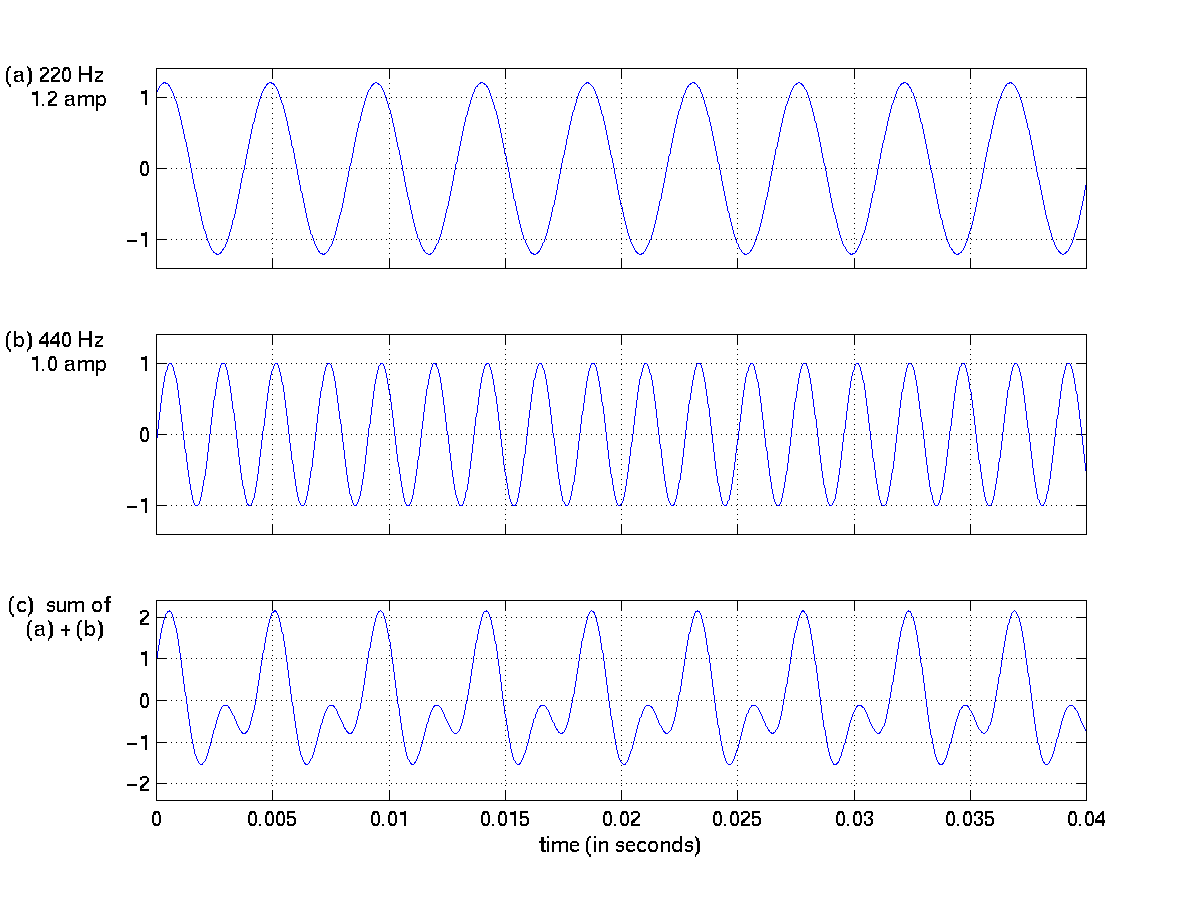
\includegraphics[width=120mm, height=70mm]{\HOME/figures/Synthesis1}
} % end ifthenelse
\caption{Synthesis by addition of two pure sine waves, (a)+(b)=(c).}
\label{fig:synth1}
\end{figure}

The technique of expressing a function as a sum of sinusoidal
components has been around for at least 200 years.  It is important
not only for our analytic understanding of sound waves, but also for
understanding the human perception of sounds.  It is believed that the 
ear functions as a kind of biological spectrum analyzer.  That is,
when sound waves impinge on the ear, what we perceive is a direct
result of the spectral components of the sound, and is only indirectly
a result of the composite waveform.

%% (begin: included from file phase.tex)
Take the wave forms in Figure~\ref{fig:synth1} for example.  Our eardrum
vibrates under the influence of the composite wave appearing in part (c).
However, the mechanisms of the inner ear -- our spectrum analyzer --
enable us to perceive the sound more precisely as a composition of (a)
and (b).  In Figure~\ref{fig:synth2}, sine wave (b) is still
modulating at 440 Hz, but it now begins at a different phase.
Therefore, the composite wave form shown in part (c) of
Figure~\ref{fig:synth2}, has a very different shape than that of
Figure~\ref{fig:synth1}. Yet the human ear perceives the same sound,
since both waves comprise the same frequency components.  
\begin{figure}
\ifthenelse{\boolean{nofigures}}{}{
%             \pdfimage
%             width 120 mm %             width 13 cm
%             height 70 mm %             height 10 cm
%             {\HOME/figures/Synthesis2.png}
\centering  
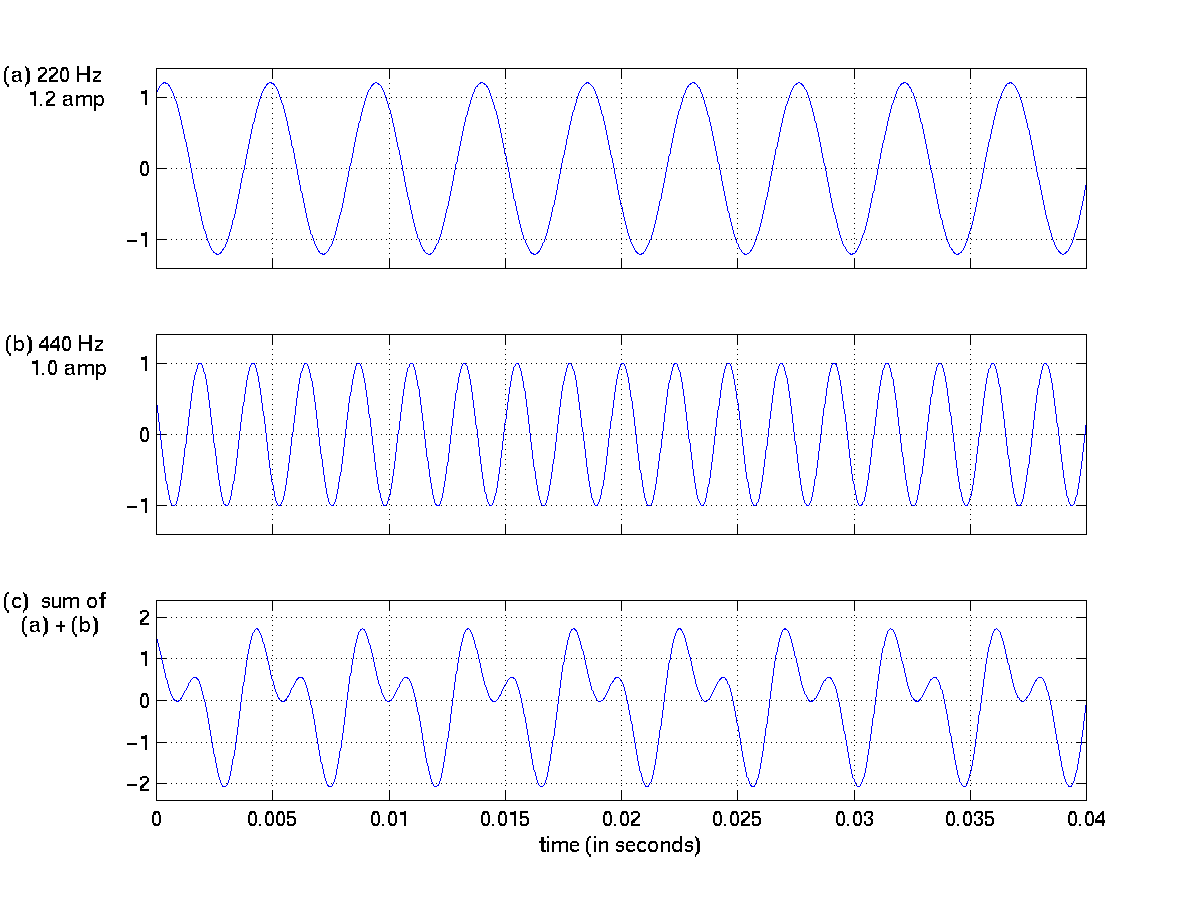
\includegraphics[width=120mm, height=70mm]{\HOME/figures/Synthesis2}
}
\caption{Synthesis by adding sine waves having the same frequencies as
those of Figure~\ref{fig:synth1}, but now the phase of sine wave (b) has
been shifted. Though waveform (c) looks different from that of
Figure~\ref{fig:synth1}, the same sound is perceived.}
\label{fig:synth2}
\end{figure}
%% (end: included from file phase.tex)

The foregoing presents a very basic idea underlying the formation of the
complex tone, $x(t)$.  It can be expressed mathematically as
\begin{equation}
\label{eqn:sumcos}
x(t) = \sum_{k=1}^K a_k \cos(\omega_k t + p_k)
\end{equation}
where the $a_k$ define the amplitudes associated with each partial and
the $p_k$ are some (usually arbitrarily specified) phases.  For
example, the figures above represent the function
\[x(t) = 1.2 \cos(220 t + p_1) + 1.0 \cos(440 t + p_2)\]
for $0 < t \leq (0.04)2\pi $ and $0 < p_k \leq 2\pi$.

The relevance of expression (\ref{eqn:sumcos}) for the analysis of
music is limited by the fact that real world signals, unlike those in
the figures, are never exactly periodic.  Strong similarities among
segments of signals often occur, which give rise to a sense of
pseudo-periodicity and, hence, pitch. However, superimposed on this
periodicity are fluctuations, noise, small frequency variations, etc.
These aperiodic components are due to different phenomena connected
with the particular physical mechanism used for the production of the
sound under analysis (Cavaliere and Piccialli).  For this reason, a
realistic model of a signal must generalize this simple,
time-invariant addition of periodic sine waves.  It should allow both
the amplitudes and frequencies to vary with time.  Writing 
$a_k = a_k(t)$ and $\omega_k t + p_k = \phi_k(t)$ accomplishes this
and yields the 
%following signal plus noise statistical model:
following sum of partials:
\begin{equation}
\label{eqn:sumpartials}
%y(t) = f[t|\beta(t)] + \epsilon(t), \mbox{ with }
x[t|\beta(t)] = \sum_{k=1}^K a_k(t) \cos(\phi_k(t))
\end{equation}
where the notation $x(\cdot|\beta)$ indicates that the
functional form of $x$ is conditional on the time-varying vector
$\beta(t) \equiv (a_1(t),\ldots,a_K(t),\phi_1(t),\ldots,\phi_K(t))^t$ of
amplitudes and phases.  This model also requires
that $a_k(t)$ and $\phi'_k(t)$ vary slowly~\cite{Rodet:1992}.  This
requirement as well as the relationship between the ``instantaneous
frequency,'' $\omega_k,$ and the time-varying phase, $\phi_k(t),$ will
be discussed in the following sections. 

Still implicit in model~(\ref{eqn:sumpartials}) is the assumption that
the signal is well approximated by a sum of pure sinusoidal waves.  
However, the presence of a given frequency, $\omega_k,$ can now be
short lived, and its contribution to $x$ varies (albeit slowly) with
time via $a_k(t)$.   
%Further, to account for the aperiodic component of the signal, a
%non-sinusoidal noise term, $\epsilon(t)$ appears.  The following
%sub-section describes the assumed functional form of $\epsilon(t)$ as
%well as
%As in Serra~\cite{Serra:1989}, we can take this to be a stationary
%autoregressive process.   

Assuming model (\ref{eqn:sumpartials}), the problem of analyzing a signal
becomes the estimation of $\beta(t),$ and there are as many approaches
to that problem as there are applications of signal analysis.  

In later sections, we consider which signal analysis methods are
particularly well suited to the type of musical analysis we wish to
perform.  Therefore, it is crucial that we have a good grasp of the
musical ideas underlying and motivating our research into musical
signal analysis.  The following section presents one such notion --
musical \emph{consonance}.  Also presented are some existing
quantitative measures of this concept. 
% (end: insert file synthesis.tex)

% (begin: insert file consonance.tex)
\subsection{Consonance and Dissonance}
\label{sec:consonance}
According to Tenney~\cite{Tenney:1988} and Sethares
\cite{Sethares:1997}, the historical usage of the term {\it
consonance} (and its antonym, {\it dissonance}) can be classified
according to five distinct categories.
(see~\cite{Sethares:1997} for more details)
\begin{enumerate}
\item {\bf Melodic Consonance (CDC-1)} successive melodic intervals are
consonance or dissonant depending on the surrounding melodic context;
refers to relatedness of pitches sounded successively (melodic contour)
\item {\bf Polyphonic Consonance (CDC-2)} consonance is a function of
the interval between (usually 2) simultaneously sounding tones;
proponents of this definition are clearest about the consonant
$\leftrightarrow$ ``pleasant'' association.
\item {\bf Contrapuntal Consonance (CDC-3)} consonance is defined by
its role in counterpoint, e.g.~voice-leading techniques; the 4th is
declared dissonant (in contrast to CDC-2).
\item {\bf Functional Consonance (CDC-4)} focus on relation of
individual tones to the root or tonic; consonant tones are those that
are in simple unison, third, or fifth relation to root.  Dissonance
occurs when the music moves away from root and sets up a desired
return; dissonances cause chordal motion (and not vice-versa);  Piston
in ``Harmony'' relates consonant with stable or complete
and dissonant with restless or requiring resolution; ``the
essential quality of dissonance is its sense of movement and
not...its degree of unpleasantness to the ear.''
\item {\bf Sensory Consonance (CDC-5)}  equates consonance with
smoothness and the absence of beats; equates dissonance with roughness
and the presence of beats.
\end{enumerate}

The definition of sensory consonance is based on the  phenomenon of
beats.  If two pure sine tones are sounded at almost the same
frequency, then beating occurs due to the interference between the
tones.  The beating becomes slower as the two frequencies approach
each other and disappears when they coincide.  Typically, slower  
beats are perceived as gentle and pleasant while fast beats are
perceived as rough and unpleasant. Observing that any sound can be
decomposed into sinusoidal partials, Helmholtz \cite{Helmholtz:1877}
theorized that the perception of dissonance in a musical tone is
determined by the presence and quality of beats among the tone's
interacting partials. 

The present research effort is directed at the discovery of a
definition that might reconcile these competing notions of consonance.
In particular, we  would like to exploit the theory of \emph{sensory}
and \emph{tonal} consonance (CDC-2 and CDC-5)
of Plomp and Levelt~\cite{Plomp:1965} as well as its elaboration
in~\cite{Sethares:1997}.  Some of this theory is described below in
section~\ref{sec:disscurves}.  Briefly, it employs functions called
\emph{dissonance curves} which measure the ``sensory'' dissonance, of
a complex tone at each particular instant in time.\footnote{Really, a
small interval of time is required to ascertain what (pseudo-)periodic
frequencies are present at a particular instant.}   
This provides a useful point-wise measure.
However, we would also like a measure that is dynamic and appeals to a
melodic sense of consonance.  For example, a dissonance curve does not
account for dissonance due to melodic changes from one complex tone to
the next.  

\subsection{Dissonance Curves}
\label{sec:disscurves}
Two pure sine waves are both perceptible if the frequencies are well
separated.  When the frequencies are close together, only one sine
wave is heard (though possibly with beats).  By varying the frequency
of one of the waves while keeping the other wave fixed, Plomp and
Levelt~\cite{Plomp:1965} gathered data revealing subject's preferences
for various frequency intervals.  An example of what these data
indicate appears as a \emph{dissonance curve} in 
Figure~\ref{fig:1DissCurve}.  (One method of deriving such curves in
practice is described in section~\ref{sec:FourierDissonance}.)  The
curves in the figure are in stark contrast to existing musical theory.
In particular they imply that, in terms of sensory dissonance,
intervals such as the major 7th and minor 9th are almost
indistinguishable from the octave.  This leads some to argue that
these data bear no relation to our notions of musical
consonance. Regardless of whether they have a direct influence on our
ideas about musical intervals, dissonance curves provide a way to
measure the intervals among \emph{pure sine waves}.  Therefore, they
can be useful when analyzing a musical signal that has been decomposed
into its spectral components.

\begin{figure}
\ifthenelse{\boolean{nofigures}}{}{
\centering  
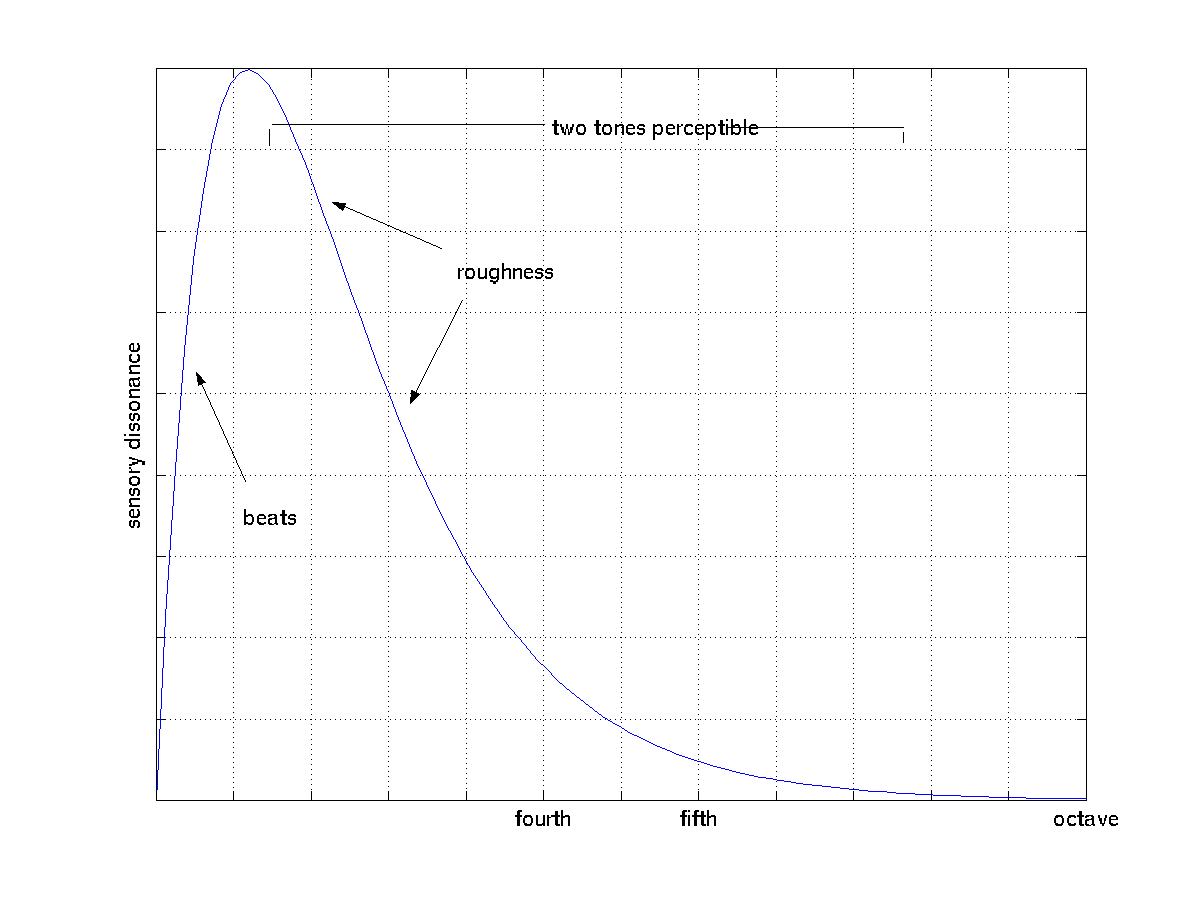
\includegraphics[width=120mm, height=70mm]{\HOME/figures/1DissCurve}
}
\caption{{\small Two sine waves are sounded simultaneously.  Typical
perceptions include pleasant beating (at small frequency ratios),
roughness (at middle ratios), and separation into two tones (at first
with roughness, and later without) for larger ratios.  the horizontal
axis represents the frequency interval between the two sine waves,
and the vertical axis is a normalized measure of ``sensory''
dissonance.  The frequency of the lower sine wave is 400 Hz}}
\label{fig:1DissCurve}
%\end{figure}
%\begin{figure}
\ifthenelse{\boolean{nofigures}}{}{
%             \pdfimage
%             width 120 mm 
%             height 70 mm
%             {\HOME/figures/3DissCurves.png}
\centering  
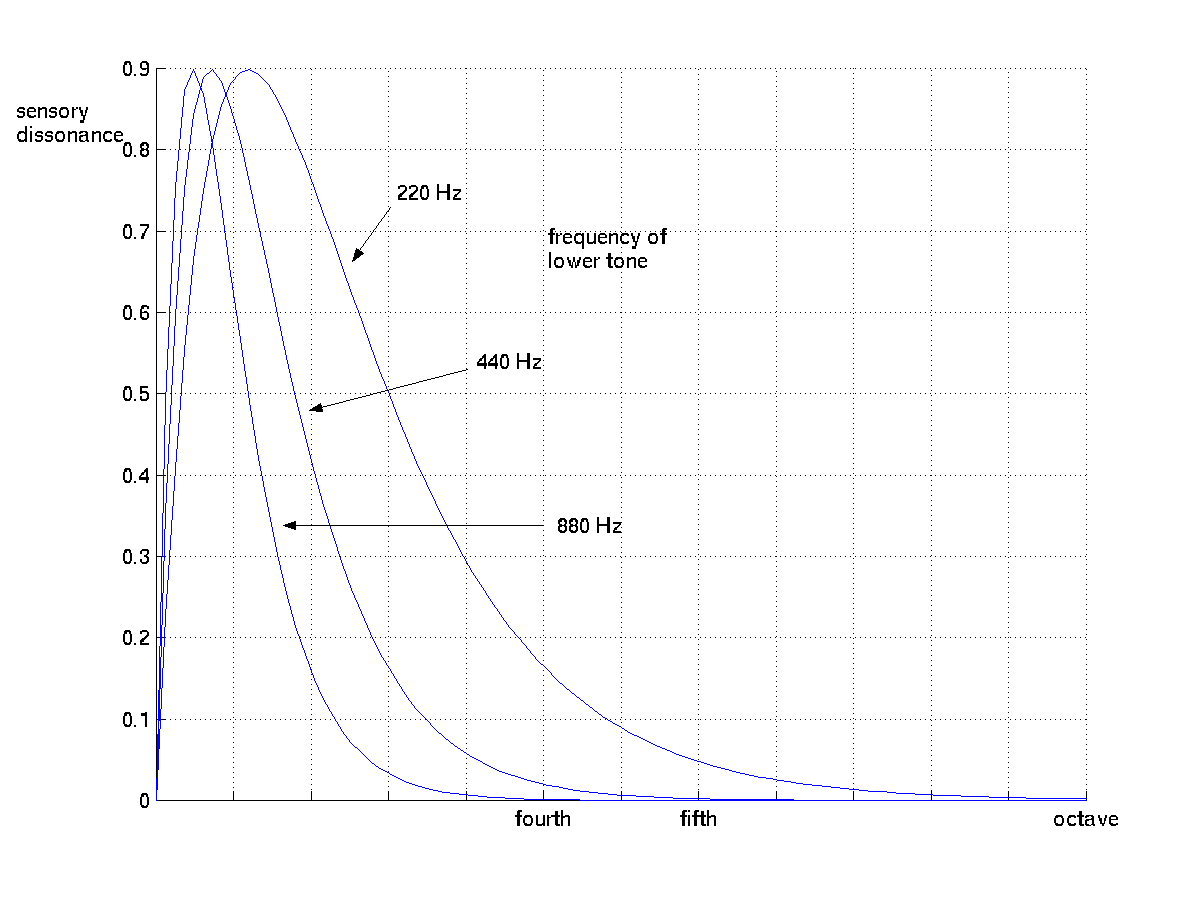
\includegraphics[width=120mm, height=70mm]{\HOME/figures/3DissCurves}
}
\caption{{\small Two sine waves are sounded simultaneously.  The
horizontal axis represents the frequency interval between the two sine
waves, and the vertical axis is a normalized measure of ``sensory''
dissonance. The plot shows how the sensory consonance and dissonance
change depending on the frequency of the lower tone.}}
\label{fig:3DissCurves}
\end{figure}
% (end: insert file consonance.tex)

%%% NEWER (UNDERDEVELOPED) IDEAS %%%
%Recall equation~(\ref{eqn:sumpartials}) of section~\ref{sec:synthesis}
%in which a complex tone $x$ is modeled as a weighted sum of sinusoidal
%partials: 
%\[x(t) = \sum_{k=1}^K a_k(t) \cos(\phi_k(t))\]
%where the instantaneous frequency of the $k$th partial is
%%(cf.~\S~\ref{sec:instfreq}, equation~\ref{eqn:sumpartials}): 
%\[\omega_k(t) = \phi'_k(t) \geq 0.\]
%Suppose for simplicity that the set of $K$ instantaneous frequencies
%$\{\omega_k\}$ are known and constant over a small interval (instant)
%of time.  Then...
%%the relative dissonances among the frequencies in a complex
%%tone
%
%It is possible that a particular \emph{instant} in a piece of music
%will have a high sensory dissonance value but, because of this
%instant's relation to its context, the section of the piece containing
%this instant has a low total dissonance value.  We can create measures
%that act in this way.  Consider a simple succession of 3 instants of a
%musical piece represented by $\{S_0, S_1, S_2\}.$  Let $\|\cdot\|$ be
%the measure of dissonance of $S_k.$  It is possible ...


% -*- mode: LaTeX; tex-main-file: "../Notes.tex"; -*-
\section{Atomic Decompositions}
\label{sec:atomic}
\ifthenelse{\boolean{nofootnotes}}{\subsection{Time-Frequency Atoms}}
{\subsection{Time-Frequency Atoms\protect\footnotemark}
\footnotetext{Mallat~\cite{Mallat:1998} (p.67)}}
A linear time-frequency transform correlates the signal $x$ with a family of
waveforms that are well concentrated in time and in frequency.  These
waveforms are called \emph{time-frequency atoms}. Let us consider a general
family of time-frequency atoms  $\{\phi_{\gamma}\}_{\gamma \in \Gamma}$, 
where $\gamma$ might be a multi-index parameter.  We suppose that
$\phi_{\gamma} \in \LtwoR$ and that $\|\phi_{\gamma}\|=1$.  The
corresponding linear time-frequency transform of $x\in \LtwoR$ is defined
by  
%\begin{eqnarray*}
\begin{alignat}{2}
\T[x](\gamma)   &=\langle x,\phi_{\gamma} \rangle
                &&=\integral x(t)\phi^*_{\gamma}(t)\,dt \nonumber \\
\label{eqn:TFTF}&=\langle X,\Phi_{\gamma} \rangle
                &&=\integral X(\omega)\Phi^*_{\gamma}(\omega)\,d\omega 
\end{alignat}
The third equality holds by the Parseval formula (\ref{sec:Parseval}).

If $\phi_{\gamma}(t)$ is approximately zero when $t$ is outside a
neighborhood of an abscissa $u$, then  
$\langle x,\phi_{\gamma}\rangle$ 
depends only on the values of $x(t)$ in this neighborhood.  Similarly,
if  $\Phi_{\gamma}(\omega)$ is negligible for $\omega$ outside a
neighborhood of $\xi$, then~(\ref{eqn:TFTF}) shows that  
$\langle x,\phi_{\gamma} \rangle$ characterizes $X(\omega)$ in that
neighborhood. 

\renewcommand{\thedefine}{}
\begin{define}{\bf Energy Density. }
Suppose that for any point $(u,\xi)$ in the time-frequency plane there
exists a unique atom $\phi_{\gamma(u,\xi)}$ centered at this point.
The time-frequency support of  
$\phi_{\gamma(u,\xi)}$ 
specifies a neighborhood of $(u,\xi)$ where the energy of $x$ is
measured by 
\begin{align} \label{eqn:energy}
E_{\T[x]}(u,\xi) &=\left|\T[x](\gamma)\right|^2 \\
 &=\left|\langle x,\phi_{\gamma(u,\xi)}\rangle\right|^2 \nonumber
% &=\left|\integral x(t) \phi^*_{\gamma(u,\xi)}(t) \,dt\right|^2\nonumber
\end{align}
\end{define}
Later we will see that any such energy density is an averaging of the
\emph{Winger-Ville transform}, with a kernel that depends on the
atoms $\phi_{\gamma}$.

% (begin: inserted from windowedFT.tex)
\ifthenelse{\boolean{nofootnotes}}{\subsection{Windowed Fourier Transform}}
{\subsection{Windowed Fourier Transform\protect\footnotemark}
\footnotetext{Mallat~\cite{Mallat:1998} (p.69)}}
In 1946 Gabor~\cite{Gabor:1946} introduced windowed Fourier atoms to
measure the ``frequency variations'' of sounds.  A real and symmetric
window $g(t)=g(-t)$ is translated by $u$ and modulated by the
frequency $\xi$:
\[g_{u,\xi}(t) = e^{i2\pi\xi t}g(t-u)\]
The original window, $g$, has unit norm and therefore $\|g_{u,\xi}\|=1$
for any $(u,\xi)\in \R^2$.  The resulting windowed Fourier transform
of $x\in \LtwoR$ is 
\begin{eqnarray}\label{eqn:WindowedFT}
  \S[x](u,\xi) 
  &=& \langle x(t),g_{u,\xi} \rangle \nonumber\\
  &=& \integral x(t)g(t-u) e^{-i2\pi \xi t}\,dt
\end{eqnarray}
This transform is also called the \emph{short time Fourier transform}
because the multiplication by $g(t-u)$ localizes the Fourier integral
in the neighborhood of $t=u$.

As in~(\ref{eqn:energy}), one can define an energy density, called a
\emph{spectrogram}, by
\begin{align*}
  E_{\S[x]}(u,\xi)  &= \left|\S[x](u,\xi)\right|^2\\
  &= \left|\langle x(t),g_{u,\xi}\rangle\right|^2 
%  &= \left|\integral x(t) g(t-u) e^{-i2\pi\xi t}\,dt\right|^2\\
\end{align*}
The spectrogram measures the energy of $x$ in the time-frequency
neighborhood of $(u,\xi)$ specified by the Heisenberg box of
$g_{u,\xi}$. 
% (end: inserted from windowedFT.tex)

% (begin: inserted from wavelet.tex)
\ifthenelse{\boolean{nofootnotes}}{\subsection{Wavelet Transforms}}
{\subsection{Wavelet Transforms\protect\footnotemark}
\footnotetext{Mallat~\cite{Mallat:1998} (p.79)}}
\label{sec:atom-decomp}
To analyze signal structures of very different sizes, it is necessary
to use time frequency atoms with different time supports.  The wavelet
transform decomposes signals over dilated and translated wavelets.  A
wavelet is a function $\psi \in \LtwoR$ with zero average:
\[ \integral \psi(t)dt = 0\]
It is normalized, $\|\psi\|=1$ and centered in the neighborhood
$t=0$.  A family of time-frequency atoms is obtained by scaling $\psi$
by $s$ and translating it by $u$:
\[\psi_{u,s}(t) = \scale \psi \transcale\]
These atoms remain normalized: $\|\psi_{u,s}\|=1$.  The wavelet
transform of a function $x\in \LtwoR$ at time $u$ and scale $s$ is:
\begin{equation}
\label{eqn:wavelet}
\W[x](u,s) = \langle x,\psi_{u,s}\rangle
= \integral x(t)\scale \psi^* \transcale dt
\end{equation}

Like a windowed Fourier transform, a wavelet transform can measure the
time evolution of frequency transients.  This requires using a complex
analytic wavelet, which can separate amplitude and phase components.
An analytic wavelet can be used to measure \emph{instantaneous
frequencies}.  In contrast, real wavelets are often used to detect
sharp signal transitions.

\ifthenelse{\boolean{nofootnotes}}{\begin{define}{\bf Analytic Signals. }}
{\begin{define}{\bf Analytic Signals.\protect\footnotemark }
\footnotetext{Mallat~\cite{Mallat:1998} (p.84)}}
To analyze the time evolution of frequency tones, it is necessary to
use an analytic wavelet to separate the phase and amplitude
information of signals.
%\renewcommand{\thedefine}{}
%\begin{define}
%{\bf Analytic Signal. }
A function $x_a \in \LtwoR$ is said to be \emph{analytic} if its
Fourier transform is zero for negative frequencies:
\[X_a(\omega) = 0 \text{ if } \omega < 0.\]
\end{define}
An analytic function is necessarily complex but is entirely
characterized by its real part.  Indeed, the Fourier transform of its
real part $x = \Real[x_a]$ is 
\[X(\omega) = \frac{X_a(\omega) +
X^*_a(-\omega)}{2}\]
and this relation can be inverted to yield
\begin{equation}
\label{eqn:analFT}
X_a(\omega) = 
    \left\{ \begin{array}{lr}
        2X(\omega)& \text{ if } \omega \geq 0\\
        0 & \text{ if } \omega < 0
        \end{array} 
    \right.
\end{equation}
The analytic part $x_a(t)$ of a signal $x(t)$ is the inverse Fourier
transform of $X_a(\omega)$ defined by~(\ref{eqn:analFT}).

Equivalently, we obtain the analytic part of $x(t)$ a signal by
operating on the signal with the \emph{Hilbert transform}.  Precisely,
given a real signal $x(t)$, the analytic part is 
\[
x_a(t) = x(t) + i \H[x](t) = x(t) 
   + \frac{i}{\pi} \pv \integral \frac{x(s)}{t-s} ds
\]
where $\H$ denotes the Hilbert transform.  

\begin{define}{\bf Time-Frequency Resolution. }
% Mallat:1998} (p.85)
An analytic wavelet transform is calculated with an analytic wavelet
$\psi$ with the integral~(\ref{eqn:wavelet}). Its time-frequency
resolution depends on the time-frequency spread of the wavelet atoms  
$\psi_{u,s}$.  
\end{define} 
We suppose that $\psi$ is centered at 0, which implies that 
$\psi_{u,s}$ 
is centered at $t=u$.  
As shown in~\cite{Mallat:1998} (p.~85), the spread with respect to
time is $s^2 \sigma^2_t$, where $\sigma^2_t=\int t^2|\psi(t)|^2 dt$ is
the variance of $\psi$.  Since $\psi$ is analytic, 
$\Psi (\omega)$ 
is zero at negative frequencies, so the center frequency of
$\Psi $ is 
\[\eta =\int_0^{+\infty}\omega|\Psi (\omega)|^2 d\omega\]
The Fourier transform of $\psi_{u,s}$ is a dilation of $\Psi $ by
$1/s$:
\def\waveletFT{\Psi_{u,s}} 
\def\waveletFTomega{\Psi_{u,s}(\omega)} 
\[\waveletFTomega = \sqrt{s}\Psi (s\omega)e^{-i2\pi \omega
u}\]
Its center frequency is therefore $\eta/s$.  The energy spread of
$\waveletFT$ around $\eta/s$ is $\sigma^2_{\omega}/s^2$
(\cite{Mallat:1998} {\it ibid.}). 

Thus the energy spread of a wavelet time-frequency atom $\psi_{u,s}$
corresponds to a Heisenberg box centered at $(u, \eta/s)$, of size
$s\sigma_t$ along time and $\sigma_{\omega}/s$ along frequency.  The
area of the rectangle remains equal to $\sigma_t\sigma_{\omega}$ at
all scales, but the resolution in time and frequency depends on $s$.
As $s$ increases (resp.~decreases) frequency resolution increases
(resp.~decreases) while time resolution decreases (resp.~increases).
%as follows:\\ 
%\begin{center}
%\begin{tabular}{l|l|l}
%scale $s$ & increases & decreases\\
%\hline
%center frequency $\eta/s$ & decreases & increases \\
%frequency spread $\sigma_{\omega}/s$ & decreases & increases \\
%frequency resolution & improves & deteriorates \\
%time spread $s \sigma_t$ & increases & decreases \\
%time resolution & deteriorates &improves
%\end{tabular}
%\end{center}

An analytic wavelet transform defines a local time-frequency energy
density $E_{\W[x]}$, which measures the energy of $x$ in the Heisenberg box
of each wavelet $\psi_{u,s}$ centered at $(t, \xi)=(u, \eta/s)$:
\begin{equation}\label{eqn:energyDensity}
E_{\W[x]}(t,\xi) = \left|\W[x](u,s)\right|^2 =
\left|\W[x]\left(u,\frac{\eta}{\xi}\right)\right|^2
\end{equation}
This energy density is called a \emph{scalogram}.
% (end: inserted from wavelet.tex)

% (begin: inserted from instantfreq.tex)
\ifthenelse{\boolean{nofootnotes}}{\subsection{Instantaneous Frequency}}
{\subsection{Instantaneous Frequency\protect\footnotemark}
\footnotetext{Mallat~\cite{Mallat:1998} (p.91)}}
\label{sec:instfreq}
A cosine modulation 
\[
x(t) = a(t) \cos(\omega_0 t + \phi_0) 
= a(t) \cos\phi(t), \quad \text{ for } a(t) \geq 0
\]
has a frequency $\omega_0$ that is the derivative of the phase
$\phi(t) = \omega_0 t + \phi_0$.  The {\it instantaneous frequency} is
defined as a positive derivative of the phase:
\begin{equation}
\label{eqn:instfreq}
\omega(t) = \phi'(t) \geq 0.
\end{equation}
By adapting the sign of $\phi(t),$ the derivative can be taken to be
positive.  Since there are many possible choices of $a(t)$ and
$\phi(t),$ it is clear that $\omega(t)$ is not uniquely defined
relative to $x$. 

Recall that 
%\begin{define}{\bf Analytic Signal} (\cite{Mallat:1998} p.~84)
a function $x_a \in \LtwoR$ is said to be \emph{analytic} if its
Fourier transform is zero for negative frequencies:
\[X_a(\omega) = 0 \text{ if } \omega < 0.\]
%\end{define}
%\end{definition}
An analytic function is necessarily complex but is entirely
characterized by its real part, $x = \Real[x_a]$, which has the
Fourier transform
\[X(\omega) = \frac{X_a(\omega) +
X^*_a(-\omega)}{2}\]
and this relation can be inverted to yield
\begin{equation}%\label{eqn:analFT}
X_a(\omega) = 
    \left\{ \begin{array}{ll}
        2 X(\omega),& \quad \text{ if } \omega \geq 0\\
        0, & \quad \text{ if } \omega < 0
        \end{array} 
    \right.
\end{equation}
The analytic part $x_a(t)$ of a signal $x(t)$ is the inverse Fourier
transform of $X_a(\omega)$ defined by~(\ref{eqn:analFT}).
Writing the analytic part of $x$ as the modulus times the complex
exponential,
\[x_a(t) = a(t)\exp[i\phi(t)] = a(t)[\cos\phi(t) + i \sin\phi(t)]\]
it is clear that 
\[x(t) = \Real[x_a] = a(t)\cos\phi(t)\]
The factor $a(t)$ is the \emph{analytic} amplitude of $x(t),$ while
$\phi'(t)$ is the instantaneous frequency.  Both $a(t)$ and $\phi'(t)$
are uniquely defined. 

% Mallat:1998 (p.92)
\begin{example}\protect\footnotemark
\footnotetext{Mallat~\cite{Mallat:1998} (p.92)}
If $x(t) = a(t)\cos(\omega_0 t + \phi_0)$, then 
\begin{equation}\label{eqn:CosineFT} 
X(\omega)=
\frac{1}{2}\left(\hat{a}(\omega - \omega_0) e^{i \phi_0} + 
\hat{a}(\omega + \omega_0) e^{-i \phi_0} \right)
\end{equation}
where $\hat{a}(\omega)$ denotes the \FT\ of $a(t)$.
If the variations of $a(t)$ are slow compared to the period $T =
2\pi/\omega$, which is achieved by requiring that the support of
$\hat{a}$ be included in $[-\omega_0,\omega_0]$, then the second term
on the right of~(\ref{eqn:CosineFT}) is zero for $\omega>0$ and 
\[X_a(t) = \hat{a}(\omega - \omega_0) e^{i \phi_0}\]
by~(\ref{eqn:analFT}).  So $x_a(t) = a(t)\exp[i(\omega_0t+\phi_0)]$.
\end{example}

\begin{example} If a signal $x$ is the sum of two sinusoidal waves, 
$a\cos(\omega_1t) + a\cos(\omega_2t)$, then 
\begin{eqnarray*}
x_a(t)&=&a e^{i \omega_1t} + a e^{i \omega_2t}\\
&=& a\cos[ (\omega_1-\omega_2)t/2]\exp[i (\omega_1+\omega_2)t/2]
\end{eqnarray*}
The instantaneous frequency is $\phi'(t)=(\omega_1+\omega_2)/2$ and
the amplitude is 
\[
a(t)= a \left|\cos[ (\omega_1-\omega_2)t/2]\right|
\]
This result is not satisfying because it does not reveal that the
signal includes two sinusoidal waves of the same amplitude.  It
measures an average frequency value.  The next sections explain how to
measure the instantaneous frequencies of several spectral components
by separating them with a windowed Fourier transform or a wavelet
transform. 
\end{example}
% (end: inserted from instantfreq.tex)

% (begin: inserted from ridges.tex)
\ifthenelse{\boolean{nofootnotes}}{\subsection{Fourier Ridges}}
{\subsection{Fourier Ridges\protect\footnotemark}
\footnotetext{Mallat~\cite{Mallat:1998} (p.94)}}
% Mallat:1998 (p.94)
The spectrogram $E_{\S[x]}(u,\xi)$ measures the energy of $x$ in a
time-frequency neighborhood of $(u,\xi)$.  The ridge algorithm
computes the instantaneous frequencies from the local maxima of
$E_{\S[x]}(u,\xi)$.  This approach was introduced by Delprat, Escudi\'{e},
Guillemain, Kronland-Martinet, Tchamitchian and
Torr\'{e}sani~\cite{Delprat:1992} to analyze musical sounds.  Since
then, it has found applications for a wide range of signals that have
time varying frequency tones.

% Mallat:1998 (p. 98)
When the signal contains several spectral lines \emph{whose
frequencies are sufficiently apart}, the windowed Fourier transform
separates each of these components and the ridges detect the evolution
in time of each spectral component.
%\footnote{Mallat~\cite{Mallat:1998} (p.98)}

%% (begin: included from icassp file windowedFT.tex)
The windowed Fourier transform is computed with a symmetric window
$g(t)=g(-t)$ with support $t\in[-1/2,1/2]$ and unit norm, $\|g\|=1$.  
For a fixed scale $s$, $g_s(t)=s^{-1/2}g(t/s)$ has a support of size
$s$ and unit norm.  The corresponding windowed Fourier atoms are 
$g_{s,u,\xi}(t)=g_s(t-u)e^{i \xi t}$
and the windowed Fourier transform is defined by 
\[
\S[x](u,\xi) =\integral x(t)g_s(t-u)\e^{-i \xi t}dt
\]

If $x(t)=a(t)cos\phi(t)$, then the transform $\S[x](u,\xi)$
has the following relation to the instantaneous frequency of $x$:
\begin{equation}
\label{eqn:freqest}
\S[x](u,\xi)=\frac{\sqrt{s}}{2}a(u)\exp(i[\phi(u)-\xi u])
            \left(\hat{g}(s[\xi-\phi'(u)])+\epsilon\right)%\epsilon_{u,\xi}\right)
\end{equation}
for all $\xi \geq 0$.  For bounds on $\epsilon$,
see Mallat~\cite{Mallat:1998}.  Delprat \emph{et al.} \cite{Delprat:1992}
prove a similar result for Gaussian $g$.

If we can neglect the corrective term ($\epsilon$) %$\epsilon_{u,\xi}$,
then~(\ref{eqn:freqest}) enables us to measure $a(u)$ and $\phi'(u)$
using $\S[x](u,\xi)$.  Briefly, the corrective term is negligible when two
conditions are satisfied.
First, let the bandwidth of $\hat{g}$ be $\Delta \omega$ such that 
$|\hat{g}(\omega)|\ll 1$ when $|\omega| \geq \Delta \omega$. 
Then we require that 
\[
\phi'(u) \geq \frac{\Delta \omega}{s}
\]
The second condition permitting us to neglect $\epsilon$ %$\epsilon_{u,\xi}$ 
is
that $a(t)$ and $\phi'(t)$ must have small relative variations over the
support of the scaled window $g_s$.  
If these two conditions are met, then~(\ref{eqn:freqest}) shows that
for each $u$, the spectrogram $\left|\S[x](u,\xi)\right|^2$ is maximized at
$\xi(u)=\phi'(u)$.  The corresponding time-frequency pairs
$(u,\xi(u))$ are called \emph{ridge points}.  
Such points indicate that the predominant spectral components of the
signal occur at frequencies $\phi'(u)=\xi(u)$ with analytic
amplitudes, computed from~(\ref{eqn:freqest}), 
\[
a(u) = \frac{2\left|\S[x](u,\xi(u)\right|}{\sqrt{s}|\hat{g}(0)|}
\]

% Mallat:1998 (p. 98)
When the signal contains several spectral lines \emph{whose
frequencies are sufficiently apart}, the windowed Fourier transform
separates each of these components and the ridges detect the evolution
in time of each spectral component.  Suppose, for instance, that $x$
has the form 
\[
x(t) = a_1(t)\cos\phi_1(t) + a_2(t)\cos\phi_2(t)
\]
where $a_k(t)$ and $\phi'_k(t)$ have small variations over intervals
of size $s$ and $s\phi'_k(t)\geq\Delta\omega$.  Since the Fourier
transform is a linear operation, equation~(\ref{eqn:freqest}) implies
that 
%\begin{eqnarray}
\begin{equation}
\label{eqn:2ridges}
\S[x](u,\xi)\approx\frac{\sqrt{s}}{2}
a_1(u)\exp(i[\phi_1(u)-\xi u])\hat{g}(s[\xi-\phi_1'(u)])%\nonumber \\
\end{equation}
\[+\frac{\sqrt{s}}{2}
a_2(u)\exp(i[\phi_2(u)-\xi u])\hat{g}(s[\xi-\phi_2'(u)])\]
%\end{eqnarray}
The two spectral components can be discriminated if for all $u$,
$\hat{g}(s|\phi'_1(u)-\phi'_2(u)|) \ll 1$
%\[\hat{g}(s|\phi'_1(u)-\phi'_2(u)|) \ll 1\]
which means that the frequency difference is larger than the bandwidth
of $\hat{g}(s\omega)$:
\begin{equation}
\label{eqn:cond}
|\phi'_1(u)-\phi'_2(u)|\geq \frac{\Delta \omega}{s}
\end{equation}
In this case, when $\xi = \phi'_1(u)$, the second term
of~(\ref{eqn:2ridges}) can be neglected and the first term generates a
ridge point from which we may recover $\phi'_1(u)$ and $a_1(u)$.
Similarly for the case $\xi = \phi'_2(u)$.  The ridge points are
distributed along two time-frequency lines $\xi(u)=\phi'_1(u)$ and 
$\xi(u)=\phi'_2(u)$.  This result is valid for any number of
time-varying spectral components, as long as the distance between any
two instantaneous frequencies satisfies~(\ref{eqn:cond}).  For those
values of $u$ at which the spectral lines are too close, they
interfere and destroy the ridge pattern.

\begin{center}
\begin{figure}
\ifthenelse{\boolean{nofigures}}{}{
%	\pdfimage
%        width 120 mm 
%        height 70 mm
\centering
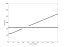
\includegraphics[width=120mm, height=70mm]{\HOME/figures/PureLin440Ridges}
}
\caption{The local maximum moduli of the spectrogram are the ridge
points that locate instantaneous frequencies.}
\label{fig:ridges}
\end{figure}
\end{center}
%% (end: included from icassp file windowedFT.tex)

Figure~\ref{fig:ridges} displays the ridges computed from the local
maxima of the spectrogram of
\begin{equation}
\label{eqn:purelin440}
x(t) = 0.5\cos(2\pi440t) + 0.4\cos(2\pi\alpha440t)
\end{equation}
where $\alpha = 0.5 + 1.5t$.  That is, the first summand is a pure 440 
Hz tone with a constant amplitude of 0.5, while the second term 
has amplitude 0.4 and a frequency that increases linearly from 220 Hz
to 880 Hz over the interval $t\in [0,1]$.  The ridges fail to
accurately describe the frequency content of the signal when $t$
ranges from about 0.3 to 0.4 seconds.  Here the instantaneous
frequencies are too close and the frequency resolution is not
sufficient to distinguish them.

\ifthenelse{\boolean{nofootnotes}}{\begin{define}{\bf Wavelet Ridges. }}
{\begin{define}{\bf Wavelet Ridges.\protect\footnotemark }
\footnotetext{Mallat~\cite{Mallat:1998} (p.102)}}
Windowed Fourier atoms have a fixed scale and thus cannot follow
the instantaneous frequencies of rapidly varying events such as
hyperbolic chirps.  In contrast analytic wavelet transform modifies
the scale of its time-frequency atoms.  The ridge algorithm of Delprat
{\it et al} ({\it op.~cit.}) can be extended to analytic wavelet
transforms to accurately measure frequency tones that are rapidly
changing at high frequencies.
\end{define}
% (end: inserted from ridges.tex)

\subsection{Matching Pursuit}
%\ifthenelse{\boolean{nofootnotes}}{\subsection{Matching Pursuits}}
%{\subsection{Matching Pursuits\protect\footnotemark}
%\footnotetext{Gribonval, {\it et~al}~\cite{Gribonval:1996}}}
\label{sec:MP}
A \emph{matching pursuit}~\cite{Mallat:1993} is an iterative algorithm
that decomposes the signal over \emph{dictionary} vectors.
A dictionary is a family of vectors 
$\mathcal{D}= \{g_\gamma\}_{\gamma\in\Gamma}$ 
included in a Hilbert space $\Hilbert$, with a unit norm
$\|g_\gamma\|=1$.  Such a family can be constructed by scaling,
translating and modulating a single window function $g(t) \in \LtwoR$.
We suppose that $g(t)$ is real, continuously differentiable and
$O(\frac{1}{t^2+1})$.  We further impose that $\|g\|=1$, that the
integral of $g(t)$ is non-zero, and that $g(0)\neq 0$.  
For any scale $s$, translation $u$, and frequency modulation $\xi$, we
denote $\gamma = (u,s,\xi)$ and define
\begin{equation}\label{eq:ggamma}
g_\gamma(t) 
= \frac{1}{\sqrt{s}}g\left(\frac{t-u}{s}\right) e^{i2\pi\xi t}
\end{equation}
The index $\gamma$ is an element of the set 
$\mathbf{\Gamma} = \Real \times \Real^+ \times \Real$.  The factor
$1/\sqrt{s}$ normalizes the norm of $g_\gamma$ to 1. If $g(t)$ is
even, which is generally the case, $g_\gamma(t)$ is centered at the
abscissa $u$.  Its energy is mostly concentrated in a neighborhood of
$u$, whose size is proportional to $s$.  Let $\hat{g}(\omega)$ be the
\FT\ of $g(t)$.  Equation~(\ref{eq:ggamma}) yields
\[
\hat{g}_\gamma(\omega) 
= \sqrt{s}\hat{g}(s(\omega - \xi))e^{-i2\pi(\omega-\xi)u}
\]

The matching pursuit algorithm iteratively decomposes a signal over
dictionary vectors as follows.
Let $R^0x(t)=x(t)$, and suppose that we have computed the $n^{th}$
order \emph{residue}, $R^nx$, for $n\geq 0$.  We then choose an
element, $g_{\gamma_n}$ which closely ``matches'' the residue in the
following sense:
\[
|C(R^nx,g_{\gamma_n})| = \sup_{\gamma \in \Gamma} |C(R^nx,g_\gamma)|
\]
where $C(x,g_\gamma)$ is a correlation function which measures the
similarity between $x$ and $g_\gamma$.  An example is the usual inner
product, $\langle x,g_\gamma \rangle$.

Next, decompose the residue as 
\[
R^nx(t) = C(R^nx,g_{\gamma_n})g_{\gamma_n}(t) + C(R^{n+1}x(t)
\]
which defines the residue for step $n+1$, and fully specifies the
algorithm recursion.  

With the usual inner product as the correlation function, it can be
shown (\cite{Mallat:1998}, p.422) that the magnitude of the residue,
$\|R^nx\|$ converges to 0 exponentially as $n$ increases.  This yields
the following atomic signal decomposition:
\begin{equation}\label{eq:MP}
x(t) = \sum_{n=0}^\infty C(R^nx,g_{\gamma_n})g_{\gamma_n}(t) 
\end{equation}



% -*- mode: LaTeX; tex-main-file: "../Notes.tex"; -*-
% (begin: insert file ambiguity.tex)
%\subsection{Quadratic Time-Frequency Energy\protect\footnotemark}
%\footnotetext{Mallat~\cite{Mallat:1998} (p.107),
%Mertins~\cite{Mertins:1999} (p.265)} 
\section{Energy Distributions}
\label{sec:energy}
Wavelet and windowed Fourier transforms are computed by
correlating the signal with families of time-frequency atoms.  The
time and frequency resolution of these transforms is thus limited by
the time-frequency resolution of the corresponding atoms.  Ideally,
one would like to define a density of energy in a time-frequency
plane with no loss of resolution.  This section presents a
different class of time-frequency representation (TFR) which is not
restricted by the uncertainty principle.  

%\footnotetext{Mertins~\cite{Mertins:1999} (p.265)}
The \emph{Wigner-Ville time-frequency representation} is computed by
correlating $x$ with a time and frequency translation of itself.
(Below we refer to the Wigner-Ville TFR simply as the ``\WV'' and,
sometimes, as the ``\WT.'')  Though it yields some remarkable
properties, the quadratic from of this representation can also limit
its application because of the inevitable cross terms that appear in 
quadratic forms.  In such cases, these so-called ``interference
terms'' can be attenuated by a time-frequency averaging, but this
procedure results in a loss of resolution. Below we see that the
spectrogram, the scalogram and all squared time-frequency
decompositions can be written as a time-frequency averaging of the
\WT. 

Although the TFR's of this section do not yield positive
distributions in all cases, they allow extremely good insight into
signal properties within certain applications.  

\ifthenelse{\boolean{nofootnotes}}{\subsection{Ambiguity Function}}
{\subsection{Ambiguity Function\protect\footnotemark}
\footnotetext{Mertins~\cite{Mertins:1999} (p.265)}}
\label{sec:ambig-funct}
This section describes TFR's that are computed by correlating a signal,
$x(t)$, with time and frequency shifted versions of itself.  We start
by looking at time and frequency shifts separately.

\begin{define}{\bf Time-Shifted Signals. }  We define the 
\emph{temporal autocorrelation function}, $r_{x}(\tau)$, by
correlating $x(t)$ with a time translation of itself:
%\begin{align}
\begin{equation}
\label{eqn:autocorrelation} 
r_{x}(\tau) = \langle x_\tau,x \rangle 
             = \integral x(t+\tau)x^*(t)\,dt\\
%&= \integral x(t)x^*(t-\tau)\,dt = \langle x,x_{-\tau} \rangle 
%\end{align}
\end{equation}
\end{define}
A simple change of variable %in (\ref{eqn:autocorrelation}) 
shows that $r_{x}(\tau) = \langle x,x_{-\tau} \rangle$.

The distance $d(x, x_\tau)$ between an energy signal $x(t)$ and its
time-shifted version $x_\tau(t) = x(t+\tau)$ is related to %$r_x(\tau)$ 
the autocorrelation function according to the following equation: 
\[
d(x, x_\tau)^2 = 2\|x\|^2 - 2 \,\Real[r_{x}(\tau)]
\] 

Let $Y(\omega)$ denote the Fourier transform of $y(t)$ and recall the
following correspondences:\\
\begin{center}
\begin{tabular}{l|c|c}
&$y(t)$&$Y(\omega)$\\
\hline
translation & $x(t-t_0)$ & $e^{-i2\pi\omega t_0}X(\omega)$\\
modulation & $e^{i2\pi\omega_0t}x(t)$ & $X(\omega-\omega_0)$\\
conjugation & $x^*(t)$ &$ X^*(-\omega)$
\end{tabular}
\end{center}
\vspace{4mm}
Also, recall Parseval's relation from section~\ref{sec:Parseval}: 
$\langle X,Y\rangle = \langle x,y\rangle$. 
Now, if we put $y(t) = x(t+\tau)$ in
equation~(\ref{eqn:autocorrelation}), it is easy to see that
$r_{x}(\tau) = \langle y,x\rangle = \langle Y,X\rangle$.  More
explicitly, we have 
\begin{eqnarray}
r_{x}(\tau)&=&\integral Y(\omega) X^*(\omega)\,d\omega \nonumber \\
&=&\integral e^{i2\pi\omega\tau}X(\omega) X^*(\omega)\,d\omega\nonumber\\
%&=& \integral S_{x}(\omega)e^{i2\pi \omega \tau}\,d\omega 
&=& \integral  |X(\omega)|^2 \,e^{i2\pi \omega \tau}\,d\omega 
\label{eq:6}
\end{eqnarray}
%where $S_{x}(\omega) = |X(\omega)|^2$ 
where $|X(\omega)|^2$ is the \emph{spectral energy density.}  Thus,
inverting~(\ref{eq:6}), we see that the spectral energy density is the
\FT\ of the temporal autocorrelation function.

\begin{define}{\bf Frequency-Shifted Signals. }  Frequency shifted
versions of a signal $x(t)$ are often produced due to the Doppler
effect.  If we wish to estimate such a frequency shift in order to
determine the velocity of a  moving object, we consider the distance
between a signal $x(t)$ and its frequency-shifted, or
\emph{modulated}, version $x_\xi(t) = x(t)e^{i2\pi\xi t}$. 
The distance is given by
\[
d(x, x_\xi)^2 = 2\|x\|^2 - 2 \,\Real\langle x_\xi,x\rangle
\] 
\end{define}
The foregoing inner product will be denoted $\rho_{x}(\xi)$.  Thus,
\begin{align*}
\rho_{x}(\xi)&= \langle x_\xi,x \rangle 
              = \langle x,x_{-\xi}\rangle\\
             &= \integral e^{i2\pi\xi t} x(t)x^*(t)\,dt\\
%&=& \integral s_{x}(t)e^{i\xi t}\,dt 
             &= \integral |x(t)|^2 \,e^{i2\pi\xi t}\,dt 
\end{align*}
%where $s_{x}(t) = |x(t)|^2$ 
where $|x(t)|^2$ is the \emph{temporal energy density.}  It is also
called the \emph{instantaneous power} of the signal.

It is possible to view $\rho_{x}(\xi)$ as the spectral analog of the
temporal autocorrelation function, $r_{x}(\tau)$, when we write the
former in as a \emph{spectral autocorrelation function.}  That is,
using the Fourier relations reviewed above and the Parseval identity,
% we can write 
\[
\rho_{x}(\xi) = \integral X(\omega - \xi)X^*(\omega)\,d\omega
\]
In other words, $\rho_{x}(\xi)$ is the autocorrelation function of the
spectrum $X(\omega)$.

\begin{define}{\bf Time and Frequency-Shifted Signals. }  
We now consider shifting a signal in both the time and frequency domains
simultaneously.  For this, a transform known as the 
%following transform is often useful.
%\end{define}
%\begin{definition}{\bf Ambiguity Function. } The 
\emph{ambiguity function} plays a central role as the 
\emph{time-frequency autocorrelation function}.  
It is defined as follows: 
\[
\A_{x}(\xi,\tau) = \integral \xtpull \xtpushconj e^{i2\pi \xi t}\,dt
\]
Once again, Parseval provides for the definition as a frequency
integration
%on the frequency domain,  
\[
\A_{x}(\xi,\tau) = \integral \Xtpush \Xtpullconj e^{i2\pi \nu \tau}\,d\nu
\]
\end{define}
Analogous to the cross correlation function is the
\emph{cross ambiguity function} defined by 
\begin{eqnarray}
\label{eqn:crossAmbiguity}
  \A_{xy}(\xi,\tau) 
   &=& \integral \xtpull \ytpushconj e^{i2\pi \xi t}\,dt\\
   &=& \integral \Xtpush \Ytpullconj e^{i2\pi \xi t}\,dt\nonumber \\
\end{eqnarray}
% (end: insert file ambiguity.tex)

At this point it is helpful to summarize what we have shown thus
far.  The functions $r_x(\tau)$ and $\rho_x(\xi)$ are the
autocorrelation functions associated with shifts in time and frequency,
respectively.  The \emph{spectral} energy density is the \FT\ of the
\emph{temporal} autocorrelation function:
\[
\left|X(\nu)\right|^2 = \integral r_x(\tau)e^{-i2\pi\nu\tau}\,d\tau
\]
The \emph{temporal} energy density is the \FT\ of the
\emph{spectral} autocorrelation function:
\[
\left|x(t)\right|^2 = \integral \rho_x(\xi)e^{-i2\pi\xi t}\,d\xi
\]
The spectral and temporal energy densities can be viewed as
``marginal'' energy densities in their respective variables.
The ambiguity function generalizes the ``marginal'' autocorrelation
functions, $r_x(t)$ and $\rho_x(\xi)$, to simultaneously account for
both time and frequency shifts.  
Thus, it is the ``joint'' autocorrelation function.  The
natural next step, then, is to consider the \FT\ of the ambiguity
function.  Perhaps this defines a useful ``joint'' energy density,
with the correct marginal densities, 
$\left|X(\nu)\right|^2$ and $\left|x(t)\right|^2$.  We define such a 
transform in the next section, and relate it to the foregoing
interpretation as a ``joint energy density'' in
section~\ref{sec:wign-ambig-relat}.

% (begin: insert file Wigner.tex)
\ifthenelse{\boolean{nofootnotes}}{\subsection{Wigner Transform}}
{\subsection{Wigner Transform\protect\footnotemark}
\footnotetext{Mertins~\cite{Mertins:1999} (p.265)}}
%\begin{define}{\bf Wigner Transform. } The quadratic form 
The ambiguity function represents the signal energy %of the signal 
in the {\it frequency-time} plane.  We now transform this
representation into the {\it time-frequency} plane.
%The \WV\ transform is also computed by integrating the product of $x$
%with time and frequency translations of itself.  However, the
%variable over which we integrate is now the shift variable.  

The quadratic form
\begin{equation} \label{eqn:WignerVille}
\W_x(t,\nu) = 
\integral \xtpull \xtpushconj e^{-i2\pi \tau\nu}\,d\tau
\end{equation}
is known as the \emph{Wigner-Ville distribution}, or \emph{\WT}.
As we show in the next section, it is the two-dimensional \FT\ of the
ambiguity function.  Also, as the one-dimensional \FT\ of 
$\xtpushconj \xtpull$, which has a Hermitian symmetry in $\tau$, the
\WV\ transform is real valued. 

Time and frequency play a symmetric role, % Mallat:1998 (p.108)
and the transform can be written as a frequency integral by
applying the Parseval formula:
\begin{equation} \label{eqn:WignerVilleF}
\W_x(t,\nu) = %\frac{1}{2\pi}
\integral \Xtpush \Xtpullconj \e^{-i2\pi\xi t}\,dt
%\hat{f}\left(\xi+\frac{\gamma}{2}\right)
%\hat{f}^*\left(\xi-\frac{\gamma}{2}\right)
\end{equation}

%\begin{define}{\bf Time-Frequency Support. }  
The \WV\ transform localizes the time-frequency structures of $x$.  If
the energy of $x$ is well concentrated in time around $t_0$ and in
frequency around $\nu_0$ then $\W_x$ has its energy centered at
$(t_0,\nu_0)$, with a spread equal to the time and frequency spread of
$x$. 
%\end{define}

% Mallat:1998 (p.109)
\begin{define} {\bf Instantaneous Frequency. }
%\footnote{Mallat~\cite{Mallat:1998} (p.109)}
Ville's original motivation for studying time-frequency decompositions
was to compute the instantaneous frequency of a signal.  Assume $x$
has the form $x(t) = a(t)\cos\phi(t)$ and let $x_a$ be the analytic
part of $x$ obtained by setting $X(\nu)=0$ for $\nu < 0$.  Equivalently,
$x_a(t) = a(t)\exp[i\phi(t)]$ so that $x = \Real[x_a]$, and
$\nu=\phi'(t)$ is the instantaneous frequency.  The following
proposition states that $\phi'(t)$ is the ``average'' frequency
computed relative to the transform $\W_x$.
\end{define}
\begin{prop}
If $x_a(t) =  a(t)\exp[i\phi(t)]$, then
\[
  \phi'(t) =
  \frac{\int \nu \W_{x_a}(t,\nu)\,d\nu}
       {\int \W_{x_a}(t,\nu)\,d\nu}
\]
where integration is over all $\R$.
\end{prop}
This proposition shows that, for a fixed $t=t_0$, the mass of
$\W_{x_a}(t_0,\nu)$ is typically concentrated in the neighborhood of the
instantaneous frequency $\nu_0 = \left.\phi'(t)\right|_{t=t_0}$.
% (end: insert file Wigner.tex)

% (begin: insert file WignerAmbiguity.tex)
\subsection{Wigner-Ambiguity Relations}\label{sec:wign-ambig-relat}
%\begin{define} {\bf Wigner-Ambiguity Relations. }
To help further motivate the definition of the \WV, we relate it
%let us consider its relation 
to other entities, about which we might have better intuition.  
First, let us simplify notation by introducing the signals
\begin{equation}\label{eq:8}%alignat}{2}
\xpullpush(t) = \xtpull e^{i2\pi \halfxi t},\qquad 
\xpushpull(t) = \xtpush e^{-i2\pi \halfxi t}%\label{eq:8}
\end{equation}
\begin{equation}\label{eq:9}%alignat}{2}
\ytnu(\tau)  = \xtpull e^{-i2\pi \nu \halftau},\qquad 
\ytnu(-\tau) = \xtpush e^{i2\pi \nu \halftau}%\nonumber\\
\end{equation}
which are time and frequency shifted versions of 
%one another, centered around 
$x(t)$. Note that, because of its role in defining the \WV\ transform,
the function $\ytnu$ is defined as a function of the delay variable
$\tau$. 
% The following diagram displays these shifted signals in
%relation to one another (the arrows point in the directions of
%positive time translation and frequency modulation):
%\[\begin{CD} \xpullpush @> +\tau >> \ytnut\\
%@A\text{freq.}AA  @AA+\xi A \\
%\ytnu @>> \text{ time }> \xpushpull
%\end{CD}\]

The notations in~(\ref{eq:8}) and~(\ref{eq:9}) allow us to define the
ambiguity function and the \WV\ as inner products,
\begin{eqnarray}%\label{eqn:AmbiguityDistance}
\A_{x}(\xi,\tau) &=& \langle \xpullpush,\xpushpull \rangle\\
%\label{eqn:WignerDistance}
\W_{x}(t,\nu) &=& \langle \ytnu, \ytnut \rangle
\end{eqnarray}
where $\ytnut(\tau) = \ytnu(-\tau)$.
This notation elucidates the role of the transforms
% Wigner transform and ambiguity function, 
%$\A_{x}$ renders transparent 
in relation to the distance between shifted signals.
%~(\ref{eqn:xpull}) and~(\ref{eqn:xpush}): 
\begin{eqnarray*}
%d\left(\xpushpull,\xpullpush\right) &=& 
d(\xpushpull,\xpullpush) &=& 
    2\|x\|^2 - 2 \,\Real\langle \xpullpush,\xpushpull \rangle\\
&=& 2\|x\|^2 - 2 \,\Real[\A_{x}(\xi,\tau)]
\end{eqnarray*}
\begin{eqnarray*}
%d\left(\xpush,\xpull\right) &=& 
d(\ytnut,\ytnu) &=& 
    2\|x\|^2 - 2 \,\Real\langle \ytnu,\ytnut \rangle\\
&=& 2\|x\|^2 - 2 \,\Real[\W_{x}(t,\nu)]
\end{eqnarray*}

Next, recall the temporal and spectral autocorrelation functions of
section~\ref{sec:ambig-funct}
\begin{alignat*}{2}
r_{x}(\tau)   &= \langle x_\tau,x\rangle 
              &&= \integral x(t+\tau)x^*(t)\,dt\\
\rho_{x}(\xi) &= \langle x_\xi, x\rangle 
              &&= \integral X(\omega - \xi)X^*(\omega)\,d\omega
\end{alignat*}
and restrict the ambiguity function % $\A_x(\xi,\tau)$ 
to the ``delay axis,'' $\{(\xi,\tau): \xi=0\}$ -- that is, fix the 
%coordinates $(\xi,\tau)$ for which the 
Doppler variable at $\xi \equiv 0$.
On the delay axis the ambiguity function is identical to the temporal
autocorrelation function: 
\[
   \A_x(0,\tau) = r_x(\tau)
\]
From this we derive the spectral energy density by means of the following
\FT :
\begin{eqnarray*}
%S_x(\nu) 
|X(\nu)|^2&=& \integral r_x(\tau) e^{-i2\pi\nu\tau}\,d\tau\\
         &=& \integral \A_x(0,\tau) e^{-i2\pi\nu\tau}\,d\tau
\end{eqnarray*}
On the other hand, by projecting $\A_x(\xi,\tau)$ onto the Doppler
axis, where $(\xi,\tau) \equiv (\xi,0)$, we arrive at the
autocorrelation function 
%$\rho_x(\xi)$ 
of the spectrum:
%$X(\nu)$:
\[
   \A_x(\xi,0) = \rho_x(\xi)
\]
The temporal energy density %$s_x(t)$ 
$|x(t)|^2$ is the \FT\ of
$\rho_x(\nu)$:
\begin{eqnarray*}
%s_x(t) 
|x(t)|^2&=& \integral \rho_x(\nu) e^{-i2\pi\xi t}\,d\xi\\
       &=& \integral \A_x(\nu,0) e^{-i2\pi\xi t}\,d\xi
\end{eqnarray*}
On the entire frequency-time plane, the \FT\ with respect to $\xi$
yields the product: 
%temporal autocorrelation function\footnote{If $x(t)$ was assumed to
%be a random process, $\E\{\phi_x(t,\tau)\}$ would be the
%autocorrelation function of the process.} 
\begin{eqnarray}
\phi_x(t,\tau) &=& 
    \integral \A_x(\xi,\tau) e^{-i2\pi\xi t}\,d\xi\nonumber\\
&=& \xtpull \xtpushconj \label{eq:phi}
\end{eqnarray}
The \FT\ with respect to $\tau$ yields%of $\A_x(\xi,\tau)$ 
\begin{eqnarray}
\Phi_x(\xi,\nu) &=& 
    \integral \A_x(\xi,\tau) e^{-i2\pi\nu\tau}\,d\tau \nonumber\\
&=& \Xtpush \Xtpullconj \label{eq:Phi}
\end{eqnarray}
%The function $\Phi_x(\xi,\nu)$ is the autocorrelation function of
%$X(\nu)$ -- that is, the spectral autocorrelation function.
By equations~(\ref{eq:phi}) and~(\ref{eq:Phi}), and the definition of
the \WV\ transform (\ref{eqn:WignerVille}), 
%it is now clear that its relation to the ambiguity function is given by 
we have the following two-dimensional \FT: 
\begin{equation}\label{eq:ambig-ft}
\W_x(t,\nu) = 
  \iint\limits_{\R^2} 
    \A_x(\xi,\tau) e^{-i2\pi(\xi t + \nu\tau)}\,d\xi\,d\tau
\end{equation}
%\end{define}
%This 2-D Fourier transform can be viewed as two subsequent
%1-D Fourier transforms with respect to $\xi$ and $\tau$.  

The foregoing also makes clear the connections between the \WV\
transform and the energy densities $|x(t)|^2$ and $|X(\nu)|^2$.
Indeed, we have the Fourier relations
\begin{eqnarray}
\phi_x(t,\tau) &=& 
    \integral \W_x(t,\nu) e^{i2\pi\nu \tau}\,d\nu\nonumber \\
\Phi_x(\xi,\nu) &=& 
    \integral \W_x(t,\nu) e^{i2\pi\xi t}\,dt\label{eq:7}
\end{eqnarray}
Restricting $\phi(t,\tau)$ to the set $\{(t,\tau): \tau=0\}$ in 
equation~(\ref{eq:phi}) yields
\[%\begin{eqnarray*}
|x(t)|^2 =\phi_x(t,0) = \integral \W_x(t,\nu)\,d\nu
\]%\end{eqnarray*}
Similarly, %restricting $\Phi(\xi,\nu)$ to $\{(\xi,\nu): \xi=0\}$ in
equations~(\ref{eq:phi}) and~(\ref{eq:7}) imply
\[%\begin{eqnarray*}
|X(\nu)|^2 =\Phi_x(0,\nu)= \integral \W_x(t,\nu)\,dt
\]%\end{eqnarray*}
Thus we have proved that the ``marginal'' temporal energy density is
recovered by integrating the Wigner transform with respect to the
frequency variable.  Similarly, the ``marginal'' spectral energy
density is recovered by an integration with respect to time. 
%\begin{prop} For any $x\in\LtwoR$
%\[\integral \W_x(t,\nu)\,dt = |X(\omega)|^2\]
%\[\integral \W_x(t,\nu)\,d\nu = |x(t)|^2\]
%\end{prop}
Therefore, it is intuitively appealing to call $\W_x$ a ``joint
time-frequency energy density.''  
However, the \WV\ transform misses one fundamental property of a density
function -- positivity.  In general, the \WV\ is an oscillating
function that takes on negative values.  In fact, one can prove that
translated and frequency modulated Gaussians are the only functions
whose \WV\ transforms remain positive. 

The negative values, popularly called ``interferences,'' are created
by the quadratic properties of the \WV\ transform.  These
interferences can be attenuated or removed by averaging the transform
with appropriate kernels which yield positive time-frequency
densities.  However, this reduces the time-frequency resolution.  The
spectrograms of Fourier analyses as well as the scalograms of wavelet
analyses are examples of positive quadratic densities obtained by
smoothing the \WT. In fact, for any family $\{\phi_{\gamma}\}$ of
time-frequency atoms, and the associated  transform $\T[x]$, the
energy density $E_{T[x]}(t,\nu)$, is an averaging of the \WT.    
We will consider these ideas more carefully in the following sections.
%, but first let's study the connections between the \WT, the ambiguity
%function, and the ``marginal'' energy densities.

We conclude this section by summarizing the relationships between the
\WV, ambiguity, and (deterministic)\footnote{If $x(t)$ was assumed to
be a random process, $\E\{\phi_x(t,\tau)\}$ would be the
autocorrelation function of the process.} autocorrelation functions
%are sumarized by the diagram below, 
using the following diagram:
\begin{equation}%\label{dgm:params}
\begin{CD}
\phi_x(t,\tau)  @<\mathcal{F}<< A_x(\xi,\tau)\\
@V\mathcal{F}VV             @VV\mathcal{F}V \\
W_x(t,\nu) @<<\mathcal{F}< \Phi_x(\xi,\nu)
\end{CD}
\end{equation}
Here $\mathcal{F}$ indicates that the Fourier transform operates in
the direction of the arrow.

The Diagram %(\ref{dgm:params}) 
is helpful for remembering the Fourier
relationships because it agrees with the standard geometrical
framework in which a change in the first (resp.~second) coordinate
corresponds to movement along the horizontal (resp.~vertical) axis.
However, this interpretation cannot be taken literally since movement
along each axis really corresponds to an entire change of coordinates.
The next diagram shows the coordinate systems in which the
associated objects of the previous diagram represent the signal
energy: 
%$x(t)$:  
\[
\begin{CD}
%\text{ Time-Time }(t,\tau)  @<\mathcal{F}<< \text{ Frequency-Time: }
%(\xi,\tau)\\
\text{ time-time }  @<\mathcal{F}<< \text{ frequency-time }\\
@V\mathcal{F}VV             @VV\mathcal{F}V \\
%\text{ Time-Frequency: } (t,\nu) @<<\mathcal{F}< 
%\text{ Frequency-Frequency: } (\xi,\nu)
\text{ time-frequency } @<<\mathcal{F}< \text{ frequency-frequency }
\end{CD}
\]
For further insight into the different perspectives that each of these
parameterizations provide, we refer the reader to Flandrin's excellent 
treatment in~\cite{Flandrin:1999}, pages~187--194.
% (end: insert file WignerAmbiguity.tex)

% (begin: insert file interference.tex)
\subsection{Interference Structure}% of Bilinear Transforms}
% (begin: inserted from file energydensity.tex)
% Mallat (p.112), Flandrin (p.227)
%\begin{define}{\bf Cross Terms of the Wigner Transform}
Because the \WV\ transform is a sesquilinear form of the signal, it
cannot submit to the principle of linear superposition.  As in
the quadratic equation,
\[
(a+b)^2 = a^2 + b^2 + ab + ba
\]
it is easy to verify that
%Let $x=x_1+x_2$ be a composite signal.  Since the \WV\ transform is a
%quadratic form, \[\W_x = \W_{x_1} + \W_{x_2} +\W_{x_1x_2}+\W_{x_2x_1}\]
\begin{equation}
\label{eqn:Wignersum} 
  \W_{x+y}(t,\nu) = \W_x(t,\nu) + \W_y(t,\nu) +
                    \W_{xy}(t,\nu) +\W_{yx}(t,\nu) 
\end{equation}
where $\W_{xy}$ is the cross \WV\ transform of two signals, defined by
%\[\W_{xy}(t,\nu) = \integral x\left(t+\frac{\tau}{2}\right) 
%y^*\left(t-\frac{\tau}{2}\right)\e^{-i2\pi\nu\tau}d\tau\]
\begin{eqnarray}
\label{eqn:crossWigner}
  \W_{xy}(t,\nu) 
  &=& \integral \xtpull \ytpushconj e^{-i2\pi\nu\tau}\,d\tau\\
  &=& \integral \Xtpush \Ytpullconj e^{-i2\pi\xi t}\,d\xi\nonumber
\end{eqnarray}
%\end{define}
It can also be shown that~(\ref{eqn:crossWigner}) is the
two-dimensional \FT\ of the cross ambiguity function defined above in
equation~(\ref{eqn:crossAmbiguity}).

We define the \emph{interference term} of
equation~(\ref{eqn:Wignersum}) by
%\[I_{x_1x_2} = \W_{x_1x_2} + \W_{x_2x_1}\]
\begin{eqnarray*}
  I_{xy}(t,\nu) &=& \W_{xy}(t,\nu) + \W_{yx}(t,\nu) \\
                 &=& 2\,\Real\left[\W_{xy}(t,\nu)\right]
\end{eqnarray*}
It is a real valued function that creates non-zero values at
unexpected locations of the time-frequency %$(t,\nu)$ 
plane. In general, for any linear combination of signal components,
\[
  x(t) = \sum_{n=1}^N a_n x_n(t)
\]
the \WV\ transform is
\begin{equation}\label{eq:WignerSum} 
  \W_{x} = \sum_{n=1}^N|a_n|^2 \W_{x_n}(t,\nu) + 
                 2\sum_{n=1}^{N-1}\sum_{k=n+1}^N\,
                 \Real\left[a_n a_k^* \W_{x_nx_k}(t,\nu)\right]
\end{equation}
Hence, for a signal with $N$ components, the \WV\ transform contains 
$N(N-1)/2$
additional components.  They result from the interaction of different
components of the signal, and are called ``interference terms'' for
two reasons.  First, the mechanism of their creation is analogous to
the usual interference, which can be observed for physical waves.  A
second reason for this terminology lies in the disturbing
effect that these terms can have on the %concerning the readability of a
time-frequency diagram of the signal energy.  As they amount to a
combinatorial proliferation of additional, ``specious'' signal
components, they can inhibit our ability to discern ``true'' signal 
components in the diagram.  

The presence of cross terms in a \WV\ transform can be regarded as a
natural consequence of its bilinear structure.  On the other hand,
this very structure also leads to most of the good properties of the
transform (such as localization).   
%Although it first looks like a drawback, the presence of interference 
%terms is the price to pay for gaining other advantages.
No matter whether one views the cross terms as helpful or hindering,
it is important to understand fully the mechanism of their creation.
This is indispensable for drawing the correct interpretation from the 
representation of an unknown signal, and for reducing the importance
of these terms if desired.  In our present work, we study the cross
terms in order to understand how this measure of signal interference
relates to measures of ``musical interference,'' e.g.~dissonance. 

%As a simple example, consider a well localized time-frequency
%atom, $x(t)$, centered at $t=0$, and the two atoms which are time and 
%frequency shifted versions of $x(t)$: 
%\[
%\xpull(t) = 
% \apull \xtpull e^{-i2\pi (\halfxi) t} \quad \text{ and }\quad  
%\xpush(t) = \apush \xtpush e^{i2\pi (\halfxi) t}
%\]

The canonical example used to describe the structure of the 
%\WV\ transform
cross terms begins with a well localized time-frequency atom $x(t)$
centered at $t=0$.  From this we construct two atoms which are time
and frequency shifted versions of $x(t)$,
\begin{alignat*}{2}%\[
x_1(t)&=a_1 x(t-t_1) e^{i2\pi(\nu_1t+\phi_1)}, \qquad a_1 &\geq 0\\
x_2(t)&=a_2 x(t-t_2) e^{i2\pi(\nu_2t+\phi_2)}, \qquad a_2 &\geq 0
\end{alignat*}%\]
Now consider the \WV\ transform of the composite signal $x_1(t)+x_2(t)$,
\[
  \W_{x_1+x_2}(t,\nu) 
    = \W_{x_1}(t,\nu)+\W_{x_2}(t,\nu) + I_{x_1x_2}(t,\nu)
\]
The \emph{covariance property} of the \WV\ transform ensures that
the shifted atoms, taken individually, have Wigner representations
given by  
\begin{align*}
\W_{x_1}(t,\nu) &= a^2_1\W_x(t-t_1,\nu-\nu_1)\\
\W_{x_2}(t,\nu) &= a^2_2\W_x(t-t_2,\nu-\nu_2)
\end{align*}
Since the energy of $\W_x$ is centered at $(0,0)$, the energy of
$\W_{x_1}$ and $\W_{x_2}$ is concentrated in the neighborhoods
$(t_1,\nu_1)$ and $(t_2,\nu_2)$, respectively.  A direct calculation
verifies that the interference term is
%\[I_{x_1x_2}(t,\nu)=2a_1a_2\W_x(t-t_m,\nu-\nu_m)
%\cos[\vartheta(t_1,t_2,\nu_1,\nu_2,\phi_1,\phi_2)]\]
%\cos\vartheta\]
%where
%\[\vartheta \equiv (t-t_m)\Delta \nu-(\nu-\nu_m)\Delta t +\Delta \phi\]
%\left[(t-t_m)\Delta \nu-(\nu-\nu_m)\Delta t +\Delta \phi \right]\]
\[
  I_{x_1,x_2}(t,\nu)=
    2a_1a_2\W_x(t-t_m,\nu-\nu_m)
    \cos\left\{2\pi \left[(t-t_m)\Delta\nu 
               -(\nu-\nu_m)\Delta t +\Delta\phi\right]\right\}
\]
where %and
\begin{alignat*}{2}%\[%begin{eqnarray*}
  t_m    &= \frac{t_1+t_2}{2}, \quad 
  \nu_m &&= \frac{\nu_1+\nu_2}{2}\\
  \Delta t    &= t_1-t_2,\quad
  \Delta \nu &&= \nu_1-\nu_2
\end{alignat*}
\[\Delta \phi = \phi_1-\phi_2 + t_m\Delta \nu\]
This is an oscillatory waveform concentrated in a neighborhood of the
point in the time-frequency plane that is the geometric midpoint 
%, $(t_m,\nu_m)$,
between the individual components.  The frequency of the oscillations
is proportional to the Euclidean distance
$\sqrt{\Delta \nu^2 + \Delta t^2}$ that separates the points
$(t_1,\nu_1)$ and $(t_2,\nu_2)$, where the individual atoms are
concentrated.  The direction of these oscillations is perpendicular to
the line that joins these two center points.
% $(t_1,\nu_1)$ and $(t_2,\nu_2)$.

\begin{define}{\bf Physical Interpretation. }  It is possible to attach
physical meaning to the interference structure of the \WV\ transform.
For the most basic case, in which the signal is a simple superposition
of pure frequencies, the cross term % of the \WV\ 
can be regarded as a signature of the \emph{beat frequency} resulting
from the interaction between %coexistence of 
the individual frequencies.  For example, suppose we start with a pure
sinusoidal $x(t) = e^{i2\pi\nu_m t}$ at the (mid-point) frequency
$\nu_m$.  Then consider the two frequency shifted versions of $x(t)$,
\[%\begin{align*}
x_1(t)%=\xfpull(t) = x(t)e^{-i2\pi(\halfDnu)t}\\
      =e^{i2\pi(\nu_m-\halfDnu)t},\qquad
x_2(t)%=\xfpush(t) = x(t)e^{i2\pi(\halfDnu)t}\\
      = e^{i2\pi(\nu_m+\halfDnu)t}
\]%\end{align*}
\end{define}
The \WV\ transform of the signal $x_1(t) + x_2(t)$ is given by
\begin{align}%at}{3}
\label{eq:WignerBeats}
  \W_{x_1+x_2}(t,\nu)
    &= \W_{x_1}(t,\nu)+\W_{x_2}(t,\nu) + I_{x_1x_2}(t,\nu)\\
    &=\delta(\nu-(\nu_m-\halfDnu))+\delta(\nu-(\nu_m+\halfDnu))
      + \delta(\nu-\nu_m)\,2\cos(2\pi \Delta\nu t) \nonumber
\end{align}%at}
Now let us relate this expression to the physical phenomenon of
beats, which are perceived most easily when the distance between
signal components %, $\Delta\nu$, 
is small.  To do so, we write the signal as follows:
\begin{align}
x_1(t)+x_2(t) 
    &= e^{i2\pi(\nu_m-\halfDnu)t} 
       + e^{i2\pi(\nu_m+\halfDnu)t}\nonumber \\
    &= (e^{-i2\pi\halfDnu t} + e^{i2\pi\halfDnu t})\,
       e^{i2\pi\nu_m t}\nonumber \\ 
    &= 2\,\cos(2\pi\halfDnu t)\,e^{i2\pi\nu_m t}\label{eq:sigbeats}
\end{align}
%This expresses the signal as a tone with frequency $\nu_m$ and
%modulated amplitude $2\cos(2\pi\halfDnu t)$.  
%This is a sinusoidal of frequency $\nu_m$ with 
When the components $x_1(t)$ and $x_2(t)$ are close together in
frequency -- that is, when $\Delta\nu$ is small -- the cosine term is
slowly varying as compared to the exponential term, and the resulting
signal can be viewed as a simple tone of frequency $\nu_m$ with
%slowly varying 
a modulated amplitude envelope, with modulation frequency $\Delta\nu$.
The term ``beats,'' or ``beating,'' refers to such
amplitude modulations. % due to interaction of signal components.

Comparing~(\ref{eq:sigbeats}) with~(\ref{eq:WignerBeats}), it is
clearly the interference term of the \WV\ transform which specifies
the existence and nature of beats in the composite signal.
% of interacting signal components.
%existence of the beat frequency component 
%and stands for its realization in the time-frequency plane.   
To make for easier comparison, we can also write this signal as
\[
  x_1(t)+x_2(t) 
    = \half \,e^{i2\pi(\nu_m-\halfDnu)t} 
      + \half \,e^{i2\pi(\nu_m+\halfDnu)t}
      + \cos(2\pi\halfDnu t)\,e^{i2\pi\nu_m t}
\]
\begin{define}{\bf Interferences in the Ambiguity Plane. }
The ambiguity function is also a bilinear form, has its own
interference structure, and represents both signal and interference
components in the frequency-time, or ``Doppler-delay,'' plane.
A superposition of two signal components, 
$x_1(t) + x_2(t)$, 
yields the following frequency-time representation:
\[
  \A_{x_1+x_2}(\xi,\tau) 
    = \A_{x_1}(\xi,\tau)+\A_{x_2}(\xi,\tau)
      + \A_{x_1x_2}(\xi,\tau) + \A_{x_2x_1}(\xi,\tau) 
\]
\end{define}
Let the interference term be denoted
\[
 J_{x_1x_2}(\xi,\tau) = \A_{x_1x_2}(\xi,\tau) + \A_{x_2x_1}(\xi,\tau) 
\]
The Fourier relation of equation~(\ref{eq:ambig-ft}), between the \WV\
and the ambiguity function, proves that 
\[
 I_{x_1x_2} = \iint\limits_{\R^2} J_{x_1x_2}(\xi,\tau) 
              e^{-i2\pi(\xi t + \nu\tau)}\,d\xi\,d\tau
\]

For the previous example, in which 
\[%\begin{align*}
x_1(t)%\xfpull(t)% = x(t)e^{-i2\pi(\halfDnu)t}\\
      =e^{i2\pi(\nu_m-\halfDnu)t},\quad \text{ and } \quad
x_2(t)%\xfpush(t)% = x(t)e^{i2\pi(\halfDnu)t}\\
      = e^{i2\pi(\nu_m+\halfDnu)t}
\]%\end{align*}
direct calculation yield
\[%\begin{alignat*}{2}
\A_{x_1}(\xi,\tau)=\delta(\xi)\,e^{i2\pi(\nu_m-\halfDnu)\tau},\quad
\A_{x_1x_2}(\xi,\tau)=\delta(\xi+\Delta\nu)\,e^{i2\pi\nu_m\tau}\]%\\
\[
\A_{x_2}(\xi,\tau)=\delta(\xi)\,e^{i2\pi(\nu_m+\halfDnu)\tau},\quad
\A_{x_2x_1}(\xi,\tau)= \delta(\xi-\Delta\nu)\,e^{i2\pi\nu_m\tau}
\]%\end{alignat*}
Summing these and simplifying yields
\begin{align*}
%\label{eq:ambig-beats}
\A_{x_1+x_2}(\xi,\tau) 
%  &= \delta(\xi)(e^{i2\pi(\nu_m-\halfDnu)\tau} 
%                +e^{i2\pi(\nu_m+\halfDnu)\tau})
%   + (\delta(\xi+\Delta\nu)+\delta(\xi-\Delta\nu))e^{i2\pi\nu_m\tau}\\
  &= [2\cos(2\pi\halfDnu\tau)\,\delta(\xi)
   +  \delta(\xi+\Delta\nu)+\delta(\xi-\Delta\nu)]\,e^{i2\pi\nu_m\tau}
\end{align*}
%\begin{define}{\bf Physical Interpretations in the Ambiguity Plane. }
The interference term for this example is
\[
J_{x_1x_2}(\xi,\tau) =    
  [\delta(\xi+\Delta\nu)+\delta(\xi-\Delta\nu)]\,e^{i2\pi\nu_m\tau}
\]
which demonstrates that interferences appear in the ambiguity plane
where the Doppler variable $\xi$ is equal to $\pm\Delta\nu$.  This
quantity represents the frequency difference between the two signal
components.   

In the context of a dissonance analysis, we could interpret the
interferences that appear near the origin as are responsible for beating or
``roughness'' as it is here that signal components are %found to be
closest in frequency.  However, such an analysis relies on our ability
to separate signal and interference components when computing the
time-frequency representation.  This is crucial, particularly for the
ambiguity function in which the true signal components appear
near the origin.  In that case it is impossible to discern
interference terms resulting from interaction among components with
small frequency differences, unless we study the interferences terms
by themselves.  We consider one method of separating signal and
interference energy in the following section.

%The instantaneous power of the signal is 
%\[\left|x_1(t)+x_2(t)\right|^2 = 2 [1+\cos(2\pi\xi t)]\]
%Hence, it is governed by fluctuations that have a longer period if the
%two frequencies are closer to each other.  Owing to the correct
%marginal energy densities of the \WV\ transform, this value must
%coincide with the sum of all amplitudes of the signal terms
%\emph{and} the cross terms at this instant.  

\subsection{Energy Separation}% via Atomic Decomposition}
\label{sec:energy-separation}
Recall the matching pursuit decomposition of section~\ref{sec:MP},
\[%begin{equation}\label{eq:MP2}
x(t) = \sum_{n=0}^\infty C(R^nx,g_{\gamma_n})g_{\gamma_n}(t) 
\]%end{equation}
Referring to equation~(\ref{eq:WignerSum}), we see that the 
corresponding \WV\ representation is
\begin{equation}\label{eq:WVMP}
W_x(t,\nu) = \sum_{n=0}^\infty 
    \left|C(R^nx,g_{\gamma_n})\right|^2 \W_{g_{\gamma_n}}(t,\nu) 
    + 2\sum_{n=0}^{\infty}\sum_{k=n+1}^\infty\,
     \Real\left[C(R^nx,g_{\gamma_n}) C^*(R^nx,g_{\gamma_k})
                \W_{g_{\gamma_n}g_{\gamma_k}}(t,\nu)\right] 
\end{equation}
However, in the literature~\cite{Gribonval:1996}, we find a
simpler representation of signal energy, defined by
\begin{equation}\label{eq:MP2}
E_x(t,\nu) = \sum_{n=0}^\infty 
    \left|C(R^nx,g_{\gamma_n})\right|^2 \W_{g_{\gamma_n}}(t,\nu) 
\end{equation}
Thus, only the first term of%the \WV\ representation in
~(\ref{eq:WVMP}) appears in the definition of $E_x$,
% representation of~(\ref{eq:MP2}). 
the idea being that this term accounts for the energy of the
``true'' signal components.  Since this is the primary concern in
the matching pursuit literature, the definition of signal energy 
found in such literature does not include interference terms.

Denoting the cross terms of~(\ref{eq:WVMP}) by
\[
I_x(t,\nu) = 2\sum_{n=0}^{\infty}\sum_{k=n+1}^\infty\,
     \Real\left[C(R^nx,g_{\gamma_n}) C^*(R^nx,g_{\gamma_k})
                \W_{g_{\gamma_n}g_{\gamma_k}}(t,\nu)\right] 
\]
we can write the \WV\ as
\[
W_x(t,\nu)=E_x(t,\nu) +I_x(t,\nu) 
\]
and we call $E_x(t,\nu)$ the \emph{signal energy} and $I_x(t,\nu)$ the
\emph{interference energy.}
% (end: inserted from file energydensity.tex)

% (end: insert file interference.tex)







% -*- mode: LaTeX; tex-main-file: "../Notes.tex"; -*-
% (begin: insert file SpectralEstimation.tex)
\section{Practical Considerations}
\label{sec:practical}
\ifthenelse{\boolean{nofootnotes}}
{\subsection{Windowed Fourier Transform}}
{\subsection{Windowed Fourier Transform\protect\footnotemark}
\footnotetext{Much of this subsection follows the presentation of
Sethares~\cite{Sethares:1997} p.288.}}
If there is only a single partial in the sound, then the spectrum
contains only this one partial.  In an ideal setting, the spectrum of
a pure sine wave is zero everywhere except at the frequency of the
sine wave.  However, in practice the FFT of a sine wave is not exactly
zero at points other than the true frequency, and there are two
different kinds of errors: roundoff  (numerical) errors and artifacts
(``edge effects''), that cause the representation of a sine wave to
``leak'' or ``smear out'' to other frequencies.

To give an example, let $T$ be the period (seconds per cycle) of the
sine wave. That is, it takes $T$ seconds to complete one full
cycle. Therefore, the wave has frequency $f=1/T$ cycles per second 
(Hz). Also, there are $2\pi$ radians per cycle, so the wave 
has frequency $\omega = 2\pi f$ radians per second.
Suppose that $f=220$ Hz and the sample rate is $SR=44,\!100$ samples per
second.  Define the \emph{normalized frequency} by
\[
 f_n = \frac{f}{SR}= \frac{220}{44100} = 0.005
\]
and suppose we sample the sine wave at a total of $N=2^{15}$
%=32,\!768 
points.  This provides $N/SR \approx 0.743$ seconds of sample data,
during which time the wave completes 
\[
   f \times \frac{N}{SR}  =  f_n \times N \approx 163.47 
\]
cycles.  Using these observations, and computing the Fourier transform
produces figure \ref{fig:FTaperiodic}.
The peak in the bottom graph correctly indicates that the true
frequency is somewhere around 220 Hz, but it is not very precise.  
The Matlab programs used to generate these figures are given in the
appendix at section~\ref{sec:Sinewave}. 

Given a periodic signal, the Fourier transform assumes that the entire
set of observations represents an integer number of periods for that
signal.  When this assumption is valid, concatenating the signal with
multiple copies of itself does not introduce any spurious
periodicities into the signal.  As shown in the top graph of 
figure~\ref{fig:FTaperiodic}, this assumption is not always valid.
Since the interval over which we sample the signal did not allow for
the completion of an integer number of periods, the concatenation --
depicted by the dashed extention in the figure -- gives a description
of the wave as something other than a pure sinusoid.
\begin{figure}
\ifthenelse{\boolean{nofigures}}{}{
%             \pdfimage
%             width 88 mm 
%             height 60 mm
%             {\HOME/figures/FTaperiodic.png}
\centering  
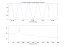
\includegraphics[width=120mm, height=70mm]{\HOME/figures/FTaperiodic}
}
\caption{{\small (top) The last four periods of a 220 Hz sine wave sampled
over the interval 0 to 0.743 seconds.  Since the wave can only
complete 163.47 cycles over this time interval, a concatenation of the
waveform (employed by the FFT and depicted by the dashed continuation
at $t=0.743$) introduces spurious frequency components into the signal.}}
\label{fig:FTaperiodic}
\end{figure}

Contrast the foregoing with what happens when the number of
observations in our sample set allows for an integral number
of periods.  This is easily accomplished when we are free to choose
all experimental parameters.  Suppose given are the sample rate, $SR =
44100$, and the number of observations $N=32768$, and suppose also that
we merely require the wave closely approximate the given frequency 
$f = 220$ Hz.  Then let   
\[
\tilde{f} = (SR/N)\lfloor (N/SR)f\rfloor \approx 219.37
\] 
The second factor, resulting from the ``floor'' operator $\lfloor \cdot
\rfloor$, represents the largest integer no greater than the number of
periods (163.47) completed by a 220 Hz wave during a sample time of
$N/SR$ seconds. 
As shown in Figure~\ref{fig:FTperiodic}, a concatenation of the
waveform -- depicted by the dashed continuation
at $t=0.743$ -- introduces no spurious frequency components.
\begin{figure}
\ifthenelse{\boolean{nofigures}}{}{
%             \pdfimage
%             width 88 mm 
%             height 60 mm
%%             width 13 cm
%%             height 10 cm
%             {\HOME/figures/FTperiodic.png}
\centering  
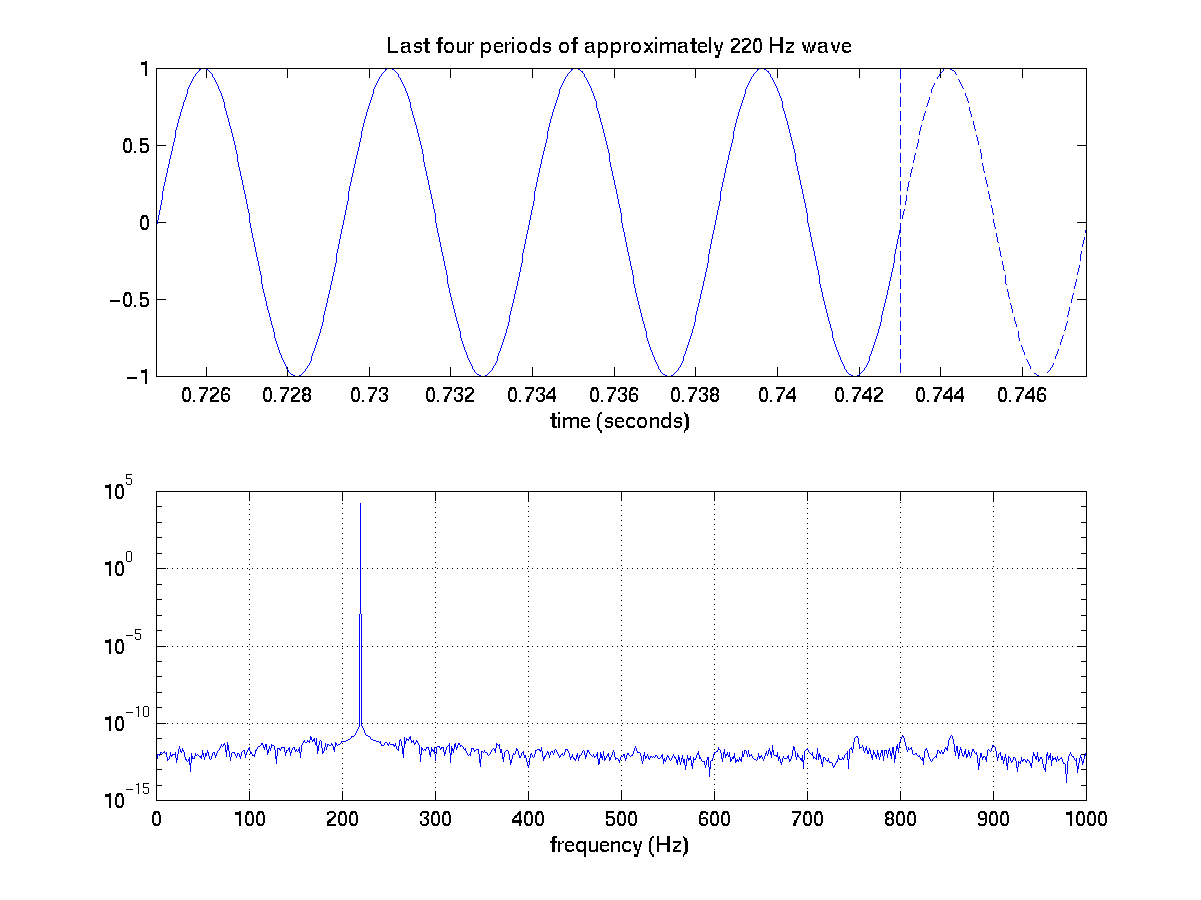
\includegraphics[width=120mm, height=70mm]{\HOME/figures/FTperiodic}
}
\caption{{\small (top) The last four periods of a 219.37 Hz sine wave sampled
over the interval 0 to 0.743 seconds.  Since the wave completes
exactly 163 cycles over this time interval, a concatenation of the
waveform (employed by the FFT and depicted by the dashed continuation
at $t=0.743$) introduces no spurious frequency components.}}
\label{fig:FTperiodic}
\end{figure}

From a practical point of view, it is natural to question the
utility of a method that depends on our ability to specify the
frequencies of the signals under study.
Instead, suppose we accept the signal frequencies as given and simply
adjust the number of samples used in the FFT to match the periods of
the existing frequencies.  Unfortunately, this is also impractical
when analyzing real sounds.  For, choosing this length
requires knowing the frequencies of the partials, and finding these
frequencies is precisely the FFT's raison d'\^{e}tre.

The problem -- exposed in Figure~\ref{fig:FTaperiodic} -- occurs because
the (empirical) ends of the signal don't line up; abrupt changes in
the waveform cause the spectrum to smear.  One way to force the ends
to line up is to preprocess the data so that it dies away to zero at
both ends.  Then, no matter what the underlying periodicity, there
will be no abrupt changes in the wave shape.

One popular approach is the \emph{Hamming} 
window\footnote{Named after Richard Hamming, this is a single cycle of
a scaled and shifted cosine wave.  The formula is $h(t) = 0.54 - 0.46
\cos(2\pi t/(N-1))$ for $0 \leq t < N$.  The Matlab code implementing
this technique is given in the appendix at section~\ref{sec:Sinewave}}.
The effect of the window on a 20 Hz wave is shown in
Figure~\ref{fig:hamming}.  The result of applying the window to a 220
Hz wave and then taking an $N$-point fast Fourier transform is
shown in Figure~\ref{fig:FThamming}. 
\begin{figure}
  \ifthenelse{\boolean{nofigures}}{}{
  \centering  
  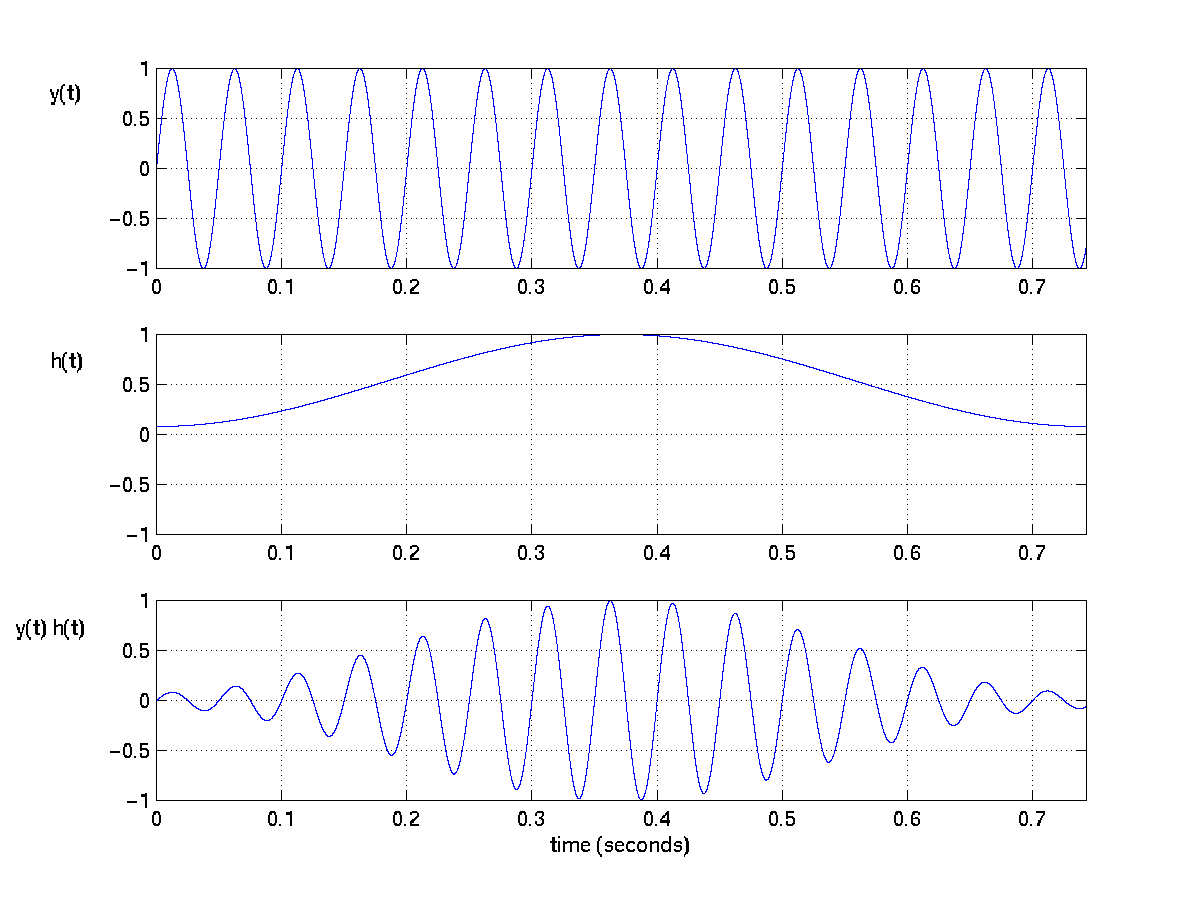
\includegraphics[width=120mm, height=70mm]{\HOME/figures/hamming}
  }
  \caption{{\small A 20 Hz sine wave (top) and a Hamming window (middle) are
  multiplied to produce the attenuated sine wave (bottom).}}
  \label{fig:hamming}
%\end{figure}
%
%\begin{figure}
  \ifthenelse{\boolean{nofigures}}{}{
  \centering  
  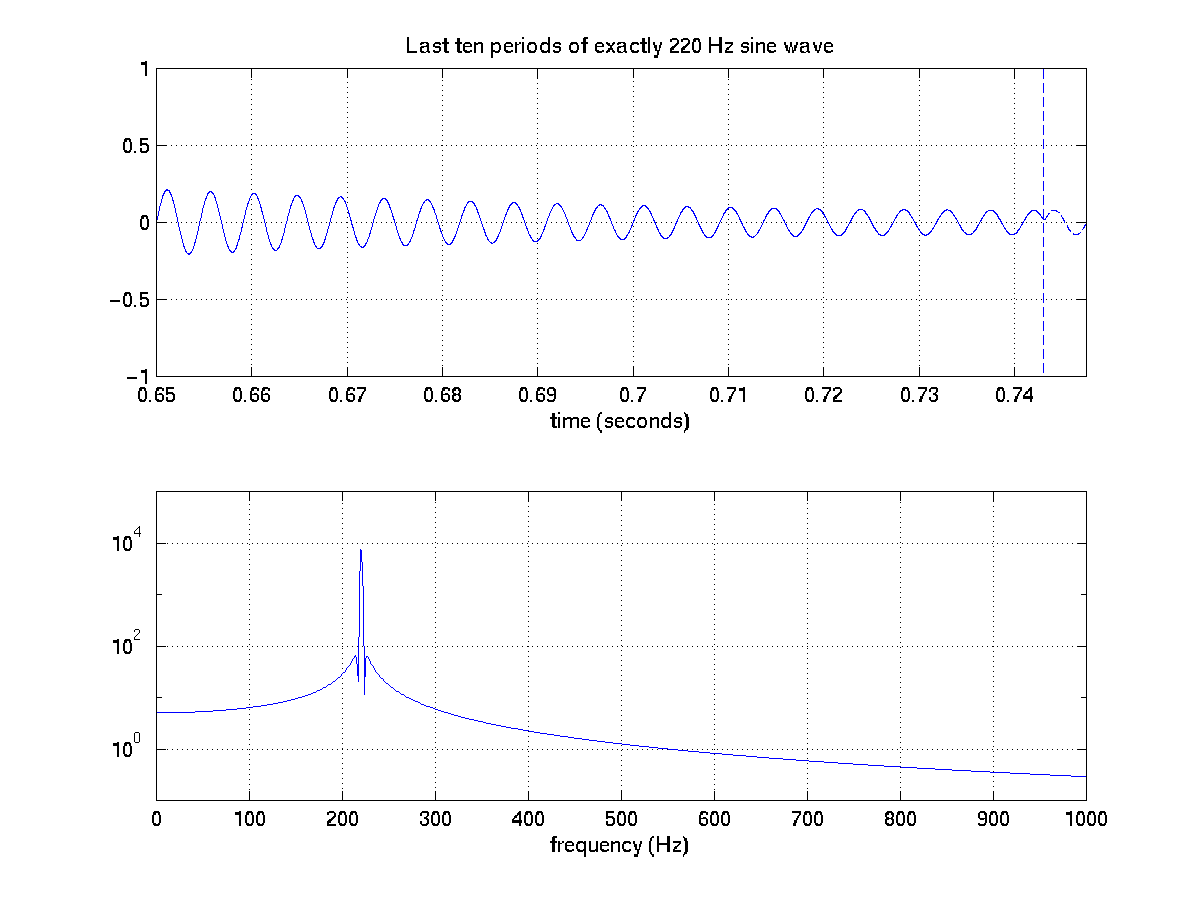
\includegraphics[width=120mm, height=70mm]{\HOME/figures/FThamming}
  }
  \caption{{\small (top) The last 10 periods of a 220 Hz windowed sine wave
  sampled over the interval 0 to 0.743 seconds.  Although the wave does
  not complete an integral number of periods over this time interval, a
  concatenation of the  waveform introduces less error than before
  because the wave is attenuated significantly at the point of
  aperiodicity ($t=0.743$).}}
  \label{fig:FThamming}
\end{figure}

The second cause of error when estimating the spectrum of a signal
concerns time versus frequency resolution.  The FFT measures the
frequency content of a signal on a given time interval, of length
$\Delta t$, over which we assume that the signal is approximately
stationary.  For real world signals, such as music, the approximation
gets worse as $\Delta t$ increases.  That is, the time intervals over
which we assume a constant frequency content must be small.
Precision in determining \emph{when} various frequencies
occur is the result of good or high \emph{time resolution}.

On the other hand, as the time resolution increases, the \emph{frequency
resolution} decreases.  This trade-off, a result of the well-known
\emph{uncertainty principle}, is illustrated by the following
scenario.  Assume a sample rate of $SR = 44100$ observations per second,
and a $4096$-point \emph{analysis window} (the interval over which to
compute the FFT).  This implies that each window examines $\Delta t =
N/SR \approx 0.093$ seconds of the signal.  In this case, the FFT measures
the frequency content of the signal by providing an $N$-element
vector of magnitudes indicating strength of spectral components at
(roughly) the frequencies {10.8 Hz, 21.5 Hz, \ldots, 44100 Hz}. The
general term in this sequence of frequencies is 
\[ 
k\times \frac{SR}{N} = k \times \frac{44100}{4096} 
		\approx k \times 10.77\text{ Hz,}
		\qquad  k\in\{1,2,\ldots, N\}
\] 
As shown by the top graph in Figure~\ref{fig:FFTbincomp}, the
frequency resolution is poor. 

Compare this to the same analysis at a lower time resolution, say
$\Delta t \approx 0.372$, obtained by setting $N= 16384$. This
provides the much clearer picture of the frequency content in the
bottom graph of Figure~\ref{fig:FFTbincomp}.  Still, the FFT only
indicates magnitudes at frequencies that are integer multiples of
$SR/N \approx 2.69$.  The presence in the signal of any frequency
components that \emph{are not} multiples of 2.69 (e.g.~220) is indicated by an
interpolation of the magnitudes at neighboring points (e.g.~218.0 and
220.7) which \emph{are} multiples of 2.69.
\begin{figure}
  \ifthenelse{\boolean{nofigures}}{}{
    \centering  
    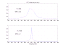
\includegraphics[width=120mm, height=70mm]{\HOME/figures/FFTbincomp}
  }
  \caption{{\small (top) The FFT of a 220 Hz windowed sine wave sampled over the
  interval 0 to 0.093 seconds. (bottom) The FFT of a 220 Hz windowed
  sine wave sampled over the interval 0 to  0.372 seconds.}  }
  \label{fig:FFTbincomp}
  %\end{figure}
  
  %\begin{figure}
  \ifthenelse{\boolean{nofigures}}{}{
    \centering  
    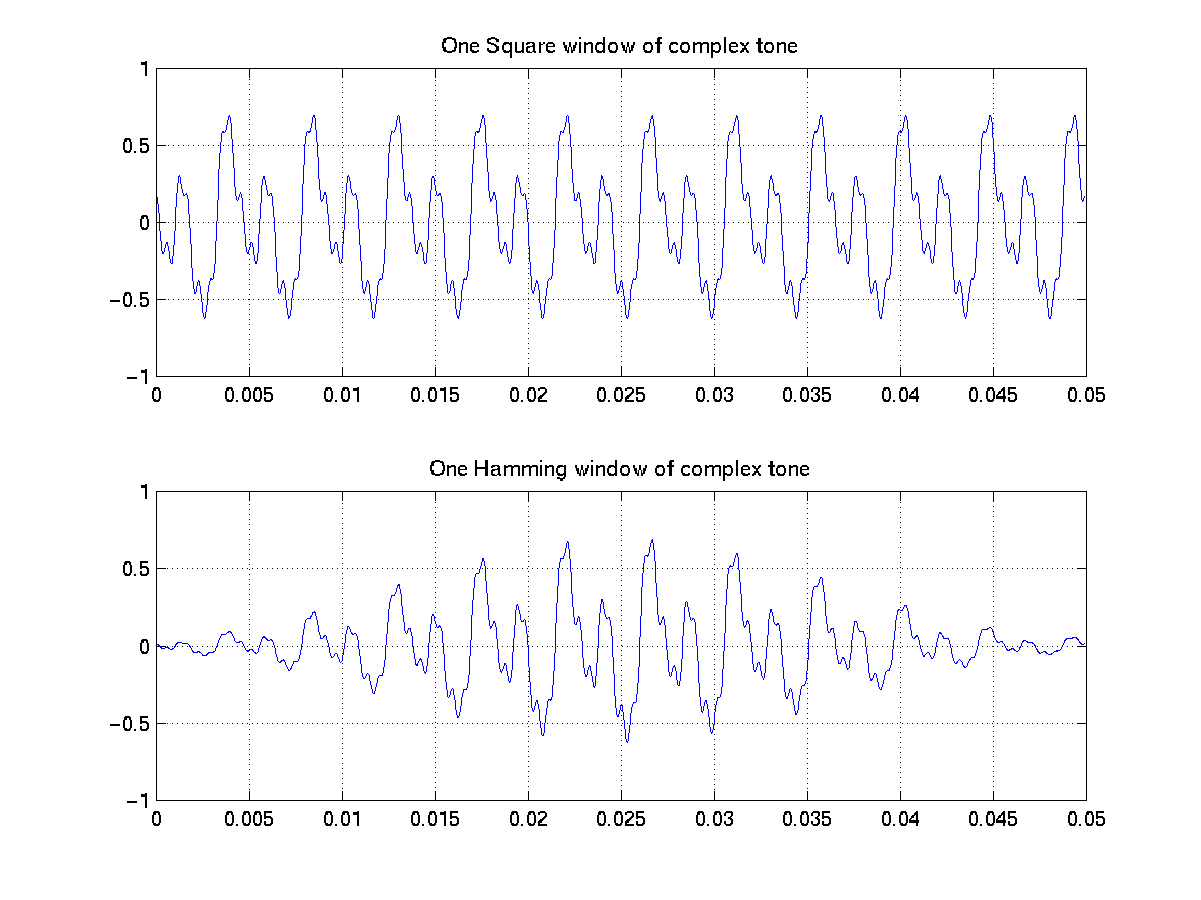
\includegraphics[width=120mm, height=70mm]{\HOME/figures/CompTone2200}
  }
  \caption{{\small A complex tone with frequencies 220, 440, 880, 1760 Hz and
  amplitudes .3, .4, .1, .1 (resp.) in a square window (top) and Hamming
  window (bottom) each of length 0.05 seconds.} }
  \label{fig:CompTone2200}
\end{figure}
  
\begin{figure}
  \ifthenelse{\boolean{nofigures}}{}{
    \centering  
    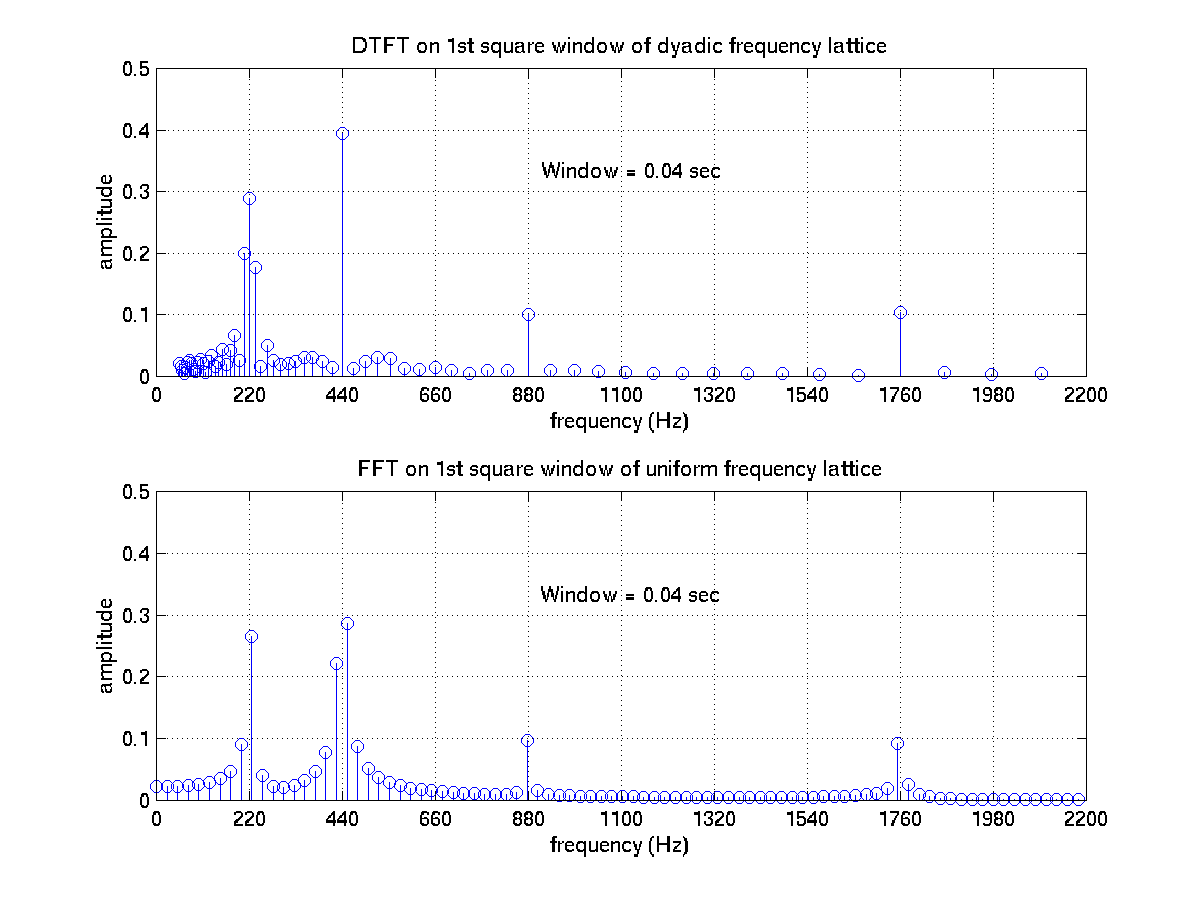
\includegraphics[width=120mm, height=70mm]{\HOME/figures/DTFTvFFTSq1760}
  }
  \caption{{\small The DTFT (top) and FFT (bottom) of a complex tone with
  frequencies 220, 440, 880, 1760 Hz and amplitudes .3, .4, .1, .1,
  (resp.) in a square window of length 0.04 seconds.}}
  \label{fig:DTFTvFFTSq1760}
  %\end{figure}
  
  %\begin{figure}
  \ifthenelse{\boolean{nofigures}}{}{
    \centering  
    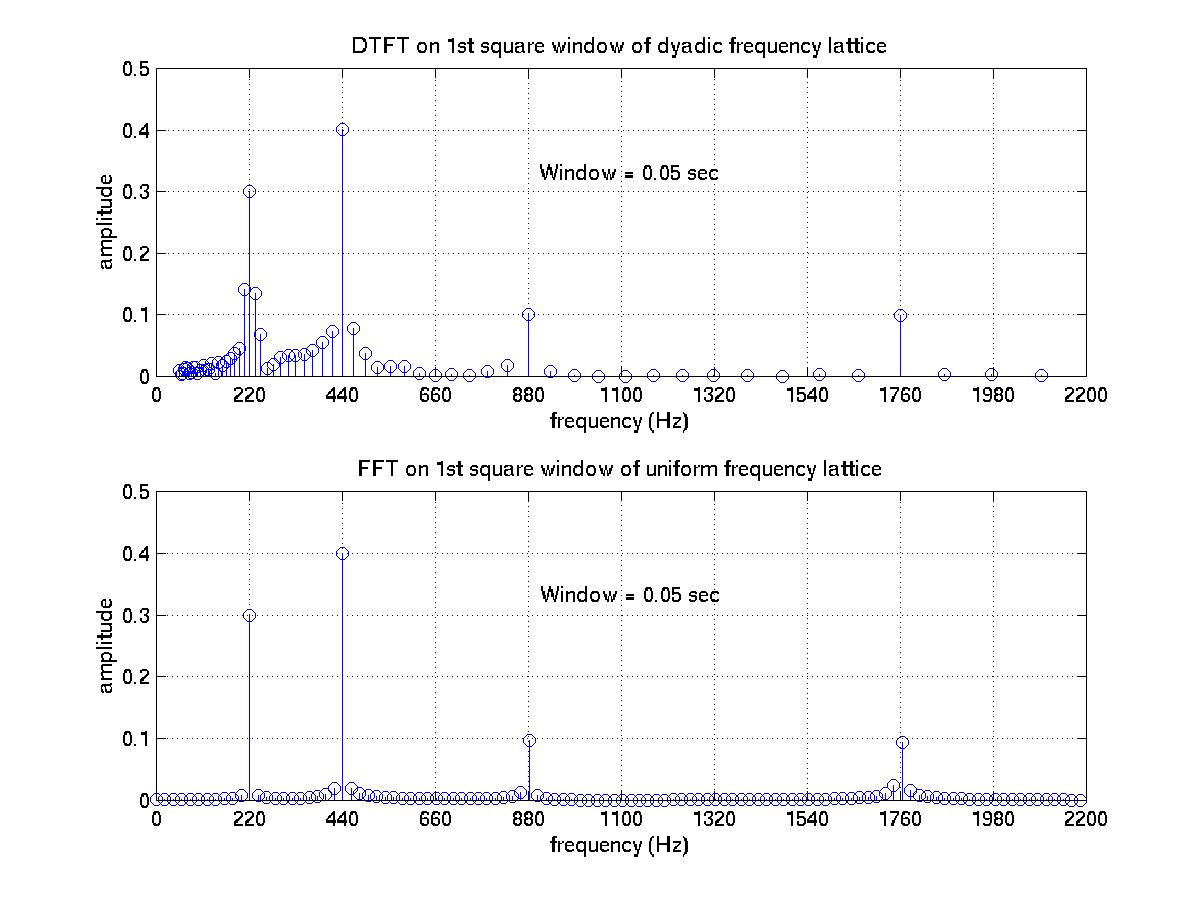
\includegraphics[width=120mm, height=70mm]{\HOME/figures/DTFTvFFTSq2200}
  }
  \caption{{\small The DTFT (top) and FFT (bottom) of a complex tone with
  frequencies 220, 440, 880, 1760 Hz and amplitudes .3, .4, .1, .1
  (resp.) in a square window of length 0.05 seconds.}}
  \label{fig:DTFTvFFTSq2200}
\end{figure}
%\begin{figure}
%             \pdfimage
%             width 13 cm
%%%             height 10 cm
%             {\HOME/figures/SpecDTFTHam1760.png}
%\caption{{\small The DTFT on a dyadic frequency lattice of a complex tone with
%frequencies 440, 880, 1320, 1760, 2200 Hz and amplitudes that start at .3, .4, .1, .1, .08,
%(resp.), decaying exponentially.}}
%\label{fig:SpecDTFTHam1760}
%
%             \pdfimage
%             width 13 cm
%%%             height 10 cm
%             {\HOME/figures/SpecFFTHam1760.png}
%\caption{{\small The FFT of a complex tone with frequencies 440, 880,
%1320, 1760, 2200 Hz and amplitudes that start at .3, .4, .1, .1, .08,
%(resp.), decaying exponentially.}}
%\label{fig:SpecFFTHam1760}
%\end{figure}
\begin{figure}
  \ifthenelse{\boolean{nofigures}}{}{
    \centering  
    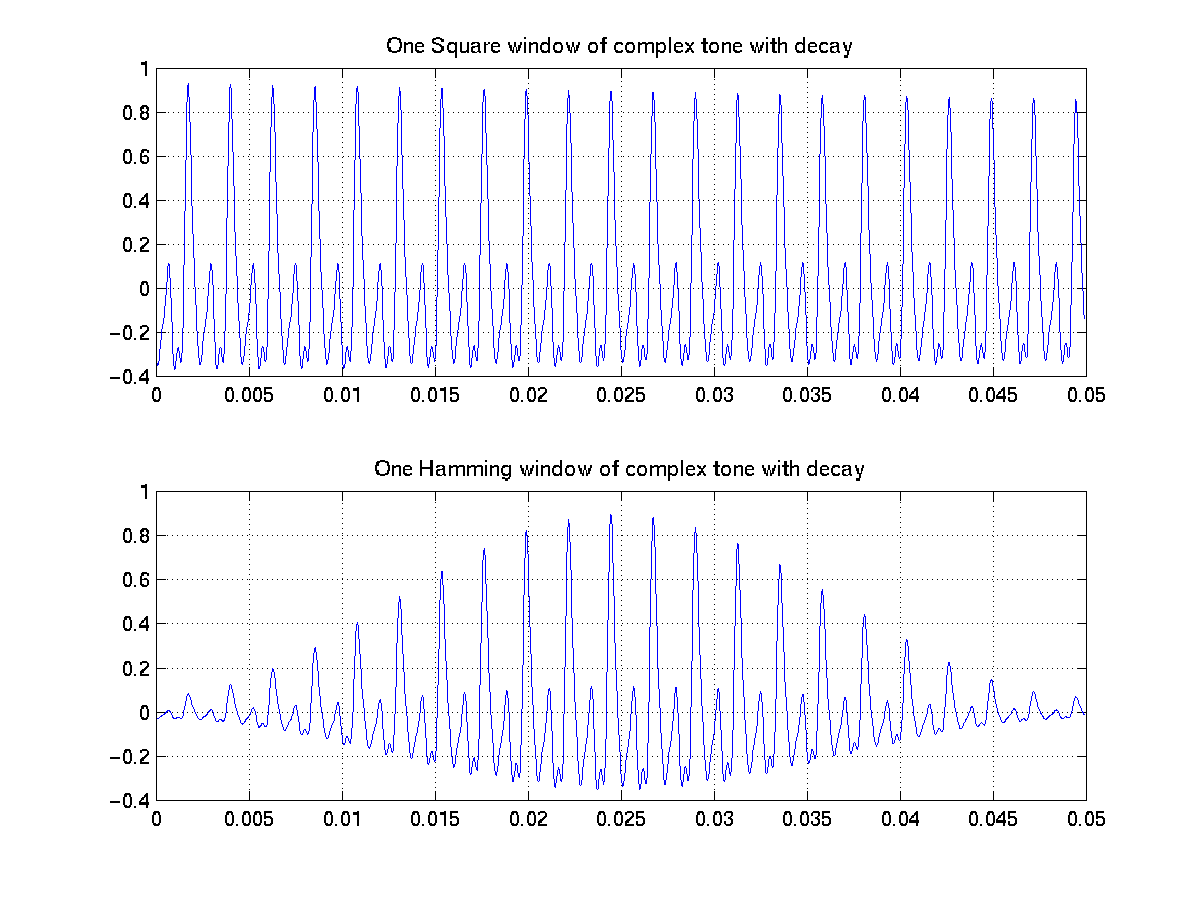
\includegraphics[width=120mm, height=70mm]{\HOME/figures/ComplexTone2200}
  }
  \caption{{\small A complex tone with frequencies 440, 880, 1320,
  1760, 2200 Hz and amplitudes that start at .3, .4, .1, .1, .08,
  (resp.), decaying exponentially. (top) a square window and (bottom) a
  Hamming window each of length 0.05 seconds.} }
  \label{fig:ComplexTone2200}
  %\end{figure}
  
  %\begin{figure}
  \ifthenelse{\boolean{nofigures}}{}{
    \centering  
    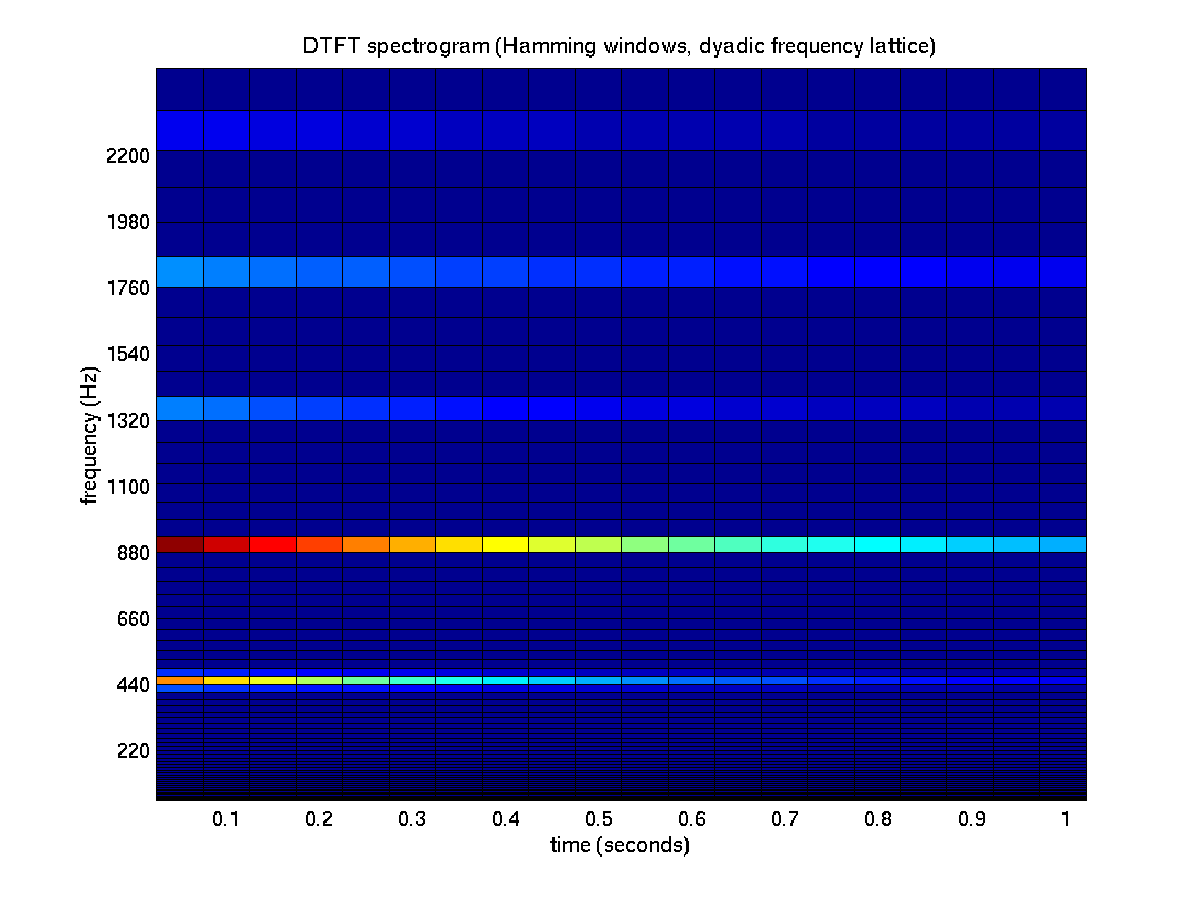
\includegraphics[width=120mm, height=70mm]{\HOME/figures/SpecDTFTHam2200}
  }
  \caption{{\small The DTFT of a complex tone with frequencies 440, 880, 1320,
  1760, 2200 Hz and amplitudes that start at .3, .4, .1, .1, .08,
  (resp.), decaying exponentially.  The time dimension is divided into
  0.05 second Hamming windows.  Amplitudes are computed along the
  frequency axis at the points $55 \cdot 2^{k/12}$ where $k=0, 1,
  \ldots, 96$.} }
  \label{fig:SpecDTFTHam2200}
\end{figure}
  
\begin{figure}
  \ifthenelse{\boolean{nofigures}}{}{
    \centering  
    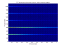
\includegraphics[width=120mm, height=70mm]{\HOME/figures/SpecFFTHam2200}
  }
  \caption{{\small The FFT of a complex tone with frequencies 440, 880,
  1320, 1760, 2200 Hz and amplitudes that start at .3, .4, .1, .1, .08,
  (resp.), decaying exponentially.  The time dimension is divided into
  0.05 second Hamming windows.  Amplitudes are computed along the
  frequency axis at 2200 evenly spaced frequencies.}}
  \label{fig:SpecFFTHam2200}
\end{figure}
% (end: insert file: SpectralEstimation.tex)

% (begin: insert file DissonanceEstimation.tex)
\subsection{Fourier Based Dissonance Estimation}
\label{sec:FourierDissonance}
Consider modeling the signal $f$ as the sum of partials,
\[
f(t) = \sum_j p_j(t)
\]
with $p_j(t) = a_j(t)\cos\phi_j(t)$ and 
$\phi_j(t)= \omega_jt+\phi_j$.
Measured in Hertz, the instantaneous frequencies of the partials are
$f_j  = \phi'_j(t)/2\pi$.
A measure of the sensory dissonance between two pure sinusoids, $p_j$
and $p_k$, can be based on the empirical research of Plomp and
Levelt~\cite{Plomp:1965} discussed earlier.  

At time $t_0$, assume that the values $f_j = \phi'_j(t_0)/2\pi$ and
$f_k = \phi'_k(t_0)/2\pi$ are known.  Then we define an
\emph{instantaneous dissonance} measure between the two partials as
follows: 
%\begin{eqnarray*}D[a_j(t_0)\cos\phi_j(t),a_k(t)\cos\phi_k(t)]\\
\[
D[p_j,p_k](t_0)= a_j(t_0)a_k(t_0)d(f_j,f_k)
\]
%\end{eqnarray*}
For the metric $d(\cdot,\cdot)$ we employ the parameterization of the
Plomp-Levelt curves given by Sethares~\cite{Sethares:1997},
\begin{equation}
\label{eqn:diss}
d(f_j,f_k) = e^{-b_1x} - e^{-b_2x}
\end{equation} 
where $x(t) = |f_j - f_k|/\min\{f_j,f_k\}$.  The constants
$b_1$ and $b_2$ determine the rate at which the dissonance curve rises
and falls. %~\cite{Plomp:1965},
Sethares performed a gradient minimization of the squared error between
the function~(\ref{eqn:diss}) and the averaged Plomp and
Levelt data.  This values $b_1 = 3.5$ and $b_2=5.57$ produce the best
fit. 

Next, we define the \emph{instantaneous dissonance}
of the signal $f$ at time $t_0$ as the sum
\begin{equation}
\label{eqn:instDiss}
Df(t_0)= \frac{1}{2}\sum_{j,k}a_j(t_0)a_k(t_0)d(f_j,f_k)
\end{equation}

Of course, in general we cannot assume that the amplitudes and
instantaneous frequencies are known.  However, we can approximate
these data by assuming them constant over the time support
%Heisenberg boxes 
of each windowed Fourier atom $g_{s,u,\xi}$.  This assumption permits a 
measure of dissonance at each window including time $t_0$ for which
$(t_0,\xi(t_0))$ is a ridge point.  We take this as our estimate of
the instantaneous dissonance over the time window containing $t_0$.
More precisely, let $W_{t_0}=[t_{-},t_{+}]$ be the window containing
$t_0$.  At each ridge 
point $(t_0,\xi_j(t_0))$, with $t_0\in W_{t_0}$, we estimate 
\[
\tilde{f}_j = \xi_j(t_0)/2\pi, \qquad %\text{ and }\quad
\tilde{a}_j = \frac{2|Sf(t_0,\xi_j(t_0)|}{\sqrt{s}|\hat{g}(0)|}
\]
We take as our estimated sensory dissonance over the interval
$t \in W_{t_0}$ 
\begin{equation}
\label{eqn:estDiss}
\tilde{D}f(t)= 
\frac{1}{2}\sum_{j,k}\tilde{a}_j\tilde{a}_k d(\tilde{f}_j,\tilde{f}_k)
\end{equation}

\begin{figure}
  \ifthenelse{\boolean{nofigures}}{}{
    \centering  
    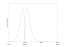
\includegraphics[width=120mm, height=70mm]{\HOME/figures/analyticDiss}
  }
  \caption{The exact dissonance curve computed with \emph{a priori}
  knowledge of the amplitudes and frequencies.  The horizontal axis
  delimits time, though the tick marks indicate the frequency of the
  linear tone.} 
  \label{fig:analyticDiss}
%\end{figure}

%\begin{figure}
  \ifthenelse{\boolean{nofigures}}{}{
    \centering  
    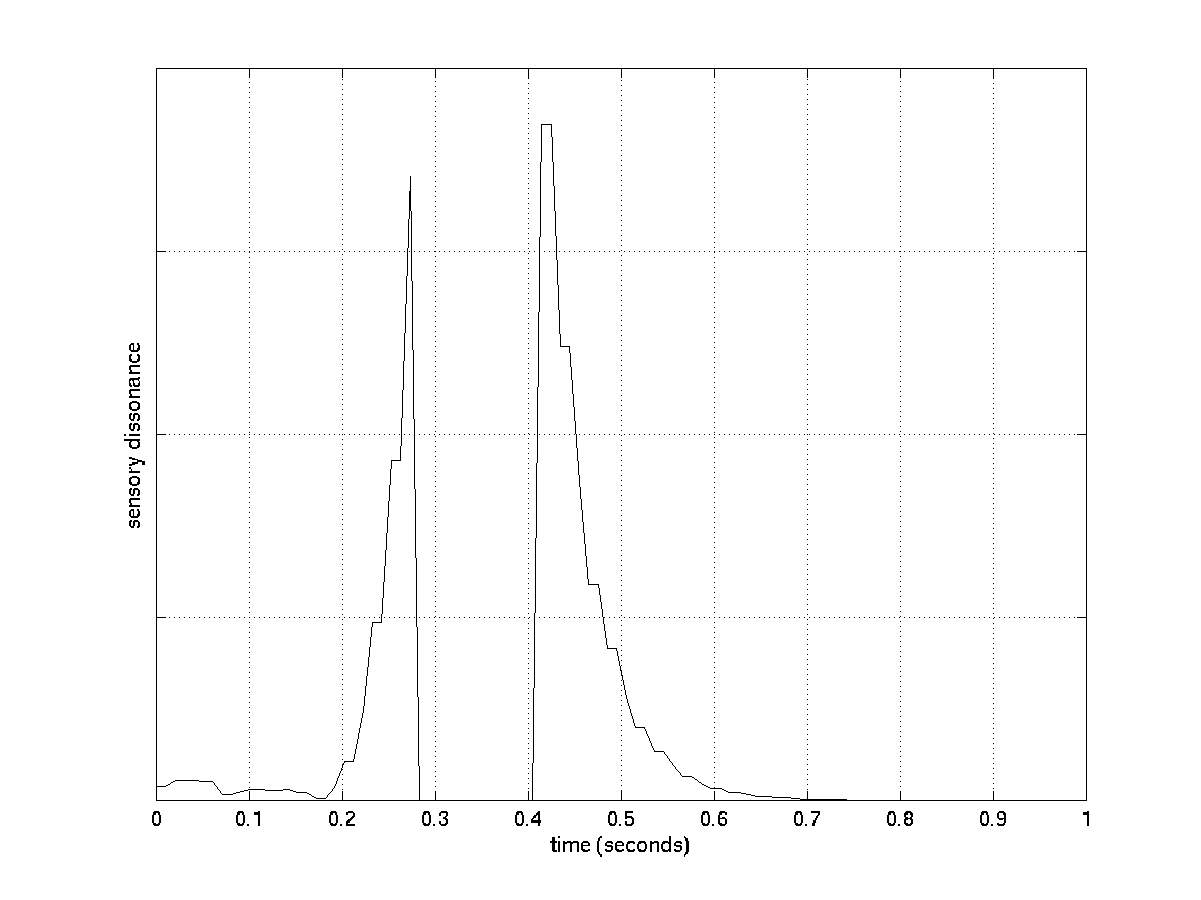
\includegraphics[width=120mm, height=70mm]{\HOME/figures/empiricalDiss}
  }
  \caption{The estimated dissonance curve computed with 
  ridge point estimates of amplitudes and frequencies.}
  \label{fig:empiricalDiss}
\end{figure}

Figure~\ref{fig:analyticDiss} shows the instantaneous dissonance of
the signal~(\ref{eqn:purelin440}) as $t$ varies over $[0,1]$.  It is
computed using~(\ref{eqn:instDiss}).  Figure~\ref{fig:empiricalDiss}
shows the estimated dissonance of the same signal.  It is computed
by taking amplitude and frequency estimates from the ridges in
Figure~\ref{fig:ridges} and plugging them into~(\ref{eqn:estDiss}).
As we can see, the windowed Fourier atoms do not provide a high enough
frequency resolution to provide a reliable dissonance measure on the
interval $t\in[.3,.4]$.  This corresponds to a frequency interval
for the linear chirp of about $[418, 484]$ Hz.  
For a musical
%If this were a musical 
signal, this implies that only frequency intervals of more than 2
semitones are distinguishable.  One might argue that, for a method to
be useful for musical applications, it must be able to discriminate 
between two components that are one semitone apart.  
%This provides a
%clear objective for future work, and a criteria by which such work
%may be judged. 
% (end: insert file DissonanceEstimation.tex)

\subsection{Matching Pursuit}
\label{sec:Practical-MP}
This section describes how we implement the atomic decomposition
of a signal using the matching pursuit algorithm described in
section~\ref{sec:MP}.  

The Matlab program {\tt MZMP.m}, appearing in section~\ref{sec:MZMP},
computes the optimal gabor atoms for representing a given signal.  
The primary sub-routines it calls are {\tt gaborMZ.m} and {\tt IP.m},
which listed in sections~\ref{sec:gaborMZ} and~\ref{sec:IP},
respectively.  The {\tt gaborMZ} sub-routine computes individual
gabor atoms given a set of parameters.  (Section~\ref{sec:MP}
describes the parameters that define a gabor atom.)  The {\tt IP}
sub-routine computes the inner product of two gabor atoms from
their given parameters without actually constructing the atoms.

\subsection{Energy Separation}
\label{sec:Practical-energy-separation}
This section describes the implementation of the energy separation
technique described in section~\ref{sec:energy-separation}.

The Matlab program {\tt DEnergy.m} appears in
section~\ref{sec:DEnergy}, and computes the \emph{signal energy}
and \emph{interference energy} of a given signal.  (The italicized
terms are defined in section~\ref{sec:energy-separation}.)  The first
step in this process is a call to the {\tt MZMP} routine, which
computes the matching pursuit decomposition of the signal. The output
of {\tt MZMP} are the parameters of a collection of gabor atoms
which optimally represent the given signal. Next, the Wigner and
cross-Wigner transforms of these optimal atoms are computed by calling
the sub-routines {\tt WVTrans\_AF.m} and {\tt WVTrans\_AFC.m},
respectively.  Finally, the {\tt DEnergy} routine (optionally)
produces a time-frequency display of the signal energy and
interference energies.

\subsection{Energy Based Dissonance Estimation}
\label{sec:EnergyDissonance}


\pagebreak

\appendix
\begin{center}
{\bf APPENDIX}
\end{center}
% -*- mode: LaTeX; tex-main-file: "../notes.tex"; -*-
%\subsection{Basic Analysis}
\section{Math Background and Notes}
\ifthenelse{\boolean{nofootnotes}}{\subsection{Inner Product Spaces}}
{\subsection{Inner Product Spaces\protect\footnotemark}
\footnotetext{Mertins~\cite{Mertins:1999}, (p.~4).}}
The signal spaces we consider are the spaces $\Ltwo(a,b)$ and
$\ltwo(n_1,n_2)$.  On these we can define an {\it inner product} which 
assigns a complex number to two signals $x(t)$ and $y(t)$, or  
$x(n)$ and $y(n)$, respectively.  Denoted 
$\langle x,y\rangle$,
the inner product must satisfy the following axioms:
\begin{enumerate}
\item $\langle x,y\rangle = \langle y,x\rangle^*$
\item $\langle \alpha x + \beta y, z\rangle =
  \alpha\langle x,z\rangle +\beta\langle y,z\rangle$ 
\item $\langle x,x\rangle \geq 0, \qquad \langle x,x\rangle = 0 \Leftrightarrow x = \mathbf{0}$
\end{enumerate}
Here, $\alpha, \beta \in \C$ are scalars, and $\mathbf{0}$ is the null vector.

Some examples of inner products that we employ in the present work are
\begin{alignat*}{2}
%\label{eqn:RInnerProd}
\langle x,y\rangle &= \integral x(t)y^*(t)\,dt, && \qquad x,y\in \LtwoR \\
\langle x,y\rangle &= \int_{a}^{b} x(t)y^*(t)\,dt, && \qquad x,y\in \Ltwo(a,b) \\
%\label{eqn:ZInnerProd}
\langle x,y\rangle &= \sum_{n=-\infty}^{\infty} x(n)y^*(n), && \qquad x,y\in \ltwoR \\
\langle x,y\rangle &= \sum_{n=n_1}^{n_2} x(n)y^*(n), && \qquad x,y\in\ltwo(n_1,n_2)
\end{alignat*}
Each of the foregoing definitions of $\langle x,y\rangle$ corresponds to an
associated vector space, appearing on the right, of which $x$ and $y$ are members.  Therefore,
the meaning of $\langle x,y\rangle$ will often be clear from the space on which it is used.

%\subsection{Operator Theory}
\ifthenelse{\boolean{nofootnotes}}{\subsection{Linear Operators}}
{\subsection{Linear Operators\protect\footnotemark}
\footnotetext{For more details consult Teolis~\cite{Teolis:1998} or
  Rudin~\cite{Rudin:1991}} }
This section reviews some of the operator theory cited in this
paper.

The Banach space of bounded linear operators that map the Hilbert
space %$\mathcal{H}_1$ 
$\Hone$ to the Hilbert space $\Htwo$ is denoted $\Banachonetwo$.
%$\mathcal{B}(\mathcal{H}_1,\mathcal{H}_2)$
The \emph{norm} of an element $\T \in \Banachonetwo$ is
\[ 
\|\T \| = \sup_{x\in\Hone} \frac{\|\T[x]\|_{\Htwo}}{\|x\|_{\Hone}} < \infty
\]
Two classes of operators specifically worthy of mention are
the self-adjoint operators and the orthogonal projection operators.
\begin{define}{\bf Self-Adjoint. } (\cite{Teolis:1998} Fact 2.2)
If $\T \in \Banach$ is \emph{self-adjoint} then
\[ 
\|\T \| = \sup_{f\in\mathcal{H}} \frac{|\langle f,\T[f] \rangle|}{\|f\|^2}.
\]
\end{define}
\begin{define}{\bf Orthogonal Projection. } (\cite{Teolis:1998} Fact
2.3)
Let $\mathcal{X}$ be a subspace of the Hilbert space $\mathcal{H}$ and
let $\P_{\mathcal{X}}: \mathcal{H} \mapsto \mathcal{X}$ denote the
\emph{orthogonal projection operator} onto $\mathcal{X}$.  The operator
$\P_{\mathcal{X}}\in \Banach$ is an orthogonal projection 
onto $\mathcal{X}$ if and only if $\P^2_{\mathcal{X}} = \P_{\mathcal{X}}$
and $\P_{\mathcal{X}}$ is self-adjoint.
\end{define}

Following the exposition in Teolis~\cite{Teolis:1998}, we now
state some important properties of linear operators.
Let $\Hone$ and $\Htwo$ be arbitrary Hilbert spaces with norms 
$\|\cdot\|_{\Hone}$ and $\|\cdot\|_{\Htwo}$ and inner products
$\langle \cdot,\cdot\rangle_{\Hone}$ and
$\langle \cdot,\cdot\rangle_{\Htwo},$ respectively.
Let $\T$ be an operator that maps a function in $\Hone$ to a function
in $\Htwo$; that is, $\T: \Hone \mapsto \Htwo$.
\begin{enumerate}
\item The \emph{range} of $\T$ is 
$\T (\Hone) \equiv \{\T[f]: f\in \Hone\}$.
\item The \emph{kernel} (or \emph{null space}) of $\T$ is 
$\Null(\T ) \equiv \{f \in \Hone: \T[f] = 0\}$.
\item $\T $ is \emph{injective} (or \emph{one-to-one}) when $\T[f] = \T g$ if and
only if $f = g$.  If $\T $ is a linear operator then $\T $ is injective if
and only if $\Null(\T ) = \{0\}$.
\item $\T $ is \emph{surjective} or \emph{onto} if $\T (\Hone) = \Htwo$.
\item $\T $ is \emph{bijective} if it is both injective and surjective.
\item $\T $ has an \emph{inverse} $\T ^{-1}: \Htwo \mapsto \Hone$ if $\T $ is
bijective.  In this case the inverse of $\T $ is defined as $\T ^{-1}g =
f,$ where $f$ is such that $\T[f]=g$.
\item $\T $ is \emph{continuous} if $x_n \mapsto x$ implies $\T[x]_n \mapsto x$.
A linear operator is bounded if and only if it is continuous.
\item The \emph{adjoint} of $\T $ is the unique operator 
$\T ^*:\Htwo \mapsto \Hone$ for which
$\langle \T[f],g\rangle_{\Htwo} = \langle f,\T ^*g\rangle_{\Hone}$ holds for all
$f\in \Hone$ and $g \in \Htwo$.  $\T $ is \emph{self-adjoint} if
$\T ^*=\T $.
\item $\T \in \Banachonetwo$ is a \emph{compact} operator if, for all
sequences $\{f_n: \|f_n\| = 1\} \subseteq \Hone$, the sequence
$\{\T[f]_n\}$ has a converging subsequence in $\Htwo$.
\item $\T $ is a \emph{topological isomorphism} if $\T $ is bijective,
$\T \in \Banachonetwo$, and $\T ^{-1} \in \Banachtwoone$.  Thus, both $\T $
and $\T ^{-1}$ are continuous linear operators.
\item $\T $ is an \emph{isometry} if for all $f \in \Hone$,
$\|\T[f]\|_{\Htwo} = \|f\|_{\Hone}$.
\item $\T $ is a \emph{unitary} map if it is linear, bijective, and an
isometry.  If $\T $ is unitary then $\T ^{-1} = \T ^*$.
\end{enumerate}

\ifthenelse{\boolean{nofootnotes}}{\subsection{Integral Transforms}}
{\subsection{Integral Transforms\protect\footnotemark}
\footnotetext{Mertins~\cite{Mertins:1999}, (p.~22).}}
The integral transform is one of the most important tools in signal theory.
The best known example is the Fourier transform, which we describe in
section~\ref{sec:Fourier}, but there are many other transforms of interest.

The basic idea of an integral representation is to describe a signal $x(t)$
via its density $\hat{x}(t)$ with respect to an arbitrary {\it kernel}, denoted
$\phi(t,s)$.  This is done as follows:
\begin{equation}
\label{eqn:kernel}
x(t) = \int_S \hat{x}(s) \phi(t,s) \,ds, \hspace{1cm} t\in T
\end{equation}
A {\it reciprocal kernel}, $\theta(s,t)$, may be found such that the density
$\hat{x}(s)$ can be calculated in the form
\begin{equation}
\label{eqn:reciprocal}
\hat{x}(s) = \int_T \hat{x}(t) \theta(s,t) \,dt, \hspace{1cm} s\in S
\end{equation}
Substituting (\ref{eqn:reciprocal}) into (\ref{eqn:kernel}) yields,
\begin{equation}
\label{eqn:recipkern}
x(t) =  \int_T x(\tau) \int_S \theta(s,\tau) \phi(t,s) \,ds\,d\tau
\end{equation}
The {\it Dirac impulse} $\delta(t)$ satisfies such an integral equation:
\begin{equation}
\label{eqn:dirac}
x(t) =  \integral \delta(t-\tau) x(\tau) \,d\tau, \hspace{1cm} x\in \LoneR
\end{equation}
From equation (\ref{eqn:recipkern}) and definition (\ref{eqn:dirac}), we arrive
at the following:
\[
  0 = \int_T x(\tau) \left(\int_S \theta(s,\tau)\phi(t,s)\,ds -
      \delta(t-\tau)\right) \,d\tau 
\]
which holds for all $x$ if and only if 
\[
  \int_S \theta(s,\tau)\phi(t,s)\,ds = \delta(t-\tau)
\]
If, instead, we substitute equation (\ref{eqn:kernel}) into
(\ref{eqn:reciprocal}) and proceed as above, {\it mutatis mutandis}, 
we arrive at 
\[
\int_T \phi(t,\xi)\theta(s,t)\,dt = \delta(s-\xi)
\]
\begin{define}{\bf Self-Reciprocal Kernels. } A special category is that of
\emph{self-reciprocal kernels}.  They correspond to orthonormal bases and
satisfy $\phi(t,s) = \theta^*(s,t)$, so that
\begin{eqnarray}
\label{eqn:selfreciprocal}
\int_S \theta(t,s)\theta^*(s,\tau)\,ds&=& \int_S \theta(s,t)\phi(\tau,s)\,ds\\
&=&\delta(t-\tau) \nonumber
\end{eqnarray}
\end{define}
Transforms that contain a self-reciprocal kernel are also called {\it unitary}
because they yield $\|\hat{x}\| = \|x\|$, by Parseval's relation, which we
cover in the following section.

\ifthenelse{\boolean{nofootnotes}}{\subsection{Parseval's Relation}}
{\subsection{Parseval's Relation\protect\footnotemark}
\footnotetext{Mertins~\cite{Mertins:1999}, (p.~25).}}
\label{sec:Parseval}
Let the signals $x(t)$ and $y(t)$ be square integrable, $x,y \in \Ltwo(T)$.
For the densities, let
\begin{eqnarray}
\hat{x}(s) &=& \int_T x(t) \theta(s,t) \,dt\nonumber \\
\label{eqn:densities}
\hat{y}(s) &=& \int_T y(t) \theta(s,t) \,dt
\end{eqnarray}
where $\theta(s,t)$ is a self-reciprocal kernel satisfying
(\ref{eqn:selfreciprocal}). 
Now consider inner products
\begin{eqnarray}
  \langle x,y\rangle &= &\int_T x(t)y^*(t)\,dt\nonumber \\
\label{eqn:innerproducts} 
  \langle \hat{x},\hat{y}\rangle &= & \int_S \hat{x}(s)\hat{y}^*(s)\,ds 
\end{eqnarray}
Substituting the densities (\ref{eqn:densities}) into the the inner product
(\ref{eqn:innerproducts}) yields
\[ 
  \langle \hat{x},\hat{y}\rangle =
  \int_S \int_T \int_T x(\tau)\theta(s,\tau) y^*(t) \theta^*(s,t) \,d\tau \,dt \,ds
\] 
By self-reciprocity, the foregoing becomes
\begin{eqnarray*}
  \langle \hat{x},\hat{y}\rangle &=&
  \int_T x(\tau)\int_T y^*(t) \delta(t-\tau) \,dt \,d\tau\\
&=&  \int_T x(\tau) y^*(\tau) \,d\tau
\end{eqnarray*}
This proves {\it Parseval's relation}
\[ 
  \langle \hat{x},\hat{y}\rangle =   \langle x,y\rangle 
\]
For $y(t)=x(t)$, Parseval's relation shows that self-reciprocal
kernels are unitary, as claimed in the preceding section:
\[ 
  \langle \hat{x},\hat{x}\rangle = \langle x,x\rangle 
  \hspace{7mm} \Rightarrow \hspace{7mm} \|\hat{x}\|=\|x\|
\]

%\subsection{Spectral Analysis}
\subsection{Fourier Transforms}
\label{sec:Fourier}
\begin{define}{\bf Continuous-Time Fourier Transform. } 
% \footnote{For a more detailed development see
% Mallat~\cite{Mallat:1998} or Teolis~\cite{Teolis:1998}.} 
The mapping $\mathcal{F}: \LtwoR \mapsto \LtwoR$, defined for
$x\in \LoneR \subset \LtwoR$ by
\begin{equation}
\label{eqn:FT}
\mathcal{F}[x](\omega) = \hat{x}(\omega) = \integral x(t) e^{-i2\pi\omega t}\,dt
\end{equation}
is called the \emph{continuous-time Fourier transform}.  Throughout
the paper, we reserve the special notation $X(\omega)$ and $Y(\omega)$
for the Fourier transforms of $x(t)$ and $y(t)$, respectively.

For $x \in \LtwoR \setminus \LoneR$, the continuous-time \FT\ is defined
\[
X(\omega) = 
\lim_{n\rightarrow \infty}\int_{-n}^n x(t) e^{-i2\pi\omega t}\, dt
\]
In the latter case, convergence of the limit to $X$ is in the
$\Ltwo$-sense.
\end{define}
The quantity $X(\omega)$ measures how much oscillation at
frequency $\omega$ there is in the signal $x(t)$.
If $x \in \LoneR,$ the integral in (\ref{eqn:FT}) does converge and 
\[|X(\omega)| \leq \integral |x(t)|dt \]
Therefore $X$ is bounded and it is a continuous function of $\omega.$
If $X$ is also integrable, the inverse Fourier transform is 
\begin{equation}
\label{eqn:InvFT}
x(t) = %\frac{1}{2\pi}
\integral X(\omega) e^{i2\pi\omega t} \,d\omega
\end{equation}
which gives the decomposition of the signal $x(t)$ as a weighted sum of sinusoidals
$\exp\{i2\pi\omega t\}$ with weights (amplitudes) given by $X(\omega)$.
If we define the inner product of the functions $x$ and $y$ to be
\[
\langle x,y \rangle = \integral x(t) y^*(t)\,dt
\]
then $X(\omega) = \langle x,e^{i2\pi\omega} \rangle$.  This operation can
be viewed as the projection of $x$ onto $e^{i2\pi\omega}$ since 
%\[\langle f - X e^{i2\pi\omega}, e^{i2\pi\omega} \rangle = 0\]
%that is, 
the function $x - X e^{i2\pi\omega}$ is orthogonal to
$e^{i2\pi\omega}$. 

To summarize, the inverse Fourier transform (\ref{eqn:InvFT})
represents the reconstruction of $x(t)$ as the sum of its projections
onto the basis functions $\{e^{i2\pi\omega t}\}$.  Thus, it is simply a
more general version of the decomposition appearing in
equation~(\ref{eqn:sumcos}): 
\[
x(t) = \sum_{k=1}^K a_k \cos(\omega_k t + p_k)
\]

The sinusoidal functions $\{e^{i2\pi\omega t}\}$ are useful as building
blocks for signals, especially those that do not change quickly over time.
However, it is possible to find other \emph{atomic} functions that
provide a better 
%\marginpar{\em We must consider the criteria
%by which we judge one basis to be better than another.}
basis on which to project signals that have more
dramatic stuctural variations.  
The goal of an atomic decomposition is to provide a recipe for
constructing a given function $x\in \mathcal{H}$ out of a set of atomic
functions $\{\phi_n\}$.  Analysis is restricted to recipes of the form
\begin{equation}
\label{eqn:lincomb}
x(t) = \sum c_n \phi_n(t) 
\end{equation}
where $\{c_n\}$ is a countable sequence in $\ltwoR$ and the atoms
satisfy some fundamental properties.  For instance, the basic
requirement is that the atoms span the space $\mathcal{H}$ -- that is,
every element $x \in \mathcal{H}$ can be written as a linear
combination of the atoms, as in~(\ref{eqn:lincomb}).

\begin{define}{\bf Discrete-Time Fourier Transform. } Let $x(n)$ be a
discretized version of the analog signal considered above.  If $x(n)$
is absolutely summable, that is $\sum|x(n)| < \infty$, then its
\emph{discrete-time Fourier transform} is given by 
\begin{equation}
\label{eqn:DTFT}
\mathcal{F}[x_n](\omega) = X(\omega) = \sum_{n=-\infty}^{\infty}x(n) e^{-i2\pi\omega n}
\end{equation}
The \emph{inverse discrete-time Fourier transform} of $X(\omega)$ is
given by 
\begin{equation}
\label{eqn:InvDTFT}
x(n) = %\frac{1}{2\pi}
\integral X(\omega) e^{i2\pi\omega n} \,d\omega
\end{equation}
\end{define}
The operator $\mathcal{F}$ transforms a discrete signal $x(n)$ into a
complex-valued continuous function $X(\omega)$ of the real
variable $\omega$, which is a digital frequency measured in Hertz.

If $x(n)$ is of finite duration, then Matlab can be used to compute
$X(\omega)$ numerically at any freuqency $\omega$.  The approach
is to implement~(\ref{eqn:DTFT}) directly.  If, in addition, we wish to
evaluate $X(\omega)$ at the set of frequencies
$\{\omega_1,\ldots,\omega_M\}$, then~(\ref{eqn:DTFT}) can be
implemented as a simple matrix-vector multiplication.  For example,
suppose $x(n)$ has $N$ samples between $n_1 \leq n \leq n_2$.  
% and that we want to evaluate $X(\omega)$
Then~(\ref{eqn:DTFT}) can be written as
\begin{equation}
\label{eqn:nDTFT}
X(\omega_k) = 
\sum_{\ell=1}^{N}x(n_{\ell}) e^{-i2\pi\omega_k n_{\ell}}, \; k = 1, \ldots, M
\end{equation}
When $\{x(n_{\ell})\}$ and $\{X(n_{\ell})\}$ are arranged as
column vectors $\mathbf{x}$ and $\mathbf{X}$, respectively, 
equation~\ref{eqn:nDTFT} is equivalent to 
\[\mathbf{X} = \W \mathbf{x}\]
where $\W$ is an $M \times N$ matrix given by 
\[
\W = 
\left\{e^{-i2\pi\omega_k n_{\ell}} : n_1 \leq n \leq n_2, 1 \leq k \leq M \right\}
\]
If we arrange $\{\omega_k\}$ and $\{n_{\ell}\}$ as \emph{row} vectors
$\mathbf{w}$ and $\mathbf{n}$ repsectively, then 
\[
\W =
\left[\exp{(-i2\pi\mathbf{w}^t \mathbf{n})}\right] \in \C^{M\times N}
\]
We will make use of this direct computation of the discrete-time
Fourier transform in the experiments of section~\ref{sec:practical}.

% (begin: inserted from file energydensity.tex)
%\protect\footnotemark}
%\footnotetext{Mallat~\cite{Mallat:1998} (p.110)}
\begin{define}{\bf Unitarity. }  
The Parseval relation (\ref{sec:Parseval}) shows that the Fourier transform is
an isometry of $\LtwoR$.  Thus, the inner product of two signals remains the
same, no matter if we represent it in the time or frequency domain:
$\langle X,Y\rangle = \langle x,y\rangle$.  
It follows that the temporal and spectral energy densities,
respectively $|x(t)|^2$ and $|X(\omega)|^2$, %/2\pi  
satisfy the energy conservation equations
\begin{align*}
\|x\|^2 &= \integral |x(t)|^2\,dt  \\
%        &=\langle x,x\rangle =\langle X,X \rangle 
%                           \qquad \text{ (Parseval's) }\\ 
        &=\integral |X(\omega)|^2\,d\omega = \|X\|^2
\end{align*}
\end{define}

\emph{Moyal's formula}~\cite{Moyal:1949} proves that the \WT\ is also
  unitary, an thus yields similar energy conservation properties.
\begin{theorem}[Moyal\footnote{See also~\cite{Mallat:1998}, p.110, for
  a proof.}]
For any $x$ and $y$ in $\LtwoR$
\begin{eqnarray}
\left|\langle x,y\rangle\right|^2 &=& 
\left|\integral x(t)y^*(t)dt\right|^2 \nonumber \\
&=&%\frac{1}{2\pi}
\iint \W_x(t,\nu)\W_y(t,\nu) \,dt \,d\nu
\label{eqn:Moyal}
\end{eqnarray}
\end{theorem}
% (end: inserted from file energydensity.tex)

\ifthenelse{\boolean{nofootnotes}}{\subsection{Cohen's Class}}
{\subsection{Cohen's Class\protect\footnotemark}
\footnotetext{Mallat~\cite{Mallat:1998}, (p.114).}}
Above we claimed that time-frequency energy densities,
%$\P_x(u,\omega)$, 
such as the spectrogram and scalogram, are time-frequency averagings
of the \WT. To see this, reconsider the family $\{\phi_{\gamma}\}$  
of time-frequency atoms from section~\ref{sec:atomic}, where for any
$(u,\omega)$ there exists a unique atom $\phi_{\gamma(u,\omega)}$
centered in time-frequency at $(u,\omega)$. The corresponding linear
time-frequency transform of $x$ is 
\[
\T[x](u,\omega) =\langle x,\phi_{\gamma(u,\omega)} \rangle
\]
%       &&=\integral x(t)\phi^*_{\gamma}(t)\,dt \nonumber \\
The resulting time-frequency energy density is
\begin{eqnarray*}
E_{T[x]}(u,\omega)&
  =&\left|\langle x,\phi_{\gamma(u,\omega)}\rangle\right|^2 \\
 &=& \left|\integral x(t) \phi^*_{\gamma(u,\omega)}(t)\,dt\right|^2
\end{eqnarray*}
Moyal's formula~(\ref{eqn:Moyal}) proves that this energy density is a
time-frequency averaging of the \WV\ transform:
\[
E_{T[x]}(u,\omega)= %\frac{1}{2\pi}
\iint \W_x(t,\nu)\W_{\phi_{\gamma(u,\omega)}}(t,\nu)\,dt\,d\nu
\]
The smoothing kernel is the \WV\ transform of the atoms
\[\theta(u,t,\omega,\nu) =
%\frac{1}{2\pi}
\W_{\phi_{\gamma(u,\omega)}}(t,\nu)\]
The loss of time-frequency resolution depends on the spread of the
transform $\W_{\phi_{\gamma(u,\omega)}}(t,\nu)$ in the neighborhood of
$(u,\omega)$. To summarize, positive time-frequency transforms totally
remove the interference terms, but produce a loss of information.


% The following now appears in math.tex
% \input{\HOME/theory/Fourier}
% -*- mode: LaTeX; tex-main-file: "../notes.tex"; -*-
\section{Perception of Complex Tones}
This section contains notes on the perception of complex tones.  In
particular, we focus on two concepts that are related to 
%have connections to 
the ideas in the paper, but which are not described therein, as they
are not immediately relevant.  This material is included here because
it might be useful in future work. 
%The last part of this section presents some notes on the music we use
%in the experiments of section~\ref{sec:practical}. 
% (begin: insert file fusion.tex)
\subsection{Tonal Fission and Fusion} 
In this section are some notes on tonal fusion.  First are excerpts
from Sethares~\cite{Sethares:1997} (p. 25, 26), and then some brief notes
from Hartmann~\cite{Hartmann:1998}. 

Almost all musical sounds consist of a great many partials, whether they are
harmonically related or not.  Using techniques such as selective damping and
the selective excitation models, it is possible to learn to ``hear out'' these
partials, to directly perceive the spectrum of the sound.  This kind of
listening is called \emph{analytic} listening, as compared to \emph{holistic}
listening in which the partials fuse together into one perceptual entity.

Consider the closing chord of a string quartet.  At one extreme, is the fully
analytic listener that ``hears out'' a large number of individual partials.
At the other extreme is the fully holistic listener who hears the chord as one
grand ``tone,'' all four instruments fusing into a single rich and complex
sonic texture.  Typical listening lies somewhere in between: the partials of
each instrument fuse, but the instruments remain individually perceptible,
each with its own pitch, loudness, vibrato, etc.  What physical cluesmake this
remarkable feat of perception possible?

When listeners are presented with clusters of partials and asked how many
distinct voices, notes, etc. they hear, various features of the presentation
reliably encourage tonal fusion.  Some of these features are whether the
partials:
\begin{enumerate}
\item begin at the same time (attack synchrony),
\item have similar envelopes (amplitudes change similarly over time),
\item are harmonically related, or
\item have the same vibrato rate.
\end{enumerate}
Almost any common feature of a subgroup of partials helps them to be perceived
together. 

Hartmann~\cite{Hartmann:1998} (p. 134) states that the most important mediator of
perceptual segregation and integration is the onset time of the tones, which
he calls \emph{onset synchronicity} (cf. attack syncrony of Sethares).  If two
sets of partials have different onset times, then the auditory system
segregates them as different entities.  

A study by Rasch (1978) indicates that 30ms advanced onset leads to 40dB
increase in level perception and allows the listener to segregate while
remaining unaware of the 30ms asynchrony.  However, research by Risset,
Matthews (1969) and Beauchamp (1975) shows that the harmonics of high
frequencies lag those of low frequencies by greater than 30ms\footnote{A
  diagram of this phenomena is in the comp book at (00.07.10).}
% (end: insert file fusion.tex)

% (begin: insert file dominance.tex)
\ifthenelse{\boolean{nofootnotes}}{\subsection{Spectral Dominance}}
{\subsection{Spectral Dominance\protect\footnotemark }
\footnotetext{This topic is also discussed in Hartmann
\cite{Hartmann:1998}.}}
A periodic complex tone has a pitch that is equal to, or slightly less
than, the frequency of the fundamental. 
Assuming the various overtones of a complex tone fuse together to
create an overall pitch, just how these overtones are combined is a
question of great interest.  In particular, if a complex tone is
composed of pure sinusoidal partials, each having a given frequency
and amplitude, which of these partials will be more pronounced and make a
greater contribution to the determination of the fundamental (low) pitch of
the complex tone?  A promising experimental approach is to mistune one
or more partials and study the effect on the synthesized low pitch.
Experiments by Ritsma (1967) and Moore, Glasberg, and Peters (1985)
led to the conclusion that the partials that are most important in
determining the low pitch are those that are resolved by the auditory
periphery.  Retsma concluded that for fundamental frequencies between
100 and 400 Hz, partials three, four, and five are dominant.  Terhardt
(1974) proposed a dominant frequency range centered on 700 Hz, instead
of particular harmonic numbers.  Moore {\it et al}.~concluded that the
dominant partials were among the first six, but individual differences
prevented them from being more specific.

The observed importance of the resolved harmonics supports the idea
that pitch perception takes place at high levels where excitations
from different peripheral channels are recombined.  Pattern matching
or template fitting models focus on this idea.  The model studied by
Goldstein (1973) derives the low pitch from a pattern match to the
frequencies of the higher partials.
% (end: insert file dominance.tex)

\section{Sound Examples}
This section presents some notes on the music, used in the
experiments of section~\ref{sec:practical}.

\subsection{\emph{Metamorphosis} (1988), by Philip
Glass\protect\footnotemark} 
\footnotetext{This brief presentation is based on that of Kerman and
Tomlinson~\cite{Kerman:2000}} 
\begin{define}{\bf Philip Glass (b.~1937) }
%studied at the University of Chicago and with
%Persichetti, Bergsma, and N. Boulanger and
may be the most wide-ranging of the minimalist composers.  He plays
keyboards in a crossover group, the Philip Glass Players, which has
appeared in concert halls and art museums, at rock clubs and jazz
festivals.  He has written music for some remarkable art films; he
collaborates with the innovative multimedia artist Robert Wilson.  The
easy-to-play piano piece that this paper examines makes a much quieter
statement than the famous Glass pieces such as his operas and ensemble
numbers written for his group.  Nevertheless, \emph{Metamorphosis} is
typical of the composer's work in its constructive principles and
overall effect.

\emph{Metamorphsis} consists of five very similar movements of
approximately the same length.  In \emph{Metamorphosis 1}, three brief
elements alternate, without transitions of any kind to link them.  The
first element, {\bf a}, announces four chords in a slow dotted rhythm;
the second, {\bf b}, introduces gentle motion, oscillating quietly
between two notes of a simple chord.  This music is utterly
uneventful, except that the bass comes in halfway through the
four-measure span.  The third element, {\bf c}, is a fragment of
melody -- repetitive, plaintive, built over harmonies similar to those
of {\bf a}, and with a fluid accompaniment continuing from {\bf b}.
The dynamic never rises above mezzo forte.  

This simple plan for \emph{Metamorphosis 1} can be represented
\newcommand{\Aa}{\mathbf{a}}
\newcommand{\Bb}{\mathbf{b}}
\newcommand{\Cc}{\mathbf{c}}
\[ ||: \Aa \; \Bb \; \Aa \; \Bb \; \Cc \; \Bb \; \Cc \; \Bb \; \Cc \; \Bb :|| \; \Aa' \; \Aa' \; \Aa' \; \Bb \; \Bb \; \Bb 
\mbox{ (repeated three times)}\]
where $\Aa'$ is an extension of the four-chord series to five -- a
telling change in these inert surroundings.  Notice that although the
ending of the chord series features rich and rather melancholy chords,
the way the three elements are juxtaposed somehow leaches all the
expressivity out of them.  One waits fascinated for that inevitable
bass entry in b.
\end{define}
\section{A Note on Numerical Precision}
\subsection{Numerical Support of Gabor Atoms}
Here we remark on some practical considerations which we may want to
account for in future (more numerically precise) constructions of the
Gabor dictionary. 

Suppose we begin with a general gaussian function
\[
g(t) = e^{-\alpha t^2}, \qquad t \in \R,\; \alpha > 0
\]
Then we translate $g$ in time by $p$, scale it by $s$, and
modulate it by $f$ Hz, yielding 
\[
g_\gamma(t) = Kg\left(\frac{t-p}{s}\right)e^{i2\pi ft} 
= Ke^{-\alpha \left(\frac{t-p}{s}\right)^2}e^{i2\pi ft} 
\]
where $\gamma = (p,s,f)$ denotes the paramter vector and $K$ is chosen
so that $\|g_\gamma\|=1$.

Clearly $g > 0$ for all $t$, and $g(t)\rightarrow 0$ as $t\rightarrow
\pm \infty$.  Thus, the \emph{theoretical support} of %both $g$ and
$g_\gamma$ is the entire real line (minus the zeros resulting from
the frequency modulation). However, for practical applications in
which we are restricted to finite precision arithmetic, it is
important to consider the \emph{numerical support} of $g_\gamma$,
which is necessarily a finite subset of $\R$.  In other words, we must
consider for what values of $t$ is it the case that $g_\gamma(t) \geq
\epsilon_m$. Here $\epsilon_m$ is the \emph{machine epsilon}, defined 
as the smallest positive number attainable by the computer.  For
example, on our Pentium II hardware, the Matlab function {\tt eps}
returns
\[
\epsilon_m \approx  2.22 \times 10^{-16}
\]
Clearly, when $t$ is such that $|g_\gamma(t)| < \epsilon_m$, the
computer perceives $g_\gamma(t)$ as no different from 0, and we must
assume that the function is not numerically supported on these values
of $t$.

Let us now find the numerical support of $g_\gamma$, for $p = 0$; that
is, for $\gamma = (0,s,f)$.
% (This can be generalized for $p>0$ with a
%simple time translation.)
\begin{eqnarray}
|g_\gamma(t)| \geq \epsilon_m 
&\Leftrightarrow& 
|K e^{-\alpha \left(\frac{t}{s}\right)^2}e^{i2\pi ft}| \geq
\epsilon_m \\ 
&\Leftrightarrow& 
K e^{-\alpha \left(\frac{t}{s}\right)^2} \geq \epsilon_m \\ 
&\Leftrightarrow& 
-\alpha \left(\frac{t}{s}\right)^2 
\geq \log\epsilon_m - \log K \nonumber\\ 
& \Leftrightarrow & \left(\frac{t}{s}\right)^2 \leq
\frac{\log K -\log\epsilon_m}{\alpha}\nonumber\\ 
\label{eqn:support}
& \Leftrightarrow & 
|t| \leq s\left(\frac{\log K -\log\epsilon_m}{\alpha}\right)^{1/2}
\end{eqnarray}
Since $\epsilon_m$ is a small positive number,
$\log K-\log\epsilon_m$ is positive.  Thus, the square root in
the last inequality of (\ref{eqn:support}) results in a positive real
number, and defines the numerical support of $g_\gamma$. 

It is convenient to choose $\alpha$ such that the numerical support of
$g_\gamma$ is $[-s/2,s/2]$.  
%$g$ is $[-1/2,1/2]$.  
%Then scaling by $s$ results in a scaled gaussian,
%$g_s(t) = g(t/s)$, with numerical support $[-s/2,s/2]$.  
However, such an $\alpha$ is difficult to acheive analytically because
the normalization constant $K$ depends on $\alpha$ and $s$.
So, we proceed by deriving $K$ and $\alpha$ analytically as far as
possible, and then we consider a numerical optimization 
that will yield Gabor atoms having the desired numerical support.

We seek $K$ such that $\|g_\gamma\| = 1$, where
\[
g_\gamma(t) = Ke^{-\alpha \left(\frac{t}{s}\right)^2}e^{i2\pi ft},
\qquad t \in \R,\; \alpha > 0
\]
and
%\begin{eqnarray*}\begin{align*}
\[
\|g_\gamma\|^2 = \integral g_\gamma(t)g_\gamma^*(t)\,dt
               = K^2\integral
        e^{-2\alpha\left(\frac{t}{s}\right)^2}\,dt\\ 
\]
%\end{eqnarray*}\end{align*}
%Recall that a gaussian density integrates to 1. For a density with
%variance $\sigma^2$, this means 
%\begin{equation}\label{eq:gaussint}
%\frac{1}{\sigma \sqrt{2\pi}} \integral e^{-t^2/2\sigma^2}\,dt = 1
%\end{equation}
%Using this fact, we derive the following
Such a $K$ is derived as follows:
\begin{align*}
1 = \|g_\gamma\|^2 &= K^2\integral
    e^{-2\alpha\left(\frac{t}{s}\right)^2}\,dt\\ 
\Leftrightarrow \quad K^{-2} &=
\integral e^{-2\alpha\left(\frac{t}{s}\right)^2}\,dt
%\end{align*}
%This holds if, and only if,
%\begin{eqnarray*}
\\
\Leftrightarrow \quad K^{-2}
&=\integral\exp\left\{-\frac{t^2}{2(s/2\sqrt{\alpha})^2}\right\}\,dt
\end{align*}
Letting $\sigma= \frac{s}{2\sqrt{\alpha}}$, the foregoing is
equivalent to 
\[%\begin{equation}\label{eq:K}
K^{-2} = %\sigma \sqrt{2\pi} \frac{1}{\sigma \sqrt{2\pi}}
\integral e^{\frac{-t^2}{2 \sigma^2}}\,dt\\
       = \sigma \sqrt{2\pi}
\]%\end{equation}
The final equality obtains from the fact that a gaussian density integrates to 1.
%Fact~(\ref{eq:gaussint}) 
%Finally, equation~(\ref{eq:K}) 
This shows that the value of $K$ resulting in atoms of unit
norm is  
\[
K=(\sigma \sqrt{2\pi})^{-1/2}=\left(\frac{2\alpha}{\pi s^2}\right)^{1/4}
\]
Inserting this expression into equation (\ref{eqn:support}), which
defines the numerical support, we have
\begin{equation}
\label{eq:alpha}
\frac{\log K -\log\epsilon_m}{\alpha} =\frac{1}{4}
\left(\frac{\log\alpha-2\log s - 4\log\epsilon_m+\log(2/\pi)}
           {\alpha}\right) 
\end{equation}
Recall from (\ref{eqn:support}) that we seek a value of $\alpha$ such
that the right hand side of equation~(\ref{eq:alpha}) is
equal to 1/4.  This occurs when 
\[
\alpha = \log \alpha -2\log s - 4\log \epsilon_m+\log(2/\pi)
\]
which is nonlinear in $\alpha$.  Therefore, for given values of $s$,
we select numerically optimal values of $\alpha$ by minimizing the
function 
\[
L_s(\alpha)=
|\alpha - \log\alpha + 2\log s + 4\log\epsilon_m-\log(2/\pi)|
\]
The Matlab routine {\tt fminbnd.m} accomplishes this effectively.  We
use it as follows:
\begin{verbatim}
>> fn = inline('abs(x-log(x)+4*log(eps)+2*log(P1)-log(2/pi))',1);
>> alpha = fminbnd(fn,1,200,optimset('Display','off'),S);
\end{verbatim}

%However, numerical
%experimetation shows that the $\log \alpha$ term is well approximated
%by a linear function of $r = \log_2 s$.  After some simulation,
%we find that the following definition of $\alpha$ yields suitable
%numerical supports for the scaled gaussians $g_\gamma(t)$,
%\[
%\alpha =  5 - 0.01 r - 2\log s - 4\log \epsilon_m + \log(2/\pi),
%\quad \text{ where } s = 2^r.
%\]





%%% (erroneous) characteristic function derivation %%%
%
%&=& K^2 \integral e^{i4\pi ft} e^{-2 \alpha \left(\frac{t}{s}\right)^2}\,dt\\
%&=& K^2 \integral 
%    e^{i4\pi ft} \exp\left\{\frac{-t}{2 (s/2\sqrt{\alpha})^2}\right\}\,dt
%\end{eqnarray*}
%Now let $\sigma= \frac{s}{\sqrt{\alpha}}$, yielding
%\begin{eqnarray*}
%\|g_\gamma\|^2 
%&=& K^2 \sigma \sqrt{2\pi} \frac{1}{\sigma \sqrt{2\pi}}
%\integral e^{i4\pi ft} \exp\left\{\frac{-t^2}{2 \sigma^2}\right\}\,dt\\
%&=& K^2 \sigma \sqrt{2\pi} \phi_X(f)\\
%&=& K^2 \sigma \sqrt{2\pi} 
%    \exp\left\{\frac{-\sigma^2(4\pi f)^2}{2}\right\}
%\end{eqnarray*}
%The last equality holds because the integral that we have labelled
%$\phi_X(f)$ is the characteristic function of $X$, a normal random
%variable with mean 0 and variance $\sigma^2$.
%

\pagebreak
% -*- mode: LaTeX; tex-main-file: "../notes.tex"; -*-
\section{Description of Matlab Routines}
%%%% New Matlab Code begins here:
First briefly state what each routine does, then we will give a more
detailed description of the main routines below.
The file {\tt beats.m} constructs and returns an example signal.
For example, 
\begin{verbatim}
   >> signal = beats(K); 
\end{verbatim}
constructs a signal of length $N = 2^{K+1}$.  Specifying signal
length with the argument K -- representing one less than the integer
power of 2 -- has certain advantages that become clear
later. Briefly, no matter what value is given for K, the signal
length will always be a power of 2, which is useful for certain
algorithms. Also, knowing the relation $N=2^{K+1}$, and having the
pair $N,K$ at our disposal, facilitates handling the dictionary of 
Gabor atoms; we use atoms with scales of size $2^j$ where $j$ ranges
from 1 to $K$. 

The file {\tt Dictionary.m} contains code for computing and storing
the parameters of all atoms in a Gabor dictionary, as well as
storing the correlations of these atoms with the given signal. (If
we know the signal length in advance, it is possible to precompute
all the atoms and store them to disk.  However, depending on the speed
of our algorithms for computing atoms on the fly, this may not be
the most efficient approach, since it would require retrieval of atoms
from slow memory). 

Here is an example call to {\tt Dictionary}, with the analytic signal
specified in the row vector {\tt signal}:
\begin{verbatim}
>> [P,C]=Dictionary(signal,DEBUG,DISP);
\end{verbatim}

Now that we have a dictionary of Gabor atoms, and the correlations
of each atom with the signal, we can call the (Mallat/Zhang)
Matching Pursuit routine, {\tt MZMP}:
\begin{verbatim}
>> [MaxP, MaxC]=MZMP(signal,ITERS,TOL,P,C,DEBUG,DISP); % run MP on signal
\end{verbatim}
In the argument list appears {\tt ITERS}, the maximum number of
iterations, which is equivalent to the maximum number of atoms with
which to approximate the signal; {\tt TOL} is the error tolerance were
willing to accept; {\tt P} is the matrix of parameters for all the atoms
in the dictionary; {\tt C} is a vector of the signal-atom correlations,
for all the atoms in the dictionary.  The routine returns {\tt MaxP}
which is a matrix of parameters defining the atoms having the best
correlation to the signal (or its remainder at each step of the matching
pursuit), and {\tt MaxC}, which are those maximum correlation values.

Finally, the routine {\tt DEnergy.m} takes the results from {\tt MZMP}
and computes the Wigner energy and interferences. An example call of
this routine is:
\begin{verbatim}
>> [WVE, WVI]=DEnergy(signal,MaxP,MaxC,DEBUG,DISP);  % find WV
\end{verbatim}

\subsection{Energy Separation}\label{sec:DEnergy}
\begin{verbatim}
function [WVE,WVI,P_DEnergy,C_DEnergy] = DEnergy(sig,DEBUG,DISP,P,C);
\end{verbatim}
The {\tt DEnergy.m} function computes energy and interference by calling
the matching pursuit routine MZMP, and then the Wigner transform and
cross Wigner transform routines, WVTrans\_AF and WVTrans\_AFC. 
\begin{small}\begin{verbatim}
% Inputs
%   sig       1-dimensional signal of interest
%   DEBUG     (default 1) DEBUG=0 => do not print extra debugging info
%   DISP      (default 1) DISP=0 => do not display plot of results
%   P         optional input array of atom parameters from a prior run
%   C         optional input vector of atom correlations from a prior
%             run  
%
% Outputs
%   WVE       complex-valued matrix representing the sum of the
%             Wigner transforms of each atom in the collection of atoms
%             used to represent the signal. Rows correspond to
%             frequencies and columns corresponding to times.
%   WVI       Same as WVE except that *cross* Wigner transforms are
%             summed.
%   P_DEnergy optionally stored array of atom parameters
%   C_DEnergy optionally stored vector of atom correlations
%
% Usage
%  >> pause off; [WVE,WVI,P_DEnergy,C_DEnergy]=DEnergy;
%  >> [WVE,WVI] = DEnergy(sig,1,1,P_DEnergy,C_DEnergy);
%
% See also:  MZMP, gaborMZ, WVTrans_AF, WVTrans_AFC
%
% Author: William DeMeo <william.demeo@verizon.net>
% Date: 2001 July 20
% Copyright (c) 2001, William DeMeo

if nargin < 1, 
  disp('DEnergy: no signal input... proceding with synthetic signal demo.');
  K=8; N=pow2(K+1);       % signal length
  %%% synthetic signal params (signal should really be an input) %%%%
  f1 = .1; f2 = 2*f1; f3 = 3*f1; %f1 = 440/N; f2 = 2*f1; f3 = 3*f1;
  sig=atoms(N,[1,f1,pow2(K-2),.75; 1,f2,pow2(K-2),.25; ...
    pow2(K),f2,pow2(K-2),1; 3*pow2(K-1),f3,pow2(K-2),.5]);
else,  
  N=length(sig); K=nextpow2(N)-1; 
end;
if nargin < 2, DEBUG=1; end;
if nargin < 3, DISP=1; end;

% Matching Pursuit parameters
MAXITERS=20; 
TOLERANCE=0.05;

if nargin < 5,
  if(DEBUG),disp('DEnergy: computing new atoms with MZMP...');end;
  %%% CALL MATCHING PURSUIT FUNCTION %%%
  [P,C] = MZMP(sig,MAXITERS,TOLERANCE,DEBUG);
end;
% store a local copy of parameter/correlation book of atoms 
P_DEnergy = P; C_DEnergy = C;  % (and return it if requested)

% P is at most a size MAXITERSx4 array; C is at most 1xMAXITERS
M = size(P,1);     % M = number of atoms used in signal representation
WVE = zeros(N,N);
WVI = zeros(N,N);

if(DEBUG),disp('DEnergy: computing energy & interference...');end;
for n=1:M-1,
  [g1,Ks] = gaborMZ(K,P(n,1),P(n,2),P(n,3));
  WV = WVTrans_AF(g1,0);
  WVE = WVE + (abs(C(n))^2)*WV;
  for m=n+1:M,
    [g2,Ks] = gaborMZ(K,P(m,1),P(m,2),P(m,3));
    WV = WVTrans_AFC(g1,g2,0);
    WVI = WVI + 2*real(C(n)*conj(C(m))*WV);
  end;
  if(DEBUG),disp(sprintf('DEnergy: finished atom %d of %d',n,M));end;
end;

[g1,Ks] = gaborMZ(K,P(M,1),P(M,2),P(M,3));
WV = WVTrans_AF(g1,0);
WVE = WVE + (abs(C(M))^2)*WV;

if(DISP),
  figure(1);clf;
  absE = real(WVE);
  tfmax = max(max(absE));
  tfmin = min(min(absE));
  colormap(1-gray(256));
  image(linspace(0,1,N),linspace(0,1,N),256*(absE-tfmin)/(tfmax-tfmin));
  axis('xy'); title('Wigner Energy'); xlabel('Time'); ylabel('Frequency')

  figure(2);clf;
  absI = real(WVI);
  tfmax = max(max(absI)); tfmin = min(min(absI));
  colormap(1-gray(256));
  image(linspace(0,1,N),linspace(0,1,N),256*(absI-tfmin)/(tfmax-tfmin));
  axis('xy'); title('Wigner Interference'); xlabel('Time'); ylabel('Frequency');

  figure(3);clf;  
  abstf = real(WVE+WVI);
  tfmax = max(max(abstf)); tfmin = min(min(abstf));
  colormap(1-gray(256));
  image(linspace(0,1,N),linspace(0,1,N),256*(abstf-tfmin)/(tfmax-tfmin));
  axis('xy'); title('Wigner Transform'); xlabel('Time'); ylabel('Frequency')
end;

%% end of file: DEnergy.m
\end{verbatim}\end{small}

\subsection{Matching Pursuit}\label{sec:MZMP}
\begin{small}\begin{verbatim}
function [MaxP,MaxC,P_MZMP,C_MZMP]=MZMP(sig,MAXITERS,TOLERANCE,DEBUG,P,C)
% MZMP.m 
% Matlab function for Mallat/Zhang Matching Pursuit (MZMP) algorithm.
%
% Inputs
%    sig       signal (or part thereof) with which to correlate atoms;
%              signal length must be a power of 2
%    MAXITERS  (default 20) stop after MAXITERS iterations, even
%              if TOLERANCE is not reached.
%    TOLERANCE (default 0.05) stop after relative error is less 
%              than TOLERANCE (i.e. |Rx|/|x| < TOLERANCE)
%    DEBUG     (default 0) DEBUG=1 ==> print extra debugging information
%    P         optionally input NAtomsx4 array of all atom parameters
%    C         optionally input 1xNAtoms array of all inner products
%
% Outputs
%    MaxP   MAXITERSx4 array of atom parameters. MaxP(i,:) are the 4
%           parameters specifying the the atoms having correlation
%           MaxC(i) with the signal remainder at step i.
%    MaxC   1xMAXITERS vector where MaxC(i) is the correlation of the
%           signal remainder with max correl atom at iteration i.
%    P_MZMP optionally stored NAtomsx4 array of all atom parameters
%    C_MZMP optionally stored 1xNAtoms array of all inner products
%
% Notes
%    The total number of atoms in the dictionary is computed as follows:
%     (K+2)*4*N = (K+2)*2^(K+3) = 2^(K+3)    Diracs
%                               + 2^(K+3)*K  Gabor atoms
%                               + 2^(K+3)    Complex exponentials
%
%    This version does not consider whether the signal is real or
%    complex and, therefore, the resulting decomposition comprises
%    complex atoms. See MZRealMP for special handling of real signals.
%
% Other Notes
%    Now that this program has been tested and seems to work, all
%    major debugging conditionals have been removed in the interest of
%    efficiency.  See MZMP_DEBUG.m
%
% See also: gaborMZ.m, IP.m, DisplayParams.m
%
% Author: William DeMeo <william.demeo@verizon.net>
% Date: 2001 May 4
% Copyright (c) 2001, William DeMeo

if nargin < 1, 
  if(DEBUG),
    disp('MZMP: no signal input...');
    disp('MZMP: ...proceding with synthetic signal demo.');
  end;
  K=8; N=pow2(K+1);       % signal length
  %%% synthetic signal params (signal should really be an input) %%%%
  f1 = .1; f2 = 2*f1; f3 = 3*f1; %f1 = 440/N; f2 = 2*f1; f3 = 3*f1;
  sig=atoms(N,[1,f1,pow2(K-2),.75; 1,f2,pow2(K-2),.25; ...
    pow2(K),f2,pow2(K-2),1; 3*pow2(K-1),f3,pow2(K-2),.5]);
else,  
  N=length(sig); K=nextpow2(N)-1; 
end;

if nargin < 2, MAXITERS = 20; end;     % max number of iterations
if nargin < 3, TOLERANCE = 0.05; end;  % stop when |Rx|/|x| < TOLERANCE
if nargin < 4, DEBUG=0; end;

x=conj(sig(:)); x = x'; % signal is stored as ROW vector x
if(isreal(x)),
  error('use MZMPReal.m for real signals');
end;
x = hilbert(x);         % make signal analytic

pK3 = pow2(K+3);
OPT=3;                  % optimization coefficient
Nopts = pow2(OPT)-1;    % number of frequencies over which to optimize
                        % e.g. 3 => optimize over 7 frequencies
NAtoms = (K+2)*pK3;     % number of atoms in dictionary
% Ex. of (K,NAtoms) pairs: (9,45056) (10,98304) (11,212992) (12,458752)

MaxP=zeros(MAXITERS,4); % store all max parameters
MaxC=zeros(1,MAXITERS); % store all max correl values
RxoxE=zeros(1,MAXITERS);% est. norm of remainder at each iter.

DEBUG=1;  % DEBUG=1 ==> print basic tests and messages 
          % DEBUG=2 ==> extra msgs. (now appears only in MZMPoptDEBUG.m)
if(DEBUG),
  disp('pause is on, hit any key...'); pause;
  disp('============================');
  disp('MZMP: STEP I. Initialization');
  disp(sprintf('MZMP: %d atoms in dictionary...',NAtoms));
end;

if nargin < 6,
  P = zeros(NAtoms,4);    %%% Parameters (P), Correlations (C) for:
  C = zeros(1,NAtoms);    %   Diracs         ji = 0, 
                          %   Gabor atoms    0 < j < K+1,
                          %   Fourier basis  ji = K+1
  indx = 0;
  for j0=0:K+1, pj0 = pow2(j0);
    for k1=(1:2*pj0), fn = (k1-1)/(2*pj0);
      for u1 = (1:2*N/pj0), u=(u1-1)*pj0/2;
        indx = indx + 1; % == j0*pK3 + (k1-1)*pow2(K-j0+2) + u1;
        [g, Ks] = gaborMZ(K,j0,u,fn);
        C(indx) = x*g';  % same: C(i)=sum(x.*conj(g)); BECAUSE PRIMED!
        P(indx,:) = [j0 u fn Ks];
      end;
    end; 
    if(DEBUG),disp(sprintf('MZMP:       ...finished index %d',indx));end;
  end;
else,
  disp('MZMP: ...using previously computed atoms.');
end;
P_MZMP = P; C_MZMP = C;

[maxC,maxCi]=max(abs(C));  % get max abs corr. value and index
MaxC(1) = C(maxCi);        % not the same as maxC (which is an abs value)
MaxP(1,:) = P(maxCi,:);    %[j0 u fn Ks];

if(DEBUG),
  DisplayParams('MZMP: (before opt) MaxP(1,:) = ',MaxP(1,:),4);
  DisplayParams('MZMP:              MaxC(1) = ',MaxC(1),1);
end;

%%% I.b. OPTIMIZE %%% (only for non-Dirac, modulated atoms)
if(P(maxCi,1)>0 & P(maxCi,3)>0),          % non-Dirac atoms w/ pos. freq.
  j0 = P(maxCi,1); pj0 = pow2(j0); u0 = P(maxCi,2); f0 = P(maxCi,3);
  fopt = f0 + (-OPT:OPT)/(pow2(OPT)*pj0); % 2^OPT - 1 freqs around f0
  if(DEBUG & find(fopt > 1)),
    disp('WARNING: frequency values must be no greater than 1');
  end;
  [g, Ks] = gaborMZ(K,j0,u0,fopt);   % Nopts rows, one atom per row
  Copt = x*g';                       % Nopts x 1 col. of ips
  [maxCopt,maxCoptI]=max(abs(Copt)); % get opt max corr value and index
  if(maxCopt > maxC),                % use new opt freq 
    MaxC(1)=Copt(maxCoptI); MaxP(1,3)=fopt(maxCoptI); % MaxP(1,4)=Ks;
    if(DEBUG),
      disp(sprintf('MZMP: (compare) |MaxC| = %g, |MaxCopt| = %g',...
          maxC,maxCopt));
      DisplayParams('MZMP: (after opt)  MaxP(1,:) = ',MaxP(1,:),4);
      DisplayParams('MZMP:              MaxC(1) = ',MaxC(1),1);
    end;
  end;
end;

%% Relative norm of estimated remainder %%
normx = norm(x);  % normx = sqrt(x*x');
normDiff = normx^2 - abs(MaxC(1))^2;
normRx = sqrt(abs(normDiff));  RxoxE(1) = normRx/normx;
if(DEBUG),
  if(normDiff < 0),  
    disp('WARNING: |correlation| > |signal|');
    disp(sprintf('MZMP: %g = abs(MaxC(1)) > normx = %g',...
        abs(MaxC(1)),normx)); 
  end;
  DisplayParams('MZMP: est. |Rx|/|x| = ',RxoxE(1),1);
  disp('MZMP:        ...STEP I. complete.');
  disp('---------------------------------');
  disp('MZMP: Step II. Update and Iterate');
end; n=0; 
while n < MAXITERS,
  n = n+1;
  if(DEBUG), disp(sprintf('MZMP: ~~~~~~~ iteration %d ~~~~~~~',n)); end;
  ip = IP(K,MaxP(n,:),P',1,0);    % 1 x NAtoms vect of inner prods
  C = C - MaxC(n) .* ip;          % update correlations
  [maxC,maxCi]=max(abs(C));       % get max abs corr. value and index
  MaxC(n+1) = C(maxCi);  MaxP(n+1,:) = P(maxCi,:);
  if(DEBUG), 
    cip = MaxC(n)*ip(maxCi);
    DisplayParams('MZMP: (before opt) MaxP(n+1,:) = ',MaxP(n+1,:),4);
    DisplayParams('MZMP:              MaxC(n+1) = ',MaxC(n+1),1);
    disp(sprintf('MZMP:              MaxC(%d)*ip(%d) = (%g, %g)',...
        n,maxCi,real(cip),imag(cip)));
  end;

  %%% II.b. OPTIMIZE %%% (only for non-Dirac, modulated atoms)
  if(MaxP(n+1,1)>0 & MaxP(n+1,3)>0),  % non-Dirac atoms with pos. freq.
    j0 = MaxP(n+1,1); pj0 = pow2(j0);  
    u0 = MaxP(n+1,2); f0 = MaxP(n+1,3); K0 = MaxP(n+1,4);
    fopt = f0 + (-OPT:OPT)/(pow2(OPT)*pj0);
    if(DEBUG & find(fopt > 1)), error('freq must be <= 1'); end;

    [g, Ks] = gaborMZ(K,j0,u0,fopt);  % Nopts rows, one atom per row
    Copt = x*g';                      % 1 x Nopts row of ips
    Popt = [j0*ones(Nopts,1) u0*ones(Nopts,1) fopt' K0*ones(Nopts,1)];
    ip = IP(K,MaxP(1:n,:),Popt',0,0); % n x Nopts matrix of inner prods
    Copt = Copt - MaxC(1:n)*ip;       % update correlations
    [maxCopt,maxCoptI]=max(abs(Copt));% get opt max corr value and index
    if(maxCopt > maxC),
      MaxC(n+1) = Copt(maxCoptI); MaxP(n+1,3) = fopt(maxCoptI); 
      % MaxP(n+1,4)=Ks; % (no change)
      if(DEBUG),
        hNopts = (Nopts+1)/2;
        cip0 = MaxC(n)*ip(n,hNopts); cip1 = MaxC(n)*ip(n,maxCoptI);
        disp(sprintf('MZMP: (compare) |MaxC| = %g, |MaxCopt| = %g',...
            maxC,maxCopt));
        DisplayParams('MZMP: (after opt)  MaxP(n+1,:) = ',MaxP(n+1,:),4);
        DisplayParams('MZMP:              MaxC(n+1) = ',MaxC(n+1),1);
        disp(sprintf('MZMP:              MaxC(%d)*ip(%d)=(%g, %g)',...
            n,hNopts,real(cip0),imag(cip0)));
        disp(sprintf('MZMP:              MaxC(%d)*ip(%d)=(%g, %g)',...
            n,maxCoptI,real(cip1),imag(cip1)));
      end;
    end;
  end;
  %% Relative norm of estimated remainder %%
  normDiff = normRx^2 - abs(MaxC(n+1))^2;
  normRx = sqrt(abs(normDiff)); RxoxE(n+1) = normRx/normx;
  if(DEBUG),
    if(normDiff < 0),
      disp('WARNING: |correlation| > |remainder|');
      disp(sprintf('MZMP: %g = abs(MaxC(%d)) > normRx = %g',...
          abs(MaxC(n+1)),n+1,normRx)); 
    end;
    DisplayParams('MZMP: est. |Rx|/|x| = ',RxoxE(n+1),1);    
    disp(sprintf('MZMP: iteration %d complete. hit any key...',n));pause;
  end;
  if( RxoxE(n+1) < TOLERANCE ),
    MaxC = MaxC(1:n+1);  MaxP = MaxP(1:n+1,:);  RxoxE = RxoxE(1:n+1); 
    if(DEBUG),
      disp(sprintf('tol. reached at iteration %d:  |Rx|/|x| < %1.6f',...
          n+1,TOLERANCE));
    end;
    n = MAXITERS; % terminate while loop
  end;
end;

if(DEBUG==1), xEst = Atoms2Sig(K,MaxC,MaxP); end; % construct est signal
DISP=1;
if(DEBUG & (DISP > 0)),
  figure(2); clf; % plot: signal, estimated signal, and error
  subplot(3,1,1); plot(real(x)); grid; axis([0,512,-1.0,1.0]);
  subplot(3,1,2); plot(real(xEst)); grid; axis([0,512,-1.0,1.0]);
  subplot(3,1,3); plot(real(x)-real(xEst));grid; axis([0,512,-1.0,1.0]);
  figure(3); clf; % plot: signal, estimated signal, and error
  subplot(3,1,1); plot(angle(x));
  subplot(3,1,2); plot(angle(xEst));
  subplot(3,1,3); plot(angle(x)-angle(xEst));
  figure(4); clf; % norm of error at each iteration
  if(DEBUG>1),
    subplot(2,1,1);stem(real(RxoxT));
    subplot(2,1,2);stem(real(RxoxE));
  else,
    stem(real(RxoxE));
  end;
end;

%% end of file: MZMP.m
\end{verbatim}\end{small}

\subsection{Wigner Transform}\label{sec:WVTrans_AFC}
\begin{small}\begin{verbatim}
function afwig = WVTrans_AFC(sig1,sig2,DISP)
% WVTrans_AFC -- Alias-Free Cross Wigner Transform
%  Usage
%    afwig = WVDist_AFC(sig1,sig2,1)
%  Inputs
%    sig1    1-d signal
%    sig2    1-d signal
%    DISP    DISP=1 => produce image plot of Wigner Transform
%            DISP=0 => do not produce image plot (default)
%  Outputs
%    afwig   complex-valued matrix representing the alias-free
%            cross Wigner-Ville distribution of zero-extended signal
%            with rows corresponding to frequencies and columns
%            corresponding to times.
%
%  Side Effects
%    Image Plot of the alias-free Wigner-Ville distribution 
%    (if DISP>0)
%
%  See Also
%    WVDist, WVDist_AF, ImagePhasePlane
%
%  References
%   Jechang Jeong and William J. Williams,
%   "Alias-Free Generalized Discrete-Time Time-Frequency Distribution,"
%   IEEE Transactions on Signal Processing, vol. 40, pp. 2757-2765.
%
if nargin < 2,
  WVDist_AF(sig1); 
else,
  if nargin < 3, DISP=0; end;
  
  sig1 = sig1(:); sig2 = conj(sig2); sig2 = sig2(:);
  n = length(sig1);
  if(n~=length(sig2)), error('signals must have equal length'); end;
  zerosn = zeros(n,1);
  f1 = [zerosn; sig1; zerosn]; f2 = [zerosn; sig2; zerosn];
  afwig = zeros(n, n);
  ix  = 0:(n/2-1);
  
  for t=1:n,
    tplus  = n + t + ix;
    tminus = n + t - ix;
    x = zerosn;
    % even indices
    x(1:2:n) = f1(tplus) .* f2(tminus); 
    % odd indices    
    x(2:2:(n)) = (f1(tplus+1).*f2(tminus) + f1(tplus).*f2(tminus-1))/2; 
    afwig(:, t) = 2* (fftshift(fft(x)));
  end

  %% display
  if(DISP),
    abstf = real(afwig);
    tfmax = max(max(abstf));
    tfmin = min(min(abstf));
    colormap(1-gray(256))
    image(linspace(0,1,n),linspace(0,1,n),256*(abstf-tfmin)/(tfmax-tfmin));
    axis('xy')
    title('Alias Free Wigner Distribution');
    xlabel('Time')
    ylabel('Frequency')
  end;
end;

%%% 
% MODIFIED (to handle *cross* Wigner transform)
% Author: William DeMeo <william.demeo@verizon.net>
% Date: 2001 May 25
% Copyright (c) 2001, William DeMeo
%%%

% Copyright (c) 1994-5, Shaobing Chen

% Part of WaveLab Version 802
% Built Sunday, October 3, 1999 8:52:27 AM
% This is Copyrighted Material
% For Copying permissions see COPYING.m
% Comments? e-mail wavelab@stat.stanford.edu

%% end of file: WVTrans_AFC.m
\end{verbatim}   \end{small}

\subsection{Gabor Atoms}\label{sec:gaborMZ}
\begin{small}\begin{verbatim}
function [g, Ks] = gaborMZ(k,s,p,f,Disp,DEBUG)
%
% Matlab code for computing complex gabor atom used in Matching
% pursuit algorithm of Mallat and Zhang
%
% Inputs
%    k    (default k=14) gabor window (atom) will have 2^(k+1) 
%          sample values.  Window half-length is w = 2^k
%    s    (default s=k+1)  scale is S = 2^s 
%         (S = effective support = # samples for which g > eps)
%    p    (default p=0 <--> center at w = 2^k.)
%          integer in {-2^(k+1)+1,...,-1,0,1,2,...,2^(k+1)-1} 
%          equal to amount by which window is translated
%    f    (default f=0 <--> no modulation)
%          real number in {0,2,...,2^(k+1)-1}/2^(k+1)
%          specifying the *normalized* modulation frequency
%    Disp (default Disp=0 <--> do not produce plot)
%          indicator to decide whether to plot window 
%    DEGUB (default DEBUG=0 <--> do not print debugging info)
%          indicator to decide whether to print debugging info
%
% Outputs
%    g    complex row vector of length 2^(k+1) containing atom values
%    Ks   the normalization constant by which g was multiplied
%
% Examples
% >> g = gabor; plot(real(g)); % default (512 sample points)
%
% Author: William DeMeo <william.demeo@verizon.net>
% Date: 2001 May 4
% Copyright (c) 2001, William DeMeo

acnt=1;      if nargin < acnt,  k = 14;   end;
acnt=acnt+1; if nargin < acnt,  s = k+1;  end;
acnt=acnt+1; if nargin < acnt,  p = 0;    end;
acnt=acnt+1; if nargin < acnt,  f = 0;    end;
%% (obsolete) acnt=acnt+1; if nargin < acnt,  phi = 0; end;
acnt=acnt+1; if nargin < acnt,  Disp = 0; end;
acnt=acnt+1; if nargin < acnt,  DEBUG = 0;end;

%%% define some constants %%%
S = pow2(s);            % scale
w = pow2(k);            % window half-length
W = pow2(k+1);          % window length (samples per window)

%%% test arguments %%%
if ((s < 0) | (s > k+1)),
 error('scale argument s ust be in {0,..., k+1}');
end
if ((p<=-W) | (p>=W)),
 error(sprintf('p == %g; should have -2^(k+1) < p < 2^(k+1)',p));
end
if ((f<0) | (f>1))
  error('frequency argument f must be in {0,2,...,2^(k+1)-1}/2^(K+1)');
end

if (s==0),   % Special Case: discrete Diracs
  if(DEBUG),disp('s==0');end;
  g = zeros(1,W);  
  p = mod(p+W,W); flp = floor(p); % ensure p is a positive integer
  imp = mod(w+flp-1,W)+1;         % center of Dirac impulse
  g(imp)=1; Ks=1;
else,
  n=(-w+1:w);                % discrete time parameter
  if (s < k+1),              % s must be in {1,...,k}
    g = (2^(.25)/sqrt(S)).*exp(-pi*((n/S).^2));
    gp=g;
    if (p), % translate right by p samples, otherwise leave it equal to g
      p=mod(p+W,W); flp=floor(p); % ensure p is a positive integer  
      indx = mod((1:W)+flp-1,W)+1;
      gp(indx) = g;
    end; 
    %%% if(DEBUG),disp('s<k+1');disp(sprintf('norm(gp) = %g',norm(gp)));
  else,      % Special Case: Fourier basis of complex exponentials
    if(DEBUG),disp('s==k+1');end;
    gp=ones(1,W);
  end;
  Ks = 1/norm(gp);    % normalization constant
  lf = length(f);
  if(lf == 1),  
    gp = Ks .* gp;               % normalize
    g = gp .* exp(i*2.0*pi*f*n); % modulate
  else,
    %   new code to allow handling multiple frequencies
    gp = Ks .* gp;      % normalize
    % OLD METHOD: (too slow)
    % f = f(:);   gp = Ks .* diag(gp);% normalize
    % g = exp(i*2.0*pi*f*n)*gp;       % modulate
    g = zeros(lf,W);
    for (mm = 1:lf),
      g(mm,:) = gp .* exp(i*2.0*pi*f(mm)*n); % modulate
    end;
  end;
end;

if Disp > 0,
  if(k<6), 
    figure(1); clf; stem(real(g)); 
  else,
    figure(1); clf; plot(real(g)); 
  end;
end;

%% end of file: gaborMZ.m
\end{verbatim}   \end{small}

\subsection{Inner Product of Gabor Atoms}\label{sec:IP}
\begin{small}\begin{verbatim}
function ip = IP(K,P1,P2,ALL2,DEBUG)
%
% Matlab code for computing inner product of two Gabor atoms with the
% specified parameters.
%
% Inputs
%    K      2^(K+1) is the size of the entire domain
%    P1     a real N1 x 4 vector of atom parameters, where
%           P1(j,1) = s1   the scale of atom j is 2^s
%           P1(j,2) = p1   amount by which atom j is translated in time
%           P1(j,3) = f1   (normalized) modulation freq. of atom j
%           P1(j,4) = Ks1  normalization constant (unused in IP.m)
%    P2     a 4 x N2 paramter vector similar to transpose of P1.
%    ALL2   specifies whether 3rd argument, P2, represents all atom
%           parameters (used to optimize algorithm)
%    DEBUG  (default 0) DEBUG=1 ==> print extra debugging information
%
% Outputs
%    ip     a N1 x N2 matrix of inner products between atoms of P1
%           and atoms of P2. 
%
% See also: IPDirac.m
%
% Author: William DeMeo <william.demeo@verizon.net>
% Date: 2001 April 13
% Copyright (c) 2001, William DeMeo

nargs=3;       if nargin < nargs, error('USAGE: IP(K,P1,P2,...)'); end; 
nargs=nargs+1; if nargin < nargs, ALL2=0; end; 
nargs=nargs+1; if nargin < nargs, DEBUG=0; end;

N1=size(P1,1); N2=size(P2,2); ip=zeros(N1,N2);
N = pow2(K+1);  w = pow2(K);  Nt4 = 4*N; %g2=zeros(1,N); g1=zeros(1,N);
maxexp = 11.4731;  % const. for deciding if inner prod is negligeable
                   % approx = (1/pi)*log(1/eps); 

if(DEBUG),disp(sprintf('IP: computing %d inner products...',N1*N2)); end;

for n1=1:N1,
  if (P1(n1,1)==0), %%% 1st arg is a Dirac (use conjugate) %%%
    next2=1;
    if(ALL2), %%% first 2^(K+3)=4*N atoms of 2nd arg are also Diracs %%%
      ip(n1,1:Nt4) = (floor(P1(n1,2))==floor(P2(2,1:Nt4)));
      next2=Nt4+1;
    end;
    for n2=next2:N2,
      ip(n1,n2) = IPDirac(K,P1(n1,2),P2(:,n2),1);
    end;
  else, %%% 1st arg is NOT a Dirac %%%
    p1=P1(n1,2); f1=P1(n1,3); K1=P1(n1,4);
    nd = 1:N; argI=(nd'-w);
    if (P1(n1,1)==K+1), %%% 1st arg is a Fourier basis element %%%
      s1=sqrt(2); 
      argR1=zeros(1,N); indxs1=1:N;
    else,
      s1=pow2(P1(n1,1)); 
      argR1=((mod(nd-p1+N-1,N)+1-w)/s1).^2; indxs1=find(argR1<maxexp);
    end;
    %% if(indxs1), %% only proceed if where inner prod is non-negligeable
    %% But this always holds (proof: the following line never executes)
    %% if(length(indxs1)==0),disp('no non-negligeable indices');end;
    if (ALL2), 
      %%% first 2^(K+3)=4*N atoms of 2nd arg are Diracs %%%
      ip(n1,1:Nt4) = IPDirac(K,P2(2,1:Nt4),P1(n1,:),0);
      %%% atoms of 2nd arg which are neither Dirac nor complex exp %%%
      for n2=(Nt4+1:N2-Nt4),
        s2=pow2(P2(1,n2)); p2=P2(2,n2); df=f1-P2(3,n2); K2=P2(4,n2);
        argR2 = ((mod(nd-p2+N-1,N)+1-w)/s2).^2;
        % of indxs1 (support of 1st atom), find those in support of 2nd
        indxs2 = find(argR2(indxs1)<maxexp);
        indxs = indxs1(indxs2);
        if(indxs),
          %%% NB: * operator implicitly takes conjugate of 2nd arg
          %%%     WHEN THE 2ND ARG IS TRANSPOSED
          ip(n1,n2)=exp(-pi.*(argR1(indxs)+argR2(indxs)))*...
              exp(i*2.0*pi*df.*argI(indxs));
          ip(n1,n2)=ip(n1,n2)*K1*K2*sqrt(2)/sqrt(s1*s2);
        end;
      end;
      for n2=(N2-Nt4+1:N2),%%% last 4*N atoms of 2nd arg are compl exp
        df=f1-P2(3,n2); K2=P2(4,n2); argR2=zeros(1,N); s2=sqrt(2);
        ip(n1,n2)=exp(-pi.*argR1(indxs1))*exp(i*2.0*pi*df.*argI(indxs1));
        ip(n1,n2)=ip(n1,n2)*K1*K2*sqrt(2)/sqrt(s1*s2);
      end;
    else, %%% ALL2==0 => we don't know form of 2nd argument %%%
      for n2=1:N2,
        if (P2(1,n2)==0),%%% 2nd arg is Dirac (don't use conj) %%%
          ip(n1,n2) = IPDirac(K,P2(2,n2),P1(n1,:),0);
        else,  %%% 2nd argument is NOT a Dirac %%%
          p2=P2(2,n2); df=f1-P2(3,n2); K2=P2(4,n2);
          if (P2(1,n2)==K+1), %%% 2nd arg is a complex exponential %%%
            s2=sqrt(2); argR2=zeros(1,N); indxs = indxs1;
          else,
            s2=pow2(P2(1,n2)); 
            argR2=((mod(nd-p2+N-1,N)+1-w)/s2).^2;
            indxs2 = find(argR2(indxs1)<maxexp); indxs = indxs1(indxs2);
          end;
          if(indxs),
            ip(n1,n2)=exp(-pi.*(argR1(indxs)+argR2(indxs)))*...
                exp(i*2.0*pi*df.*argI(indxs));
            ip(n1,n2)=ip(n1,n2)*K1*K2*sqrt(2)/sqrt(s1*s2);
          end;
        end;  %~~ end test for Dirac (2nd arg)
      end;  %~~ end for n2=1:N2 loop
    end;  %~~ end test for ALL2 
  end; %~~ end test for Dirac (1st arg)
end; %~~ end for n1=1:N1 loop

%% end of file: IP.m
\end{verbatim}   \end{small}

\subsection{Inner Product with Dirac Atoms}
\begin{small}\begin{verbatim}
function ipd = IPDirac(K, p1, P2, CONJ)
%
% Matlab code for computing inner product of Dirac impulse(s) located
% at points specified in p1, with an atom having parameters specified
% in P2.
%
% Inputs
%   K    the signal size is 2^(K+1).
%   p1   point(s) specifying the center(s) of the Dirac impulse(s).
%   P2   parameter vector specifying the atom.
%   CONJ a boolean variable to indicate whether the Dirac is meant to
%        be first or second argument of inner product.  CONJ==1 if
%        Dirac is first argument to inner product because, in that
%        case, we take the conjugate of the atom (which is the 2nd
%        argument to the inner product in this case).
% Outputs
%   ipd  a 1 x length(p1) vector of inner products of the atom with
%        Dirac impulses having centers specified by p1.

N = pow2(K+1); w = pow2(K);
f2 = P2(3); K2 = P2(4);
flps = floor(p1);               % ensure integer valued centers
imps = mod(w+flps-1,N)+1;       % center(s) of Dirac impulse(s)

if (CONJ), konj=-1; else, konj=1; end; 

if (P2(1)==K+1),  % 2nd arg is a complex exponential
  ipd = K2*exp(konj*i*2.0*pi*f2*(imps-w));
elseif (P2(1)>0), % 2nd arg is neither Dirac nor complex exponential,
  s2 = pow2(P2(1)); p2 = P2(2); 
  argR2=((mod(imps-p2+N-1,N)+1-w)/s2).^2; 
  ipd = zeros(1,length(p1));
  indxs = find(argR2 < 11.4731); 
  ipd(indxs) = (K2*2^(.25)/sqrt(s2)).*...
       exp(-pi.*argR2(indxs)).*exp(konj*i*2.0*pi*f2*(imps(indxs)-w));
else,             % 2nd arg is also a Dirac
  ipd = (flps==floor(P2(2)));
end;

%% end of file: IPDirac.m
\end{verbatim}   \end{small}



% -*- mode: LaTeX; tex-main-file: "../notes.tex"; -*-
\section{Matlab Code}
\subsection{Synthesis}
The following Matlab code generates Figure~\ref{fig:synth1}
and~\ref{fig:synth2}:
\begin{verbatim}
% synthAnal.m
% Matlab code for synthesis of a complex tone
% based on Sethares, "Tuning, Timbre, Spectrum, Scale"
%
% sr = sampling rate
% time = duration of wave to generate (in seconds)
% freq = frequencies of partials
% amp = amplitudes of partials

sr = 44100; time = 1; freq = [220 440 440]; 
amp =  [1.2 1.0 1.0]; pi2 = 2*pi; t = 0:pi2/sr:pi2*time; 
wave=0*ones(length(freq)+2,length(t)); env = ones(size(t));

% Compute first 3 pure sine waves at 220, 440, 440 Hz
for i = 1:length(freq)
  wave(i,:)=wave(i,:)+amp(i)*env.*cos(freq(i)*t+pi2*rand);
end
% Compute sum of sine waves 1 and 2
wave(length(freq)+1,:)= wave(length(freq)+1,:)+wave(1,:)+wave(2,:);
% Compute sum of sine waves 1 and 3
wave(length(freq)+2,:)= wave(length(freq)+2,:)+wave(1,:)+wave(3,:);

% Plot pure sine waves 1 and 2
subplot(3,1,1); plot(t(1:2000)/pi2,wave(1,1:2000)); 
grid; axis([0,0.04,-1.4,1.4])
set(gca,'YTick',-1:1);set(gca,'XTickLabel',[]);
subplot(3,1,2); plot(t(1:2000)/pi2,wave(2,1:2000)); 
grid; axis([0,0.04,-1.4,1.4])
set(gca,'YTick',-1:1);set(gca,'XTickLabel',[]);
% Plot sum of waves 1 and 2
subplot(3,1,3); plot(t(1:2000)/pi2,wave(4,1:2000)); 
grid; axis([0,0.04,-2.4,2.4])
xlabel('time (in seconds)'); 
figure
% Plot pure sine wave 1 and 3
subplot(3,1,1); plot(t(1:2000)/pi2,wave(1,1:2000)); 
grid; axis([0,0.04,-1.4,1.4])
set(gca,'YTick',-1:1);set(gca,'XTickLabel',[]);
subplot(3,1,2); plot(t(1:2000)/pi2,wave(3,1:2000)); 
grid; axis([0,0.04,-1.4,1.4])
set(gca,'YTick',-1:1);set(gca,'XTickLabel',[]);
% Plot sum of waves 1 and 3
subplot(3,1,3); plot(t(1:2000)/pi2,wave(5,1:2000)); 
grid; axis([0,0.04,-2.4,2.4])
xlabel('time (in seconds)'); 

\end{verbatim}

\subsection{Spectrum of a Sine Wave}\label{sec:Sinewave}
The following Matlab code generates Figures~\ref{fig:FTaperiodic},
\ref{fig:FTperiodic},~\ref{fig:hamming}, and~\ref{fig:FThamming}.
\begin{verbatim}
function [y,t]=Sinewave(CPS, SR, N)
% Sinewave.m
% Matlab code for computing a sine wave and ploting it (if PLOT=1).
%
% inputs: CPS  is the Cycles Per Second (frequency) of the sine wave in Hz.
%              This is equivalent to (1/period).
%         SR   is the Sample Rate or number of sample points per second.
%         N    is the total number of samples to generate

PLOT=0;
t=(0:(N-1))/SR;
y=sin(2*pi*CPS*t);
if PLOT==1
  figure
  disp(sprintf('Genrating plot of first 4 periods...'));
  indx=find(t < 4/CPS + 1/SR & t > 4/CPS);
  plot(t(1:indx),y(1:indx)); axis([0,t(indx),-1,1]);
end

%% end of file: Sinewave.m

% sineFFT.m
%
% Matlab code to:
%  1. generate sine wave by calling function Sinewave() 
%  2. take its FFT 
%  3. plot the wave and FFT. (if PLOT=1)

PLOT=1;   % 1 => draw plots;
INTEGRALPERIODS=0;  % 1 => adjust frequ to fit sample size;
CPS=220;  % frequency (Hz)
N=2^15;   % sample points
SR=44100; % sample rate
LL=-1;    % (for lower limit of FFT plot)

% get a close approximation to CPS for which the sine wave 
% will have a period that is an integer multiple of SR/N.
cycs=floor(N/SR *CPS);  
if INTEGRALPERIODS==1
  CPS = SR/N * cycs; % new CPS
  LL=-15;
end

[y,t]=Sinewave(CPS,SR,N);
Y=fft(y);
magspec=abs(Y);

if PLOT==1
  ppc=floor(SR/CPS);
  tper=(1:ppc)/SR; lenp=length(tper);
  tper=tper+ones(size(tper))*t(N);
  lT=[t tper];
  figure;  subplot(2,1,1);
  st=(cycs-4)/CPS; % start time of 2nd to last cycle
  indx=find(t > (st-1/SR) & t <= st);
  plot(lT(indx:N),y(indx:N)); grid;
  title('Last four periods of exactly 220 Hz sine wave');
  axis([lT(indx),lT(length(lT)),-1,1]);
  hold on
  plot(lT(N+1:length(lT)),y(1:lenp),'--');grid;
  xline=[t(N) t(N)]; yline=[-1 1];
  line(xline,yline,'LineStyle','--');
  xlabel('time (seconds)');
  subplot(2,1,2);
  f=(0:(N-1)/2)*(SR/N);
  semilogy(f(1:N/4),magspec(1:N/4));grid;
  axis([0,1000,10^(LL),10^5]);
  xlabel('frequency (Hz)');
end

%% end of file: sineFFT.m

% hammingFFT.m
%
% Matlab code to:
%  1. generate sine wave by calling function Sinewave() 
%  2. multiply it by a Hamming window
%  3. take its FFT 
%  4. plot the wave and FFT. (if PLOT=1)

PLOT=1;    % 1 => draw frequency plots; 2 => draw hamming window
CPS=20;   % frequency (Hz)
N=2^15;    % sample points
SR=44100;  % sample rate
LL=-1;     % (for lower limit of FFT plot)
cycs=floor(N/SR *CPS); 

[y,t]=Sinewave(CPS,SR,N);
ht=(0:(N-1))/N;
ham=0.54*ones(1,length(ht)) - 0.46*cos(2*pi*ht);
yh = y.*ham;

Y=fft(yh);
magspec=abs(Y);

if PLOT==2
  figure  
  subplot(3,1,1); plot(t,y);grid;
  axis([t(1),t(N),-1,1]);
  subplot(3,1,2); plot(t,ham);grid;  
  axis([t(1),t(N),-1,1]);
  subplot(3,1,3); plot(t,yh);grid;
  axis([t(1),t(N),-1,1]);
  xlabel('time (seconds)');
end

if PLOT==1
  ppc=floor(SR/CPS);
  tper=(1:ppc)/SR; lenp=length(tper);
  tper=tper+ones(size(tper))*t(N);
  lT=[t tper];
  figure;  subplot(3,1,1);
  st=(cycs-20)/CPS; % start time of 10th to last cycle
  indx=find(t > (st-1/SR) & t <= st);
  subplot(2,1,1);
  plot(lT(indx:N),yh(indx:N));grid;
  title('Last ten periods of exactly 220 Hz sine wave');
  axis([lT(indx),lT(length(lT)),-1,1]);
  hold on
  plot(lT(N+1:length(lT)),yh(1:lenp),'--');
  xline=[t(N) t(N)]; yline=[-1 1];
  line(xline,yline,'LineStyle','--');
  xlabel('time (seconds)');
  f=(0:(N-1)/2)*(SR/N);
  subplot(2,1,2);
  semilogy(f(1:N/4),magspec(1:N/4));grid;
  axis([0,1000,10^(LL),10^5]);
  xlabel('frequency (Hz)');
end

%% end of file: hammingFFT.m
\end{verbatim}

\subsection{Consonance}\label{sec:3DissCurves}
The following Matlab code generates Figure~\ref{fig:3DissCurves}:
\begin{verbatim}
% 3DissCurves.m
%
% Matlab code for generating dissonance curves using the function
% dissmeasure.m.  
%
% Based on Sethares, "Tuning, Timbre, Spectrum, Scale" p.45, 301.
%
freq=[220 440 880]'; amp=1;
range=2.3; inc=0.01;
figure; hold on;
% Call function dissmeasure for each interval
for i=1:length(freq)
  diss=[0];
  for alpha = 1+inc:inc:range
    f=[freq(i,1) alpha*freq(i,1)];
    a=[amp, amp];
    d=dissmeasure(f,a);
    diss=[diss d];
  end
  plot(1:inc:range,diss)
end
grid; set(gca,'XTick',1:0.0833:2);
set(gca,'XTickLabel',{'';'';'';'';'';'fourth';'';'fifth';'';'';'';'';'octave'});
axis([1,2,0,0.9]);

%% end of file: 3DissCurves.m

function d=dissmeasure(f,amp)
%
% Matlab code for calculating instrinsic dissonance of a complex tone.
% Based on Sethares, "Tuning, Timbre, Spectrum, Scale" p.301.
% Given a set of partials in f, with amplitudes in amp, this routine
% calculates the `sensory' dissonance among them.
%
% constants for calculation (initialization only)
if ~exist('firstpass')
  Dstar = 0.24; S1=0.0207; S2=18.96; C1=5; C2=-5; 
  A1=-3.51; A2=-5.75; firstpass=1; 
end
N=length(f); D=0;
[f,ind] = sort(f);
ams=amp(ind);
for i=2:N
  Fmin = f(1:N-i+1);
  S = Dstar./(S1*Fmin+S2); % equation (E.3)
  Fdif = f(i:N)-f(1:N-i+1);
  a = ams(i:N).*ams(1:N-i+1);
  Dnew = a.*(C1*exp(A1*S.*Fdif)+C2*exp(A2*S.*Fdif));
  D = D+Dnew*ones(size(Dnew))';
end
d=D;

%% end of file: dissmeasure.m
\end{verbatim}
%%%% New Matlab Code begins here:
\subsection{Energy Separation}\label{sec:DEnergy}
\begin{verbatim}
function [WVE,WVI,P_DEnergy,C_DEnergy] = DEnergy(sig,DEBUG,DISP,P,C);
% DEnergy.m
% Matlab code for computing energy and interference using matching
% pursuit algorithm, MZMP, Wigner transform, WVTrans_AF, and
% cross-Wigner transform, WVTrans_AFC.
%
% Inputs
%   sig       1-dimensional signal of interest
%   DEBUG     (default 1) DEBUG=0 => do not print extra debugging info
%   DISP      (default 1) DISP=0 => do not display plot of results
%   P         optional input array of atom parameters from a prior run
%   C         optional input vector of atom correlations from a prior run 
%
% Outputs
%   WVE       complex-valued matrix representing the sum of the
%             Wigner transforms of each atom in the collection of atoms
%             used to represent the signal. Rows correspond to
%             frequencies and columns corresponding to times.
%   WVI       Same as WVE except that *cross* Wigner transforms are
%             summed.
%   P_DEnergy optionally stored array of atom parameters
%   C_DEnergy optionally stored vector of atom correlations
%
% Usage
%  >> pause off; [WVE,WVI,P_DEnergy,C_DEnergy]=DEnergy;
%  >> [WVE,WVI] = DEnergy(sig,1,1,P_DEnergy,C_DEnergy);
%
% See also:  MZMP, gaborMZ, WVTrans_AF, WVTrans_AFC
%
% Author: William DeMeo <william.demeo@verizon.net>
% Date: 2001 July 20
% Copyright (c) 2001, William DeMeo

if nargin < 1, 
  disp('DEnergy: no signal input... proceding with synthetic signal demo.');
  K=8; N=pow2(K+1);       % signal length
  %%% synthetic signal params (signal should really be an input) %%%%
  f1 = .1; f2 = 2*f1; f3 = 3*f1; %f1 = 440/N; f2 = 2*f1; f3 = 3*f1;
  sig=atoms(N,[1,f1,pow2(K-2),.75; 1,f2,pow2(K-2),.25; ...
    pow2(K),f2,pow2(K-2),1; 3*pow2(K-1),f3,pow2(K-2),.5]);
else,  
  N=length(sig); K=nextpow2(N)-1; 
end;
if nargin < 2, DEBUG=1; end;
if nargin < 3, DISP=1; end;

% Matching Pursuit parameters
MAXITERS=20; 
TOLERANCE=0.05;

if nargin < 5,
  if(DEBUG),disp('DEnergy: computing new atoms with MZMP...');end;
  %%% CALL MATCHING PURSUIT FUNCTION %%%
  [P,C] = MZMP(sig,MAXITERS,TOLERANCE,DEBUG);
end;
% store a local copy of parameter/correlation book of atoms 
P_DEnergy = P; C_DEnergy = C;  % (and return it if requested)

% P is at most a size MAXITERSx4 array; C is at most 1xMAXITERS
M = size(P,1);     % M = number of atoms used in signal representation
WVE = zeros(N,N);
WVI = zeros(N,N);

if(DEBUG),disp('DEnergy: computing energy & interference...');end;
for n=1:M-1,
  [g1,Ks] = gaborMZ(K,P(n,1),P(n,2),P(n,3));
  WV = WVTrans_AF(g1,0);
  WVE = WVE + (abs(C(n))^2)*WV;
  for m=n+1:M,
    [g2,Ks] = gaborMZ(K,P(m,1),P(m,2),P(m,3));
    WV = WVTrans_AFC(g1,g2,0);
    WVI = WVI + 2*real(C(n)*conj(C(m))*WV);
  end;
  if(DEBUG),disp(sprintf('DEnergy: finished atom %d of %d',n,M));end;
end;

[g1,Ks] = gaborMZ(K,P(M,1),P(M,2),P(M,3));
WV = WVTrans_AF(g1,0);
WVE = WVE + (abs(C(M))^2)*WV;

if(DISP),
  figure(1);clf;
  absE = real(WVE);
  tfmax = max(max(absE));
  tfmin = min(min(absE));
  colormap(1-gray(256));
  image(linspace(0,1,N),linspace(0,1,N),256*(absE-tfmin)/(tfmax-tfmin));
  axis('xy'); title('Wigner Energy'); xlabel('Time'); ylabel('Frequency')

  figure(2);clf;
  absI = real(WVI);
  tfmax = max(max(absI)); tfmin = min(min(absI));
  colormap(1-gray(256));
  image(linspace(0,1,N),linspace(0,1,N),256*(absI-tfmin)/(tfmax-tfmin));
  axis('xy'); title('Wigner Interference'); xlabel('Time'); ylabel('Frequency');

  figure(3);clf;  
  abstf = real(WVE+WVI);
  tfmax = max(max(abstf)); tfmin = min(min(abstf));
  colormap(1-gray(256));
  image(linspace(0,1,N),linspace(0,1,N),256*(abstf-tfmin)/(tfmax-tfmin));
  axis('xy'); title('Wigner Transform'); xlabel('Time'); ylabel('Frequency')
end;

%% end of file: DEnergy.m
\end{verbatim}

\subsection{Matching Pursuit}\label{sec:MZMP}
\begin{verbatim}
function [MaxP,MaxC,P_MZMP,C_MZMP]=MZMP(sig,MAXITERS,TOLERANCE,DEBUG,P,C)
% MZMP.m 
% Matlab function for Mallat/Zhang Matching Pursuit (MZMP) algorithm.
%
% Inputs
%    sig       signal (or part thereof) with which to correlate atoms;
%              signal length must be a power of 2
%    MAXITERS  (default 20) stop after MAXITERS iterations, even
%              if TOLERANCE is not reached.
%    TOLERANCE (default 0.05) stop after relative error is less 
%              than TOLERANCE (i.e. |Rx|/|x| < TOLERANCE)
%    DEBUG     (default 0) DEBUG=1 ==> print extra debugging information
%    P         optionally input NAtomsx4 array of all atom parameters
%    C         optionally input 1xNAtoms array of all inner products
%
% Outputs
%    MaxP   MAXITERSx4 array of atom parameters. MaxP(i,:) are the 4
%           parameters specifying the the atoms having correlation
%           MaxC(i) with the signal remainder at step i.
%    MaxC   1xMAXITERS vector where MaxC(i) is the correlation of the
%           signal remainder with max correl atom at iteration i.
%    P_MZMP optionally stored NAtomsx4 array of all atom parameters
%    C_MZMP optionally stored 1xNAtoms array of all inner products
%
% Notes
%    The total number of atoms in the dictionary is computed as follows:
%     (K+2)*4*N = (K+2)*2^(K+3) = 2^(K+3)    Diracs
%                               + 2^(K+3)*K  Gabor atoms
%                               + 2^(K+3)    Complex exponentials
%
%    This version does not consider whether the signal is real or
%    complex and, therefore, the resulting decomposition comprises
%    complex atoms. See MZRealMP for special handling of real signals.
%
% Other Notes
%    Now that this program has been tested and seems to work, all
%    major debugging conditionals have been removed in the interest of
%    efficiency.  See MZMP_DEBUG.m
%
% See also: gaborMZ.m, IP.m, DisplayParams.m
%
% Author: William DeMeo <william.demeo@verizon.net>
% Date: 2001 May 4
% Copyright (c) 2001, William DeMeo

if nargin < 1, 
  if(DEBUG),
    disp('MZMP: no signal input...');
    disp('MZMP: ...proceding with synthetic signal demo.');
  end;
  K=8; N=pow2(K+1);       % signal length
  %%% synthetic signal params (signal should really be an input) %%%%
  f1 = .1; f2 = 2*f1; f3 = 3*f1; %f1 = 440/N; f2 = 2*f1; f3 = 3*f1;
  sig=atoms(N,[1,f1,pow2(K-2),.75; 1,f2,pow2(K-2),.25; ...
    pow2(K),f2,pow2(K-2),1; 3*pow2(K-1),f3,pow2(K-2),.5]);
else,  
  N=length(sig); K=nextpow2(N)-1; 
end;

if nargin < 2, MAXITERS = 20; end;     % max number of iterations
if nargin < 3, TOLERANCE = 0.05; end;  % stop when |Rx|/|x| < TOLERANCE
if nargin < 4, DEBUG=0; end;

x=conj(sig(:)); x = x'; % signal is stored as ROW vector x
if(isreal(x)),
  error('use MZMPReal.m for real signals');
end;
x = hilbert(x);         % make signal analytic

pK3 = pow2(K+3);
OPT=3;                  % optimization coefficient
Nopts = pow2(OPT)-1;    % number of frequencies over which to optimize
                        % e.g. 3 => optimize over 7 frequencies
NAtoms = (K+2)*pK3;     % number of atoms in dictionary
% Ex. of (K,NAtoms) pairs: (9,45056) (10,98304) (11,212992) (12,458752)

MaxP=zeros(MAXITERS,4); % store all max parameters
MaxC=zeros(1,MAXITERS); % store all max correl values
RxoxE=zeros(1,MAXITERS);% est. norm of remainder at each iter.

DEBUG=1;  % DEBUG=1 ==> print basic tests and messages 
          % DEBUG=2 ==> extra msgs. (now appears only in MZMPoptDEBUG.m)
if(DEBUG),
  disp('pause is on, hit any key...'); pause;
  disp('============================');
  disp('MZMP: STEP I. Initialization');
  disp(sprintf('MZMP: %d atoms in dictionary...',NAtoms));
end;

if nargin < 6,
  P = zeros(NAtoms,4);    %%% Parameters (P), Correlations (C) for:
  C = zeros(1,NAtoms);    %   Diracs         ji = 0, 
                          %   Gabor atoms    0 < j < K+1,
                          %   Fourier basis  ji = K+1
  indx = 0;
  for j0=0:K+1, pj0 = pow2(j0);
    for k1=(1:2*pj0), fn = (k1-1)/(2*pj0);
      for u1 = (1:2*N/pj0), u=(u1-1)*pj0/2;
	indx = indx + 1; % == j0*pK3 + (k1-1)*pow2(K-j0+2) + u1;
	[g, Ks] = gaborMZ(K,j0,u,fn);
	C(indx) = x*g';  % same: C(i)=sum(x.*conj(g)); BECAUSE PRIMED!
	P(indx,:) = [j0 u fn Ks];
      end;
    end; 
    if(DEBUG),disp(sprintf('MZMP:       ...finished index %d',indx));end;
  end;
else,
  disp('MZMP: ...using previously computed atoms.');
end;
P_MZMP = P; C_MZMP = C;

[maxC,maxCi]=max(abs(C));  % get max abs corr. value and index
MaxC(1) = C(maxCi);        % not the same as maxC (which is an abs value)
MaxP(1,:) = P(maxCi,:);    %[j0 u fn Ks];

if(DEBUG),
  DisplayParams('MZMP: (before opt) MaxP(1,:) = ',MaxP(1,:),4);
  DisplayParams('MZMP:              MaxC(1) = ',MaxC(1),1);
end;

%%% I.b. OPTIMIZE %%% (only for non-Dirac, modulated atoms)
if(P(maxCi,1)>0 & P(maxCi,3)>0),          % non-Dirac atoms w/ pos. freq.
  j0 = P(maxCi,1); pj0 = pow2(j0); u0 = P(maxCi,2); f0 = P(maxCi,3);
  fopt = f0 + (-OPT:OPT)/(pow2(OPT)*pj0); % 2^OPT - 1 freqs around f0
  if(DEBUG & find(fopt > 1)),
    disp('WARNING: frequency values must be no greater than 1');
  end;
  [g, Ks] = gaborMZ(K,j0,u0,fopt);   % Nopts rows, one atom per row
  Copt = x*g';                       % Nopts x 1 col. of ips
  [maxCopt,maxCoptI]=max(abs(Copt)); % get opt max corr value and index
  if(maxCopt > maxC),                % use new opt freq 
    MaxC(1)=Copt(maxCoptI); MaxP(1,3)=fopt(maxCoptI); % MaxP(1,4)=Ks;
    if(DEBUG),
      disp(sprintf('MZMP: (compare) |MaxC| = %g, |MaxCopt| = %g',...
	  maxC,maxCopt));
      DisplayParams('MZMP: (after opt)  MaxP(1,:) = ',MaxP(1,:),4);
      DisplayParams('MZMP:              MaxC(1) = ',MaxC(1),1);
    end;
  end;
end;

%% Relative norm of estimated remainder %%
normx = norm(x);  % normx = sqrt(x*x');
normDiff = normx^2 - abs(MaxC(1))^2;
normRx = sqrt(abs(normDiff));  RxoxE(1) = normRx/normx;
if(DEBUG),
  if(normDiff < 0),  
    disp('WARNING: |correlation| > |signal|');
    disp(sprintf('MZMP: %g = abs(MaxC(1)) > normx = %g',...
	abs(MaxC(1)),normx)); 
  end;
  DisplayParams('MZMP: est. |Rx|/|x| = ',RxoxE(1),1);
  disp('MZMP:        ...STEP I. complete.');
  disp('---------------------------------');
  disp('MZMP: Step II. Update and Iterate');
end; n=0; 
while n < MAXITERS,
  n = n+1;
  if(DEBUG), disp(sprintf('MZMP: ~~~~~~~ iteration %d ~~~~~~~',n)); end;
  ip = IP(K,MaxP(n,:),P',1,0);    % 1 x NAtoms vect of inner prods
  C = C - MaxC(n) .* ip;          % update correlations
  [maxC,maxCi]=max(abs(C));       % get max abs corr. value and index
  MaxC(n+1) = C(maxCi);  MaxP(n+1,:) = P(maxCi,:);
  if(DEBUG), 
    cip = MaxC(n)*ip(maxCi);
    DisplayParams('MZMP: (before opt) MaxP(n+1,:) = ',MaxP(n+1,:),4);
    DisplayParams('MZMP:              MaxC(n+1) = ',MaxC(n+1),1);
    disp(sprintf('MZMP:              MaxC(%d)*ip(%d) = (%g, %g)',...
	n,maxCi,real(cip),imag(cip)));
  end;

  %%% II.b. OPTIMIZE %%% (only for non-Dirac, modulated atoms)
  if(MaxP(n+1,1)>0 & MaxP(n+1,3)>0),  % non-Dirac atoms with pos. freq.
    j0 = MaxP(n+1,1); pj0 = pow2(j0);  
    u0 = MaxP(n+1,2); f0 = MaxP(n+1,3); K0 = MaxP(n+1,4);
    fopt = f0 + (-OPT:OPT)/(pow2(OPT)*pj0);
    if(DEBUG & find(fopt > 1)), error('freq must be <= 1'); end;

    [g, Ks] = gaborMZ(K,j0,u0,fopt);  % Nopts rows, one atom per row
    Copt = x*g';                      % 1 x Nopts row of ips
    Popt = [j0*ones(Nopts,1) u0*ones(Nopts,1) fopt' K0*ones(Nopts,1)];
    ip = IP(K,MaxP(1:n,:),Popt',0,0); % n x Nopts matrix of inner prods
    Copt = Copt - MaxC(1:n)*ip;       % update correlations
    [maxCopt,maxCoptI]=max(abs(Copt));% get opt max corr value and index
    if(maxCopt > maxC),
      MaxC(n+1) = Copt(maxCoptI); MaxP(n+1,3) = fopt(maxCoptI); 
      % MaxP(n+1,4)=Ks; % (no change)
      if(DEBUG),
	hNopts = (Nopts+1)/2;
	cip0 = MaxC(n)*ip(n,hNopts); cip1 = MaxC(n)*ip(n,maxCoptI);
	disp(sprintf('MZMP: (compare) |MaxC| = %g, |MaxCopt| = %g',...
	    maxC,maxCopt));
	DisplayParams('MZMP: (after opt)  MaxP(n+1,:) = ',MaxP(n+1,:),4);
	DisplayParams('MZMP:              MaxC(n+1) = ',MaxC(n+1),1);
	disp(sprintf('MZMP:              MaxC(%d)*ip(%d)=(%g, %g)',...
	    n,hNopts,real(cip0),imag(cip0)));
        disp(sprintf('MZMP:              MaxC(%d)*ip(%d)=(%g, %g)',...
	    n,maxCoptI,real(cip1),imag(cip1)));
      end;
    end;
  end;
  %% Relative norm of estimated remainder %%
  normDiff = normRx^2 - abs(MaxC(n+1))^2;
  normRx = sqrt(abs(normDiff)); RxoxE(n+1) = normRx/normx;
  if(DEBUG),
    if(normDiff < 0),
      disp('WARNING: |correlation| > |remainder|');
      disp(sprintf('MZMP: %g = abs(MaxC(%d)) > normRx = %g',...
	  abs(MaxC(n+1)),n+1,normRx)); 
    end;
    DisplayParams('MZMP: est. |Rx|/|x| = ',RxoxE(n+1),1);    
    disp(sprintf('MZMP: iteration %d complete. hit any key...',n));pause;
  end;
  if( RxoxE(n+1) < TOLERANCE ),
    MaxC = MaxC(1:n+1);  MaxP = MaxP(1:n+1,:);  RxoxE = RxoxE(1:n+1); 
    if(DEBUG),
      disp(sprintf('tol. reached at iteration %d:  |Rx|/|x| < %1.6f',...
	  n+1,TOLERANCE));
    end;
    n = MAXITERS; % terminate while loop
  end;
end;

if(DEBUG==1), xEst = Atoms2Sig(K,MaxC,MaxP); end; % construct est signal
DISP=1;
if(DEBUG & (DISP > 0)),
  figure(2); clf; % plot: signal, estimated signal, and error
  subplot(3,1,1); plot(real(x)); grid; axis([0,512,-1.0,1.0]);
  subplot(3,1,2); plot(real(xEst)); grid; axis([0,512,-1.0,1.0]);
  subplot(3,1,3); plot(real(x)-real(xEst));grid; axis([0,512,-1.0,1.0]);
  figure(3); clf; % plot: signal, estimated signal, and error
  subplot(3,1,1); plot(angle(x));
  subplot(3,1,2); plot(angle(xEst));
  subplot(3,1,3); plot(angle(x)-angle(xEst));
  figure(4); clf; % norm of error at each iteration
  if(DEBUG>1),
    subplot(2,1,1);stem(real(RxoxT));
    subplot(2,1,2);stem(real(RxoxE));
  else,
    stem(real(RxoxE));
  end;
end;

%% end of file: MZMP.m
\end{verbatim}

\subsection{Wigner Transform}\label{sec:WVTrans_AFC}
\begin{verbatim}
function afwig = WVTrans_AFC(sig1,sig2,DISP)
% WVTrans_AFC -- Alias-Free Cross Wigner Transform
%  Usage
%    afwig = WVDist_AFC(sig1,sig2,1)
%  Inputs
%    sig1    1-d signal
%    sig2    1-d signal
%    DISP    DISP=1 => produce image plot of Wigner Transform
%            DISP=0 => do not produce image plot (default)
%  Outputs
%    afwig   complex-valued matrix representing the alias-free
%            cross Wigner-Ville distribution of zero-extended signal
%            with rows corresponding to frequencies and columns
%            corresponding to times.
%
%  Side Effects
%    Image Plot of the alias-free Wigner-Ville distribution 
%    (if DISP>0)
%
%  See Also
%    WVDist, WVDist_AF, ImagePhasePlane
%
%  References
%   Jechang Jeong and William J. Williams,
%   "Alias-Free Generalized Discrete-Time Time-Frequency Distribution,"
%   IEEE Transactions on Signal Processing, vol. 40, pp. 2757-2765.
%
if nargin < 2,
  WVDist_AF(sig1); 
else,
  if nargin < 3, DISP=0; end;
  
  sig1 = sig1(:); sig2 = conj(sig2); sig2 = sig2(:);
  n = length(sig1);
  if(n~=length(sig2)), error('signals must have equal length'); end;
  zerosn = zeros(n,1);
  f1 = [zerosn; sig1; zerosn]; f2 = [zerosn; sig2; zerosn];
  afwig = zeros(n, n);
  ix  = 0:(n/2-1);
  
  for t=1:n,
    tplus  = n + t + ix;
    tminus = n + t - ix;
    x = zerosn;
    % even indices
    x(1:2:n) = f1(tplus) .* f2(tminus); 
    % odd indices    
    x(2:2:(n)) = (f1(tplus+1).*f2(tminus) + f1(tplus).*f2(tminus-1))/2; 
    afwig(:, t) = 2* (fftshift(fft(x)));
  end

  %% display
  if(DISP),
    abstf = real(afwig);
    tfmax = max(max(abstf));
    tfmin = min(min(abstf));
    colormap(1-gray(256))
    image(linspace(0,1,n),linspace(0,1,n),256*(abstf-tfmin)/(tfmax-tfmin));
    axis('xy')
    title('Alias Free Wigner Distribution');
    xlabel('Time')
    ylabel('Frequency')
  end;
end;

%%% 
% MODIFIED (to handle *cross* Wigner transform)
% Author: William DeMeo <william.demeo@verizon.net>
% Date: 2001 May 25
% Copyright (c) 2001, William DeMeo
%%%

% Copyright (c) 1994-5, Shaobing Chen

% Part of WaveLab Version 802
% Built Sunday, October 3, 1999 8:52:27 AM
% This is Copyrighted Material
% For Copying permissions see COPYING.m
% Comments? e-mail wavelab@stat.stanford.edu

%% end of file: WVTrans_AFC.m
\end{verbatim}   

\subsection{Gabor Atoms}\label{sec:gaborMZ}
\begin{verbatim}
function [g, Ks] = gaborMZ(k,s,p,f,Disp,DEBUG)
%
% Matlab code for computing complex gabor atom used in Matching
% pursuit algorithm of Mallat and Zhang
%
% Inputs
%    k    (default k=14) gabor window (atom) will have 2^(k+1) 
%          sample values.  Window half-length is w = 2^k
%    s    (default s=k+1)  scale is S = 2^s 
%         (S = effective support = # samples for which g > eps)
%    p    (default p=0 <--> center at w = 2^k.)
%          integer in {-2^(k+1)+1,...,-1,0,1,2,...,2^(k+1)-1} 
%          equal to amount by which window is translated
%    f    (default f=0 <--> no modulation)
%          real number in {0,2,...,2^(k+1)-1}/2^(k+1)
%          specifying the *normalized* modulation frequency
%    Disp (default Disp=0 <--> do not produce plot)
%          indicator to decide whether to plot window 
%    DEGUB (default DEBUG=0 <--> do not print debugging info)
%          indicator to decide whether to print debugging info
%
% Outputs
%    g    complex row vector of length 2^(k+1) containing atom values
%    Ks   the normalization constant by which g was multiplied
%
% Examples
% >> g = gabor; plot(real(g)); % default (512 sample points)
%
% Author: William DeMeo <william.demeo@verizon.net>
% Date: 2001 May 4
% Copyright (c) 2001, William DeMeo

acnt=1;      if nargin < acnt,  k = 14;   end;
acnt=acnt+1; if nargin < acnt,  s = k+1;  end;
acnt=acnt+1; if nargin < acnt,  p = 0;    end;
acnt=acnt+1; if nargin < acnt,  f = 0;    end;
%% (obsolete) acnt=acnt+1; if nargin < acnt,  phi = 0; end;
acnt=acnt+1; if nargin < acnt,  Disp = 0; end;
acnt=acnt+1; if nargin < acnt,  DEBUG = 0;end;

%%% define some constants %%%
S = pow2(s);            % scale
w = pow2(k);            % window half-length
W = pow2(k+1);          % window length (samples per window)

%%% test arguments %%%
if ((s < 0) | (s > k+1)),
 error('scale argument s ust be in {0,..., k+1}');
end
if ((p<=-W) | (p>=W)),
 error(sprintf('p == %g; should have -2^(k+1) < p < 2^(k+1)',p));
end
if ((f<0) | (f>1))
  error('frequency argument f must be in {0,2,...,2^(k+1)-1}/2^(K+1)');
end

if (s==0),   % Special Case: discrete Diracs
  if(DEBUG),disp('s==0');end;
  g = zeros(1,W);  
  p = mod(p+W,W); flp = floor(p); % ensure p is a positive integer
  imp = mod(w+flp-1,W)+1;         % center of Dirac impulse
  g(imp)=1; Ks=1;
else,
  n=(-w+1:w);                % discrete time parameter
  if (s < k+1),              % s must be in {1,...,k}
    g = (2^(.25)/sqrt(S)).*exp(-pi*((n/S).^2));
    gp=g;
    if (p), % translate right by p samples, otherwise leave it equal to g
      p=mod(p+W,W); flp=floor(p); % ensure p is a positive integer  
      indx = mod((1:W)+flp-1,W)+1;
      gp(indx) = g;
    end; 
    %%% if(DEBUG),disp('s<k+1');disp(sprintf('norm(gp) = %g',norm(gp)));
  else,      % Special Case: Fourier basis of complex exponentials
    if(DEBUG),disp('s==k+1');end;
    gp=ones(1,W);
  end;
  Ks = 1/norm(gp);    % normalization constant
  lf = length(f);
  if(lf == 1),  
    gp = Ks .* gp;               % normalize
    g = gp .* exp(i*2.0*pi*f*n); % modulate
  else,
    %   new code to allow handling multiple frequencies
    gp = Ks .* gp;      % normalize
    % OLD METHOD: (too slow)
    % f = f(:);   gp = Ks .* diag(gp);% normalize
    % g = exp(i*2.0*pi*f*n)*gp;       % modulate
    g = zeros(lf,W);
    for (mm = 1:lf),
      g(mm,:) = gp .* exp(i*2.0*pi*f(mm)*n); % modulate
    end;
  end;
end;

if Disp > 0,
  if(k<6), 
    figure(1); clf; stem(real(g)); 
  else,
    figure(1); clf; plot(real(g)); 
  end;
end;

%% end of file: gaborMZ.m
\end{verbatim}   

\subsection{Inner Product of Gabor Atoms}\label{sec:IP}
\begin{verbatim}
function ip = IP(K,P1,P2,ALL2,DEBUG)
%
% Matlab code for computing inner product of two Gabor atoms with the
% specified parameters.
%
% Inputs
%    K      2^(K+1) is the size of the entire domain
%    P1     a real N1 x 4 vector of atom parameters, where
%           P1(j,1) = s1   the scale of atom j is 2^s
%           P1(j,2) = p1   amount by which atom j is translated in time
%           P1(j,3) = f1   (normalized) modulation freq. of atom j
%           P1(j,4) = Ks1  normalization constant (unused in IP.m)
%    P2     a 4 x N2 paramter vector similar to transpose of P1.
%    ALL2   specifies whether 3rd argument, P2, represents all atom
%           parameters (used to optimize algorithm)
%    DEBUG  (default 0) DEBUG=1 ==> print extra debugging information
%
% Outputs
%    ip     a N1 x N2 matrix of inner products between atoms of P1
%           and atoms of P2. 
%
% See also: IPDirac.m
%
% Author: William DeMeo <william.demeo@verizon.net>
% Date: 2001 April 13
% Copyright (c) 2001, William DeMeo

nargs=3;       if nargin < nargs, error('USAGE: IP(K,P1,P2,...)'); end; 
nargs=nargs+1; if nargin < nargs, ALL2=0; end; 
nargs=nargs+1; if nargin < nargs, DEBUG=0; end;

N1=size(P1,1); N2=size(P2,2); ip=zeros(N1,N2);
N = pow2(K+1);  w = pow2(K);  Nt4 = 4*N; %g2=zeros(1,N); g1=zeros(1,N);
maxexp = 11.4731;  % const. for deciding if inner prod is negligeable
                   % approx = (1/pi)*log(1/eps); 

if(DEBUG),disp(sprintf('IP: computing %d inner products...',N1*N2)); end;

for n1=1:N1,
  if (P1(n1,1)==0), %%% 1st arg is a Dirac (use conjugate) %%%
    next2=1;
    if(ALL2), %%% first 2^(K+3)=4*N atoms of 2nd arg are also Diracs %%%
      ip(n1,1:Nt4) = (floor(P1(n1,2))==floor(P2(2,1:Nt4)));
      next2=Nt4+1;
    end;
    for n2=next2:N2,
      ip(n1,n2) = IPDirac(K,P1(n1,2),P2(:,n2),1);
    end;
  else, %%% 1st arg is NOT a Dirac %%%
    p1=P1(n1,2); f1=P1(n1,3); K1=P1(n1,4);
    nd = 1:N; argI=(nd'-w);
    if (P1(n1,1)==K+1), %%% 1st arg is a Fourier basis element %%%
      s1=sqrt(2); 
      argR1=zeros(1,N); indxs1=1:N;
    else,
      s1=pow2(P1(n1,1)); 
      argR1=((mod(nd-p1+N-1,N)+1-w)/s1).^2; indxs1=find(argR1<maxexp);
    end;
    %% if(indxs1), %% only proceed if where inner prod is non-negligeable
    %% But this always holds (proof: the following line never executes)
    %% if(length(indxs1)==0),disp('no non-negligeable indices');end;
    if (ALL2), 
      %%% first 2^(K+3)=4*N atoms of 2nd arg are Diracs %%%
      ip(n1,1:Nt4) = IPDirac(K,P2(2,1:Nt4),P1(n1,:),0);
      %%% atoms of 2nd arg which are neither Dirac nor complex exp %%%
      for n2=(Nt4+1:N2-Nt4),
	s2=pow2(P2(1,n2)); p2=P2(2,n2); df=f1-P2(3,n2); K2=P2(4,n2);
	argR2 = ((mod(nd-p2+N-1,N)+1-w)/s2).^2;
	% of indxs1 (support of 1st atom), find those in support of 2nd
	indxs2 = find(argR2(indxs1)<maxexp);
	indxs = indxs1(indxs2);
	if(indxs),
	  %%% NB: * operator implicitly takes conjugate of 2nd arg
	  %%%     WHEN THE 2ND ARG IS TRANSPOSED
	  ip(n1,n2)=exp(-pi.*(argR1(indxs)+argR2(indxs)))*...
	      exp(i*2.0*pi*df.*argI(indxs));
	  ip(n1,n2)=ip(n1,n2)*K1*K2*sqrt(2)/sqrt(s1*s2);
	end;
      end;
      for n2=(N2-Nt4+1:N2),%%% last 4*N atoms of 2nd arg are compl exp
	df=f1-P2(3,n2); K2=P2(4,n2); argR2=zeros(1,N); s2=sqrt(2);
	ip(n1,n2)=exp(-pi.*argR1(indxs1))*exp(i*2.0*pi*df.*argI(indxs1));
	ip(n1,n2)=ip(n1,n2)*K1*K2*sqrt(2)/sqrt(s1*s2);
      end;
    else, %%% ALL2==0 => we don't know form of 2nd argument %%%
      for n2=1:N2,
	if (P2(1,n2)==0),%%% 2nd arg is Dirac (don't use conj) %%%
	  ip(n1,n2) = IPDirac(K,P2(2,n2),P1(n1,:),0);
	else,  %%% 2nd argument is NOT a Dirac %%%
	  p2=P2(2,n2); df=f1-P2(3,n2); K2=P2(4,n2);
	  if (P2(1,n2)==K+1), %%% 2nd arg is a complex exponential %%%
	    s2=sqrt(2); argR2=zeros(1,N); indxs = indxs1;
	  else,
	    s2=pow2(P2(1,n2)); 
	    argR2=((mod(nd-p2+N-1,N)+1-w)/s2).^2;
	    indxs2 = find(argR2(indxs1)<maxexp); indxs = indxs1(indxs2);
	  end;
	  if(indxs),
	    ip(n1,n2)=exp(-pi.*(argR1(indxs)+argR2(indxs)))*...
		exp(i*2.0*pi*df.*argI(indxs));
	    ip(n1,n2)=ip(n1,n2)*K1*K2*sqrt(2)/sqrt(s1*s2);
	  end;
	end;  %~~ end test for Dirac (2nd arg)
      end;  %~~ end for n2=1:N2 loop
    end;  %~~ end test for ALL2 
  end; %~~ end test for Dirac (1st arg)
end; %~~ end for n1=1:N1 loop

%% end of file: IP.m
\end{verbatim}   

\subsection{Inner Product with Dirac Atoms}
\begin{verbatim}
function ipd = IPDirac(K, p1, P2, CONJ)
%
% Matlab code for computing inner product of Dirac impulse(s) located
% at points specified in p1, with an atom having parameters specified
% in P2.
%
% Inputs
%   K    the signal size is 2^(K+1).
%   p1   point(s) specifying the center(s) of the Dirac impulse(s).
%   P2   parameter vector specifying the atom.
%   CONJ a boolean variable to indicate whether the Dirac is meant to
%        be first or second argument of inner product.  CONJ==1 if
%        Dirac is first argument to inner product because, in that
%        case, we take the conjugate of the atom (which is the 2nd
%        argument to the inner product in this case).
% Outputs
%   ipd  a 1 x length(p1) vector of inner products of the atom with
%        Dirac impulses having centers specified by p1.

N = pow2(K+1); w = pow2(K);
f2 = P2(3); K2 = P2(4);
flps = floor(p1);               % ensure integer valued centers
imps = mod(w+flps-1,N)+1;       % center(s) of Dirac impulse(s)

if (CONJ), konj=-1; else, konj=1; end; 

if (P2(1)==K+1),  % 2nd arg is a complex exponential
  ipd = K2*exp(konj*i*2.0*pi*f2*(imps-w));
elseif (P2(1)>0), % 2nd arg is neither Dirac nor complex exponential,
  s2 = pow2(P2(1)); p2 = P2(2); 
  argR2=((mod(imps-p2+N-1,N)+1-w)/s2).^2; 
  ipd = zeros(1,length(p1));
  indxs = find(argR2 < 11.4731); 
  ipd(indxs) = (K2*2^(.25)/sqrt(s2)).*...
       exp(-pi.*argR2(indxs)).*exp(konj*i*2.0*pi*f2*(imps(indxs)-w));
else,             % 2nd arg is also a Dirac
  ipd = (flps==floor(P2(2)));
end;

%% end of file: IPDirac.m
\end{verbatim}   




\bibliographystyle{IEEEbib} %\bibliographystyle{ieeetr}
%\bibliography{../ref/master}
\bibliography{wjd}
%\bibliographystyle{plain} \bibliographystyle{siam}
%\bibliography{../ref/references,../ref/dsp,../ref/music,../ref/my}

\end{document}
